\chapter{Analysis of word embeddings}
In this chapter, we will use methods from machine learning in order to analyze word embeddings. Due to the scope of the thesis, we will mainly analyze word embeddings from the word2vec (\cref{sec:word2vec}) model using Skip-gram and negative sampling. We will also run some of the analysis methods on published word embeddings from external papers, in particular in \cref{sec:analysis-of-embeddings-tda}.

First, we will describe how we trained and evaluated our word2vec implementation. In particular, we will explain data preprocessing steps, implementation specifics and hyperparameter choices. We will also show how we evaluate our trained word2vec model. Second, we perform cluster analysis on word embeddings in order to look for deeper structure. In particular, we compare clustering algorithms trained on word embeddings, using internal cluster validation methods, and investigate clustering of distinct groups of words. Third, we investigate two methods from topological data analysis on word embeddings. Lastly, we end the chapter by creating supervised models for estimating the number of word meanings, using results from topological data analysis and intrinsic dimension estimation. The supervised models are trained and evaluation results are visualized.

To perform the analyses in this chapter, we use a machine with two GPUs (GeForce RTX 2080 Ti $\times2$), one CPU (Intel i9-7900X @ 3.30GHz) and 64 GB of RAM. The computer was running an Ubuntu 18.04.5 operating system. In practice, we are only allotted to use a subset of the resources, as it is a shared computer by the research group in machine learning at UiB.

% Include sections
\section{Training and evaluation of word2vec}
\label{sec:training-and-eval-our-word2vec-impl}
In this section, we will describe how we trained and evaluated our word2vec model. In particular, we will explain the data preprocessing choices we made before training word2vec in \cref{sec:word2vec-data-preprocessing} and details of our implementation of word2vec using the Skip-gram model and negative sampling in \cref{sec:word2vec-impl-specifics}. Finally, we will cover the hyperparameter choices used to train the word2vec model in \cref{sec:word2vec-hyperparameter-choices} and evaluate the performance of the word2vec model using analogy test data sets in \cref{sec:word2vec-model-evaluation}.

\subsection{Data preprocessing}
\label{sec:word2vec-data-preprocessing}
To train a word2vec model, we require a sufficiently large data set (and thus embedding dimensionality) to yield good quality word embeddings \cite{mikolov2013b}. In the empirical experiments of \cite{mikolov2013b}, they used an internal data set based on data from Google News. Since this data set is not publicly available, we instead used dumps from \cite{WikimediaDumps} and performed several preprocessing steps, before training on it. In particular, we used the \textit{enwiki} (short for English Wikipedia) dump from 1st of January 2021 (20210101 on the Wikimedia pages). The dumps from Wikipedia were first downloaded and parsed using the WikiExtractor tool \cite{Wikiextractor2015}. Furthermore, we created a script using Python to merge and process output files from the WikiExtractor tool into a certain number of text files, such that we could train word2vec at ease. To benefit from parallel reading, we let the number of text files equal the number of CPU cores on our machine.

We then proceeded by processing each Wikipedia article. In particular, we performed the following steps:
\begin{enumerate}
    \item We split each article into a list of sentences using the \path{tokenize.sent_tokenize} function from the \path{nltk} Python package \cite{bird2009natural}.
    \item Then, we preprocessed each sentence individually.
    \begin{enumerate}
        \item We first replaced contractions in each sentence (e.g. I'll $\mapsto$ I will, you'd $\mapsto$ you would, etc.) by using the \path{contractions} Python package \cite{contractions-2016}.
        \item Then we split the sentence into a list of words using the \path{word_tokenize} function from \path{nltk}.
        \begin{enumerate}
            \item We replaced capital letters in words by the corresponding small letters (i.e. lower-case representation).
            \item We removed punctuation from words and create new sub-words for each word delimited by punctuation (e.g. out-of-the-box $\mapsto$ out, of, the, box).
            \item At last, we replaced all numbers (including ordinal numbers) with their textual representation, using the \path{num2words} Python package \cite{num2words2014}. For example, the number 10 was replaced by "ten", and the word "21st" was replaced by "twenty-first".
        \end{enumerate}
    \end{enumerate}
    \item With the new processed sentences, we filtered out sentences that had less than \textbf{min\_word\_count} words in them.
    \item Finally, we appended each sentence to an output text file, separated using the newline character (i.e. \textbackslash n).
\end{enumerate}

After processing the Wikipedia articles into files, we combined common phrases into single tokens. In particular, we followed the word2phrase procedure explained in \cref{sec:learning-word-embeddings-for-phrases}, resulting in tokens consisting of words separated by an underscore, e.g. the phrase "New York" becomes "new\_york". We denoted the threshold parameter from word2phrase as \textbf{threshold-word2phrase}. To create longer phrases of words, e.g. trigrams, four-grams or even five-grams, we repeated the word2phrase multiple times. In particular, we denote the number of repetitions as \textbf{num-epochs-word2phrase}, which we chose as a hyperparameter. Furthermore, for each repetition of word2phrase, the threshold parameter $\delta$ is decreased. \cite{mikolov2013b} did not state how they decreased this parameter, however, but by inspection of the source code of word2vec \cite{Word2vecDemoPhrasesCode}, we observed that they started with a threshold of 200, then decreased it to 100 for the second and final repetition. With this in mind, we introduce a threshold decay hyperparameter, denoted \textbf{threshold-decay-word2phrase}, which tells how much the threshold decreases for each repetition of word2phrase.

\subsection{Implementation specifics}
\label{sec:word2vec-impl-specifics}
To implement the word2vec model, we used Python and TensorFlow \cite{tensorflow2015-whitepaper}. In addition to this, we used the \path{numpy} \cite{2020NumPy-Array} package to work with vectors and matrices more easily. In particular, we implemented the Skip-gram model using negative sampling. To do so, we split our implementation into three main Python classes. The first class is the \path{Tokenizer} class, which is responsible for converting text into word indices in vocabulary (e.g. the word "hello" $\mapsto$ 42). The second class is the \path{Word2vecSGNSModel}, which inherits the \path{tf.keras.Model} class from TensorFlow; we created the model via subclassing, as specified in \cite{TensorflowSubclassing2020}. \path{Word2vecSGNSModel} is the model we used to train our ANN. The third and final main class is \path{Word2vec}. It performs training using the \path{Word2vecSGNSModel} and uses \path{Tokenizer} to convert words into integers.

To load the data into the model, we used the \path{tf.data} API, as introduced in TensorFlow 2. The \path{tf.data} API allows us to create flexible and scalable data generators. As mentioned in \cref{sec:word2vec-data-preprocessing}, we want to train our model on dumps from Wikipedia, i.e., several gigabytes of raw text data, and the \path{tf.data} API allows us to exactly this quickly and efficiently. In particular, we used the \path{tf.data.TextLineDataset} class to load multiple text files in parallel and set \path{num_parallel_calls} to \path{tf.data.experimental.AUTOTUNE} wherever we could, such that we parallelize the data generation process as much as possible. We also used \path{prefetch} to prepare the data in parallel while training.

We implemented word2phrase using Python. First, we counted the uni- and bigram word occurrences, and using them, we ran the word2phrase procedure as explained in \cref{sec:learning-word-embeddings-for-phrases} by accepting bigrams into the vocabulary if the score (from \cref{eqn:word2phrase-score}) is greater than the set threshold parameter.

By implementing word2vec ourselves, we learned a few things we did not realize after reading the two papers from Mikolov et al. \cite{mikolov2013a, mikolov2013b}:
\begin{itemize}
    \item Training on big data sets (e.g. dumps from Wikipedia) requires an efficient implementation of the data generator. We first attempted to create a data generator that loaded everything into memory, but it became clear to us that this did not scale well when we later wanted to train on bigger data sets.
    \item The preprocessing of data may drastically change the quality of the word embeddings.
    \item That we have two embedding matrices $W$ and $W'$ corresponding to the input and output of the network. At first, we only had a single embedding matrix, for both the input and the output of the network.
\end{itemize}

\subsection{Hyperparameter choices}
\label{sec:word2vec-hyperparameter-choices}
To train the word2vec model, we based our choices of hyperparameters on the different choices used in models from \cite{mikolov2013a, mikolov2013b}. These hyperparameters can be found in \cref{table:word2vec-hyperparameter-choices}.

\begin{table}[ht]
    \centering
    \begin{tabular}{@{}ll@{}}
    \toprule
    Hyperparameter & Value\\
    \midrule
    \trcolor \textbf{min-word-count} & 5\\
    \textbf{max-vocab-size} & $\infty$ \\
    \trcolor \textbf{batch-size} & 256\\
    \textbf{num-epochs} & 5\\
    \trcolor \textbf{num-epochs-word2phrase} & 2\\
    \textbf{threshold-word2phrase} & 200\\
    \trcolor \textbf{threshold-decay-word2phrase} & 0.5\\
    \textbf{learning-rate} & 0.025\\
    \trcolor \textbf{min-learning-rate} & 0.0000025\\
    \textbf{embedding-dim} & 300\\
    \trcolor \textbf{max-window-size} & 5\\
    \textbf{num-negative-samples} & 5\\
    \trcolor \textbf{sampling-factor} & 0.00001\\
    \textbf{unigram-exponent} & 0.75\\
    \bottomrule
    \end{tabular}
    \caption{Hyperparameters used to train our word2vec model}
    \label{table:word2vec-hyperparameter-choices}
\end{table}

Similar to \cite{mikolov2013b}, we set the minimum word count to 5 and did not restrict the maximum vocabulary size. In other words, we let the vocabulary include words that occur at least 5 times in the training data.

We set the number of repetitions for word2phrase to 2 and the initial threshold to 200, as \cite{mikolov2013b} did in their experiments. Furthermore, we set the threshold decay to 0.5 (i.e. the threshold is halved for each repetition) to use a similar setup.

Neither \cite{mikolov2013a} nor \cite{mikolov2013b} stated which batch-size they used, but by inspecting the source code \cite[line 542]{Word2vecCCode}, we concluded that they used 1 as their batch size, i.e., performing a backward pass for every forward pass in the model. We found, however, that setting the batch size to 256 to be a nice fit for our data, leading to good quality vectors and faster training.

Mikolov et al. used 1 to 4 epochs in their experiments \cite{mikolov2013a, mikolov2013b}, and in the source code of word2vec \cite[line 43]{Word2vecCCode}, they default to 5 epochs. For this reason, we set the number of epochs to 5.

We set the initial and minimum learning rate to 0.025 and 0.000025, respectively, as noted in \cite{mikolov2013a} and the source code of word2vec \cite[lines 44 and 398]{Word2vecCCode}.

Furthermore, we set the embedding dimension to 300, the maximal window size to 5, the number of negative samples to 5, the sampling factor to 0.00001 and the unigram exponent to 0.75, similar to experiments from \cite{mikolov2013b}.

Using the preprocessing steps from \cref{sec:word2vec-data-preprocessing} on our data and the hyperparameters from \cref{table:word2vec-hyperparameter-choices}, we get a vocabulary size of $\sim$4.4 million words and corpus size (i.e number of words used from the \textit{enwiki} data set) of $\sim$2.3 billion words.

\subsection{Model evaluation}
\label{sec:word2vec-model-evaluation}
We trained the word2vec model using data preprocessing steps from \cref{sec:word2vec-data-preprocessing} and hyperparameters from \cref{sec:word2vec-hyperparameter-choices}. Following, we will refer to our trained word2vec model as \textit{SGNS-enwiki} (short for \textbf{S}kip-\textbf{g}ram \textbf{n}egative \textbf{s}ampling-enwiki). To show that the trained word embeddings from the SGNS-enwiki model can be used for word analogy tasks, we evaluated the SGNS-enwiki model using analogy test data sets. The goal of performing these tests is to show that the word embeddings of SGNS-enwiki are comparable to word embeddings from other published (pre-trained) models, in terms of quality.

In particular, we used three analogy test data sets, namely the \textit{Semantic-Syntactic Word Relationship test set} (SSWR), the \textit{Microsoft Research Syntactic Analogies Dataset} (MSR) and the \textit{Phrase Analogy Dataset} (PAD). The SSWR test data set was first introduced in \cite{mikolov2013a}, consists of 8869 semantic and 10675 syntactic questions and is widely used as a test data set. The MSR data set was first introduced in \cite{mikolov-etal-2013-linguistic} and consists of 8000 analogy questions. To evaluate word embedding models trained on phrases (e.g. "New York Times"), \cite{mikolov2013b} introduced the PAD. PAD consists of 3218 analogy questions. It should be noted, however, that there are other common test data sets as well, such as the Bigger analogy test set (BATS) from \cite{gladkova-etal-2016-analogy}.

We compared the results from the evaluation of our word2vec model to models from \cite{mikolov2013a, mikolov2013b, mikolov-etal-2013-linguistic, bojanowski2017enriching}. In particular, we compared to the Skip-gram models from \cite[Table 3]{mikolov2013a} and \cite[Table 6]{mikolov2013a} (denoted \textit{SG 300} and \textit{SG 1000} respectively), the \textit{NEG-15} model from \cite[Table 1 and 3]{mikolov2013b}, the \textit{RNN-1600} model from \cite[Table 2]{mikolov-etal-2013-linguistic} and the \textit{fastText} model from \cite[Table 2]{bojanowski2017enriching}.

The results are shown in \cref{table:word2vec-eval-sswr,table:word2vec-eval-msr,table:word2vec-eval-pad}. A dash (--) denotes that the model has not been evaluated on the particular subset/data set, and \textbf{bold} values indicate the best value. Values represent accuracies and are in percentages.
\begin{table}[H]
    \centering
    \begin{tabular}{@{}cccc@{}}
    \toprule
    & \multicolumn{3}{c}{SSWR} \\ \cmidrule(l){2-4}
    \multirow{-2}{*}{Model} & Semantic & Syntactic & Average \\ \midrule
    \trcolor
    SG 300 & 55 & 59 & 57 \\
    SG 1000 & 66.1 & 65.1 & 65.6 \\
    \trcolor
    NEG-15 & 61 & 61 & 61 \\
    RNN-1600 & -- & -- & -- \\
    \trcolor
    fastText & \textbf{77.8} & \textbf{74.9} & \textbf{76} \\
    SGNS-enwiki & 65.8 & 67.3 & 66.6 \\
    \bottomrule
    \end{tabular}
    \caption{Comparison of empirical results using the SSWR word analogy test data set.}
    \label{table:word2vec-eval-sswr}
\end{table}
\begin{table}[H]
     \centering
    \begin{tabular}{@{}ccccc@{}}
    \toprule
    & \multicolumn{4}{c}{MSR} \\
    \cmidrule(l){2-5} 
    \multirow{-2}{*}{Model} & Adjectives & Nouns & Verbs & Average \\
    \midrule
    \trcolor
    SG 300 & -- & -- & -- & \textbf{56} \\
    SG 1000 & -- & -- & -- & -- \\
    \trcolor
    NEG-15 & -- & -- & -- & -- \\
    RNN-1600 & 23.9 & 29.2 & \textbf{62.2} & 39.6 \\
    \trcolor
    fastText & -- & -- & -- & -- \\
    SGNS-enwiki & \textbf{43.1} & \textbf{62.5} & 59.1 & 54.9 \\
    \bottomrule
    \end{tabular}
    \caption{Comparison of empirical results using the MSR word analogy test data set.}
    \label{table:word2vec-eval-msr}
\end{table}
\begin{table}[H]
    \centering
    \begin{tabular}{@{}cc@{}}
    \toprule
    & PAD \\
    \cmidrule(l){2-2}
    \multirow{-2}{*}{Model} & Average \\
    \midrule
    \trcolor
    SG 300 & -- \\
    SG 1000 & -- \\
    \trcolor
    NEG-15 & 42 \\
    RNN-1600 & -- \\
    \trcolor
    fastText & -- \\
    SGNS-enwiki & \textbf{53.7} \\
    \bottomrule
    \end{tabular}
    \caption{Comparison of empirical results using the PAD word analogy test data set.}
    \label{table:word2vec-eval-pad}
\end{table}

From \cref{table:word2vec-eval-sswr}, we see that our word2vec model is fairly competitive in terms of accuracy on the SSWR analogy test data set. The fastText model, however, is the most accurate model on this test data set, being approximately 10\% more accurate, on average. The same story goes for the results from the MSR test data set, as seen in \cref{table:word2vec-eval-msr}, where SGNS-enwiki performs pretty well, falling short for the SG 300 on average. Lastly, from \cref{table:word2vec-eval-pad} we see that SGNS-enwiki outperforms the NEG-15 model. We note that we had a lot of missing data for this evaluation, as all models had not been evaluated for every (subset of the) test data set. This evaluation, however, indicates that SGNS-enwiki understands syntactic and semantic relationships between words.

To gain further insight into how the vector representations learned by SGNS-enwiki are, we inspected the nearest neighbours of words. In \cref{table:word2vec-nearest-neighbours-words} we show a sample of such comparison, using the 5 nearest neighbouring words (also some phrases) for each query word. We used cosine similarity to find the neighbouring words, excluding the query word from the search.
\begin{table}[H]
    \centering
    \begin{tabular}{@{}ll@{}}
    \toprule
    Query word & Neighbouring words \\ \midrule
    \trcolor
    Apple        & Apple Inc., Blackberry, Apple computer, OneScanner, released Xsan \\
    Phone      & Phones, mobile phone, cell phone, cellphone, phone calls \\
    \trcolor
    Water   & Fresh water, drinking water, water pumped, salinated, untreated water \\
    Sunny      & Windy, dry sunny, warm sunny, cool, Lee Hany Lee \\
    \trcolor
    Book      & Books, book entitled, Tarcher Penguin, author, foreword \\ \bottomrule
    \end{tabular}
    \caption{Nearest 5 neighbouring words for some query words, using our word2vec model.}
    \label{table:word2vec-nearest-neighbours-words}
\end{table}
From \cref{table:word2vec-nearest-neighbours-words}, we see the ability of SGNS-enwiki to identify related words to the query word.

We visualize the ability of SGNS-enwiki to identify underlying concepts of the language and relationships between them in \cref{fig:sgns-enwiki-word-to-word-relations-pca-2d}, using a 2-dimensional PCA (\cref{sec:id-estimation-lpca}) embedding of words representing countries/capitals and comparative adjectives (e.g. good $\rightarrow$ better $\rightarrow$ best). From \cref{fig:sgns-enwiki-word-to-word-relations-pca-2d}, we observe the ability of the SGNS-enwiki model to learn underlying concepts, such as what capital means and how comparative adjectives behave. In addition to this, we also observe some clustering occurring in both plots. In particular, we observe that Scandinavian countries and capitals are more clustered to the top of \cref{fig:sgns-enwiki-word-to-word-relations-pca-2d} (a), and words related to temperatures are more clustered to the right of \cref{fig:sgns-enwiki-word-to-word-relations-pca-2d} (b).
\begin{figure}[H]
   \centering
   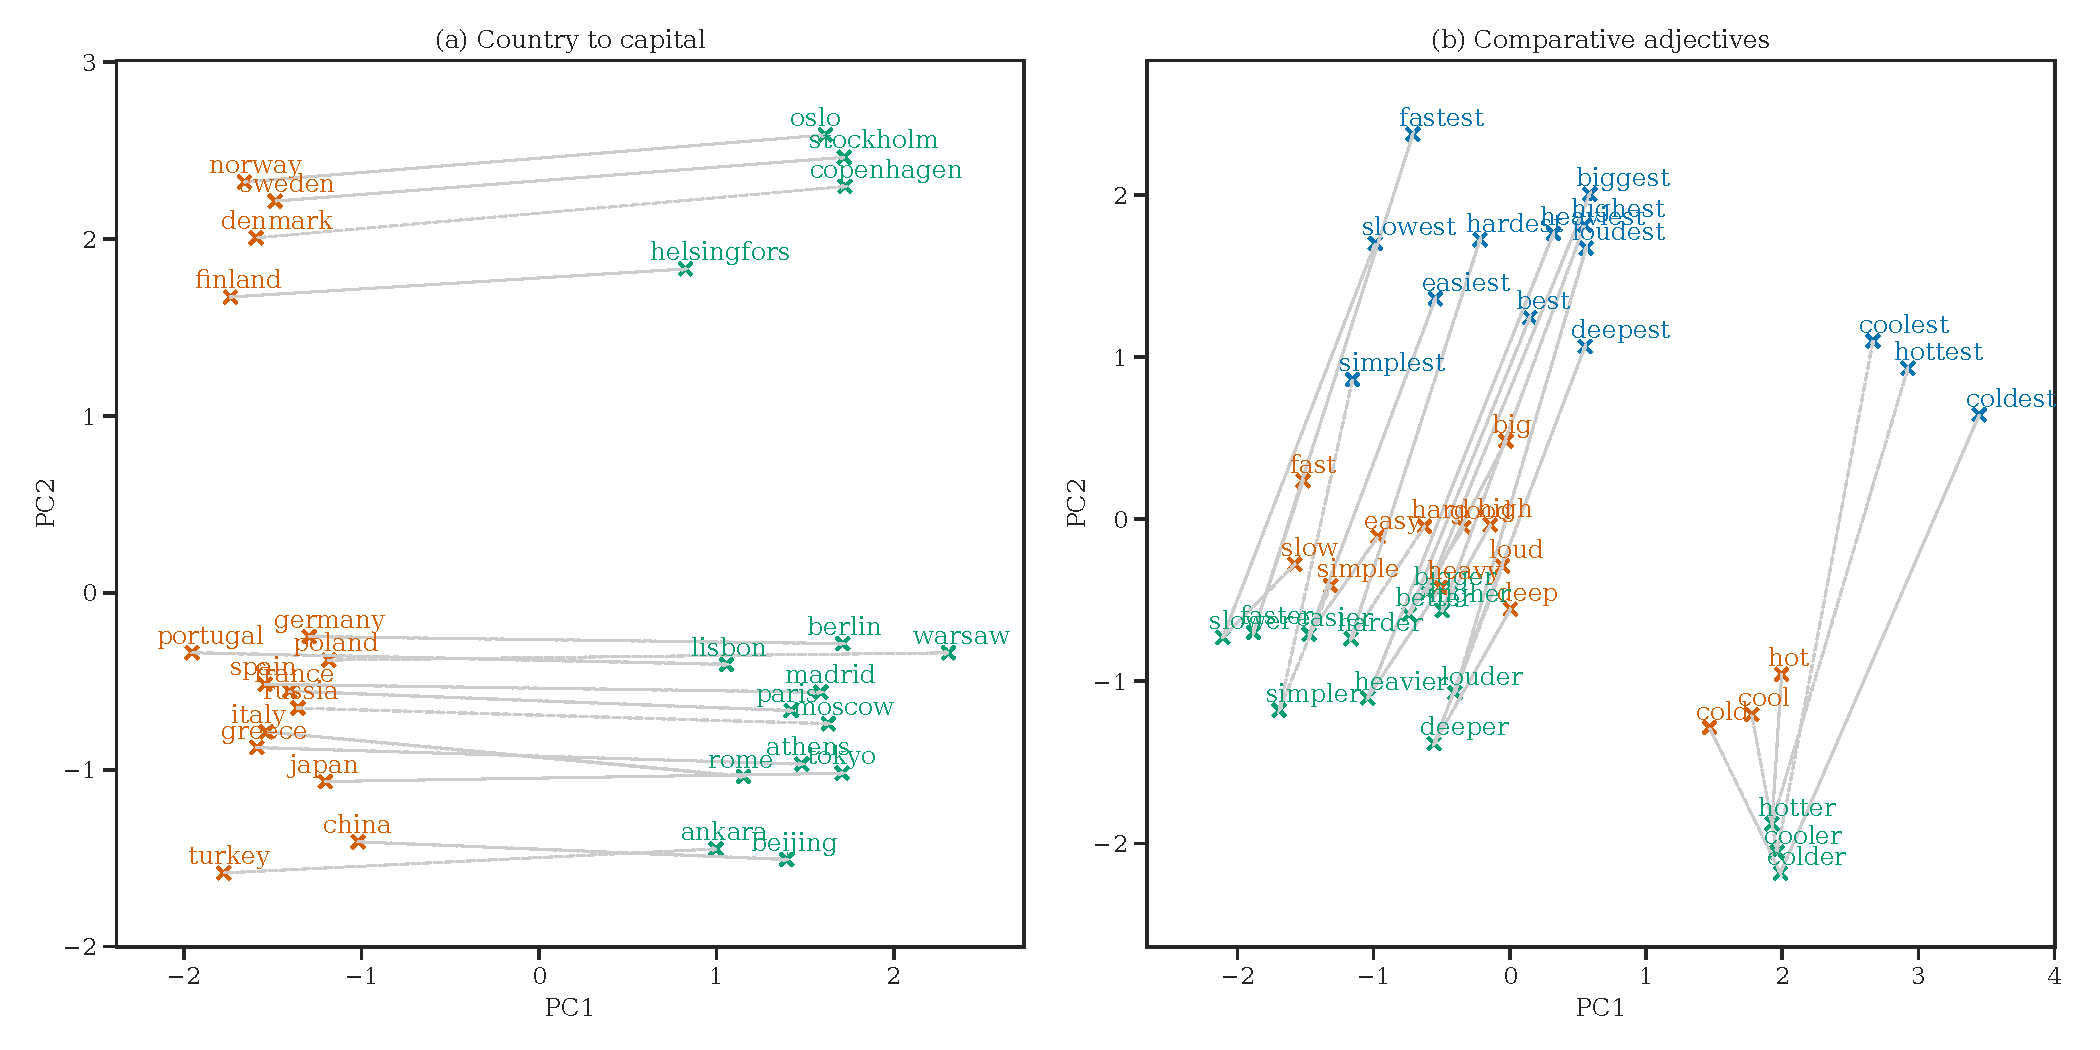
\includegraphics[width=\textwidth]{thesis/figures/word-to-word-relationships-pca-2d.pdf}
 \caption{2-dimensional PCA projection of the word embeddings of SGNS-enwiki of some countries and their capital cities (a) and comparative adjectives (b). This figure is inspired by \cite[Figure 2]{mikolov2013b}.}
 \label{fig:sgns-enwiki-word-to-word-relations-pca-2d}
\end{figure}

Due to the apparent clustering occurring in both plots from \cref{fig:sgns-enwiki-word-to-word-relations-pca-2d}, we will investigate the notion of clustering further. To deepen our understanding of the underlying structure of the SGNS-model, we will in the next section perform cluster analysis of its word embeddings. In particular, we will use multiple clustering algorithms and internal cluster validation methods to find the most suitable clustering algorithm and the number of clusters.
\section{Word clustering}
\label{sec:analysis-of-word-embeddings-word-clustering}
In this section, we will apply cluster analysis on the word embeddings of the SGNS-enwiki, in order to search for deeper structures within the data. In particular, we will compare clustering algorithms on the word embeddings of the SGNS-enwiki in \cref{sec:comparing-clustering-algorithms}, and following, we will look at clustering of distinct groups of words in \cref{sec:clustering-word-groups}.

\subsection{Comparing clustering algorithms}
\label{sec:comparing-clustering-algorithms}
In this subsection, we compare clustering algorithms on the word embeddings of the SGNS-enwiki. Due to the large number of words in the vocabulary of the SGNS-enwiki (roughly 4.4 million, see \cref{sec:word2vec-hyperparameter-choices} for more details), we restrict the analysis to the 10000 most common (i.e most frequently occurring) words. This way, we speed up the computation by reducing the computational requirement, but should still get a reasonable result, as the most common words yield good quality vector representations (more data $\rightarrow$ better vectors).

To perform the cluster analysis, we use all clustering algorithm from \cref{sec:clustering-algorithms}, except for Spectral clustering (\cref{sec:spectral-clustering}), as it was too computationally expensive for it to run. In particular, we used the following algorithms: k-means clustering (\cref{sec:k-means-clustering}), mini-batch k-means clustering (\cref{sec:mini-batch-k-means-clustering}), k-medoids clustering (\cref{sec:k-medoids-clustering}), GMMs (\cref{sec:gmm-clustering}), hierarchical clustering (agglomerative) (\cref{sec:hierarchical-clustering}), HDBSCAN (\cref{sec:hdbscan-clustering}) and ToMaTo (\cref{sec:tomato-clustering}). We used the \path{scikit-learn} \cite{ScikitLearn2011} and \path{hdbscan} \cite{mcinnes2017hdbscan} Python packages to perform clustering. Furthermore, we trained each of the clustering algorithms using a grid-search manner, i.e. by trying all combinations of hyperparameters. \cref{table:hyperparameters-clustering-algorithms} shows the hyperparameters used to train each clustering algorithm. By forming a grid of hyperparameters for each clustering algorithm, we get a rough sense for the best set of hyperparameters. For the initial grid-search, we used the same number of clusters for all the algorithms that allows us to specify the number of clusters. Let \path{n_clusters_range}=2, 3, 4, 5, 10, 50, 100, 150, 200, 300, 400, 500, 750, 1000, 1500, 2000, 3000, 4000, 5000, 6000, 7000, 8000 be the range of cluster numbers used for the initial grid-search. We let \path{n_clusters_range} range from 2 to 8000 clusters, using varying step sizes, to investigate the effect of the number of clusters for each algorithm, where it was applicable. To train the clustering algorithm, we use the standard word embeddings if the algorithm supports cosine similarity (or distance) and normalized word embeddings if the algorithm requires Euclidean distances. After training the clustering algorithms, we validated them using the internal cluster validation methods from \cref{sec:cluster-validation}. In particular, we used the mean Silhouette Coefficient (SC)) (\cref{sec:silhouette-coefficient}), the Davies-Bouldin Index (DBI) (\cref{sec:davies-bouldin-index}) and the Caliński-Harabasz Index (CHI) (\cref{sec:calinski-harabasz-index}). We used the \path{scikit-learn} Python package to perform internal clustering validation.
\begin{table}[H]
    \centering
    \begin{tabular}{@{}lll@{}}
    \toprule
    Clustering algorithm                           & Hyperparameters & Values \\
    \midrule
    \trcolor K-means clustering & \path{n_clusters} & \path{n_clusters_range} \\
    \multirow{2}{*}{Mini-batch k-means clustering} & \path{n_clusters} & \path{n_clusters_range} \\
                                                   & \path{batch_size} & 100 \\
    \trcolor K-medoids clustering & \path{n_clusters} & \path{n_clusters_range} \\
    GMM clustering & \path{n_components} & \path{n_clusters_range} \\
    \trcolor & \path{n_clusters} & \path{n_clusters_range} \\
    \trcolor \multirow{-2}{*}{Agglomerative clustering} & \path{linkage} & \path{single}, \path{average}, \path{complete}, \path{ward} \\
    \multirow{2}{*}{HDBSCAN} & \path{min_cluster_size} & 2, 4, 8, 16, 32, 64 \\
                             & \path{min_samples} & 1, 2, 4, 8, 16, 32, 64\\
    \trcolor                         & \path{density_type} & \path{DTM}, \path{logDTM}, \path{KDE}, \path{logKDE} \\
    \trcolor \multirow{-2}{*}{ToMATo} & \path{k} & 2, 3, \ldots, 10, 20, \ldots, 50, 100, \ldots, 250 \\
    \bottomrule
    \end{tabular}
    \caption{Hyperparameters of clustering algorithms for cluster analysis.}
    \label{table:hyperparameters-clustering-algorithms}
\end{table}

We visualize the result from the initial grid-search in \cref{fig:cluster-analysis-comparison-internal-cluster-validation}. From \cref{fig:cluster-analysis-comparison-internal-cluster-validation}, we see that agglomerative clustering algorithm performs the best (close to k-means clustering) and k-medoids clustering  performs the worst. For this reason, we will now focus on the agglomerative clustering algorithm and search for the best set of hyperparameters, being the linkage criterion and number of clusters.
\begin{figure}[H]
    \centering
    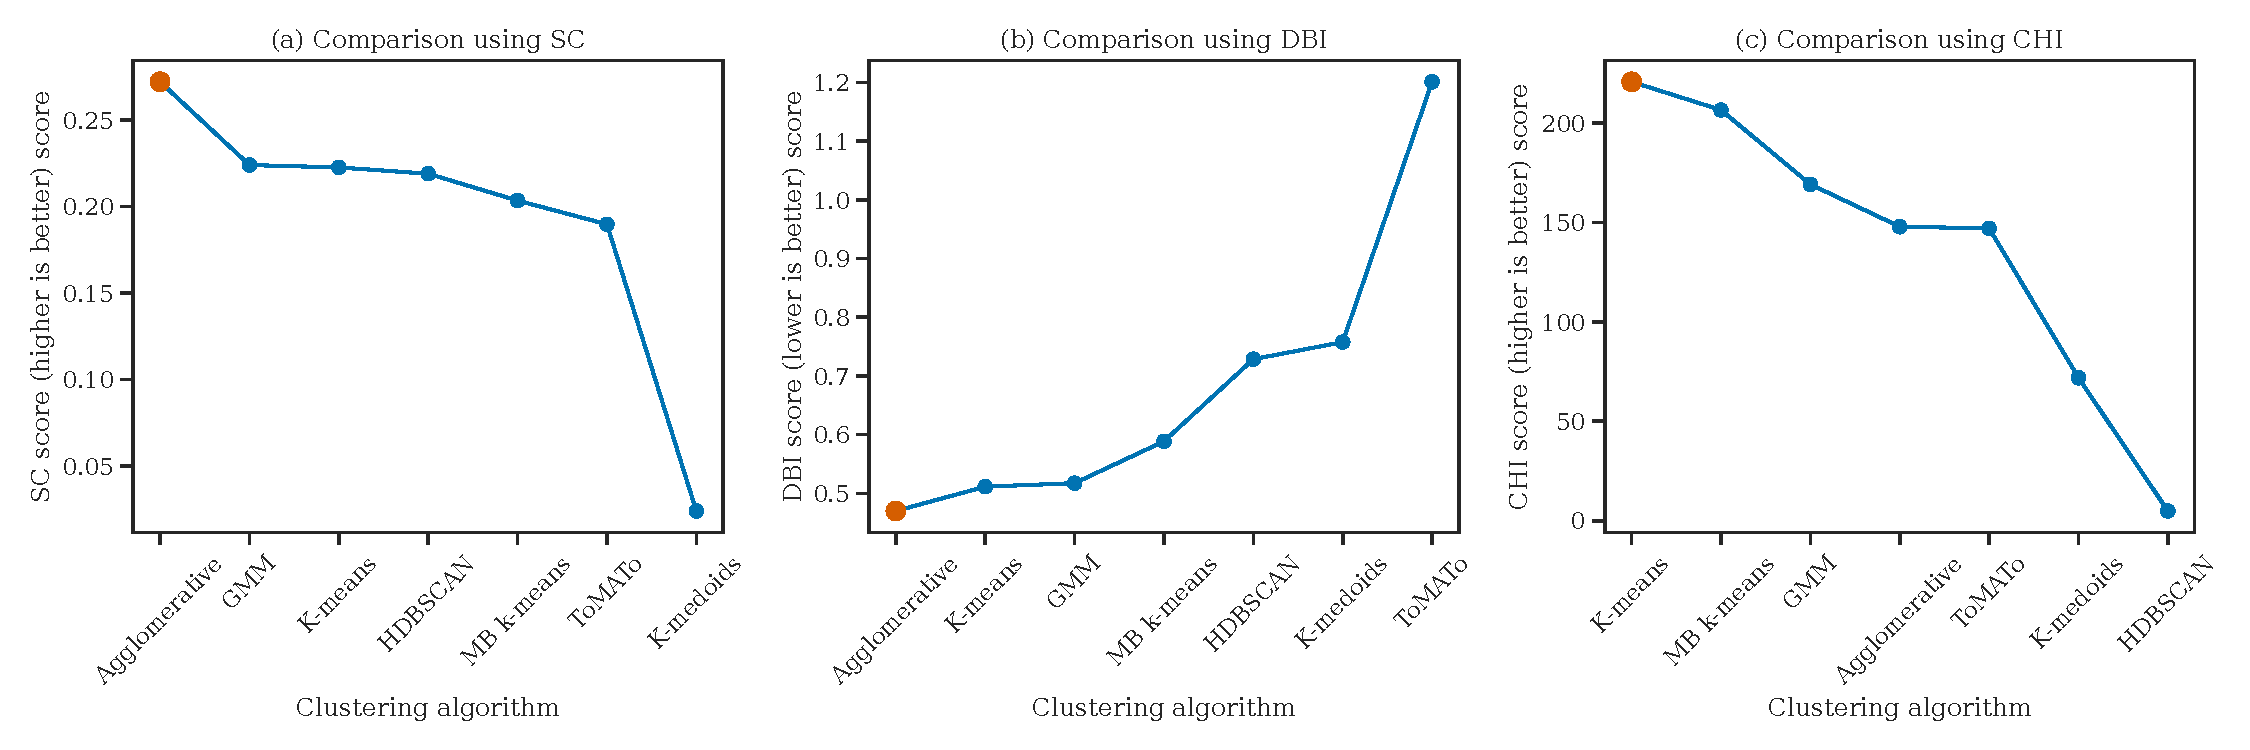
\includegraphics[width=\textwidth]{thesis/figures/cluster-analysis-comparison-internal-cluster-validation.pdf}
    \caption{Comparison of clustering algorithms trained on word embeddings from SGNS-enwiki, ranked by internal cluster validation methods. The red dot in each plot denotes the most optimal value.}
    \label{fig:cluster-analysis-comparison-internal-cluster-validation}
\end{figure}

In order to find the best set of hyperparameters using the agglomerative clustering algorithm, we first visualize its results from the initial grid search in \cref{fig:cluster-analysis-agglomerative-internal-cluster-validation}. From \cref{fig:cluster-analysis-agglomerative-internal-cluster-validation}, first notice that by using the single linkage criterion, we get relatively poor results. The remaining criterions, average, complete and ward, perform more or less the same over all internal clustering validation methods, with the ward criterion being slightly ahead of the rest. By inspecting the best value for the number of clusters for each internal cluster validation method in \cref{fig:cluster-analysis-agglomerative-internal-cluster-validation}, we noticed that the DBI (b) and the CHI (c) gave misleading results, while the SC (a) were more meaningful. In particular, the DBI prefers to have the largest number of clusters, that is, 8000 clusters. We inspected the clusters and observed that 6350 of the words are in its own cluster of size 1. This means that the DBI is not particularly well suited for choosing the number of clusters, as it prefers to have the most clusters. This is also illustrated by looking at the plot in the middle (b) of \cref{fig:cluster-analysis-agglomerative-internal-cluster-validation}. Using the CHI, we observe that it prefers to have the least number of clusters, namely 2. We inspected this result, and noticed that in the first clusters, there were only a single word, while the second cluster had the remaining 9999 words. In other words, this means that the CHI is also not particularly well suited for choosing the number of clusters. Finally, using the SC (a), we observe that the preferred number of clusters lie around 3000 to 6000. We inspected the number of clusters as preferred by average, complete and ward linkage clustering and concluded that they made sense, as there were more variety in the cluster sizes and the number of clusters having the specific each cluster sizes. This indicates that the most preferable number of clusters (using SC) should lie in this range (3000 to 6000), and following, we will narrow down the search for the best number of clusters. For the next experiment, we will not include the single linkage clustering criterion, as it performed poorly.
\begin{figure}[H]
    \centering
    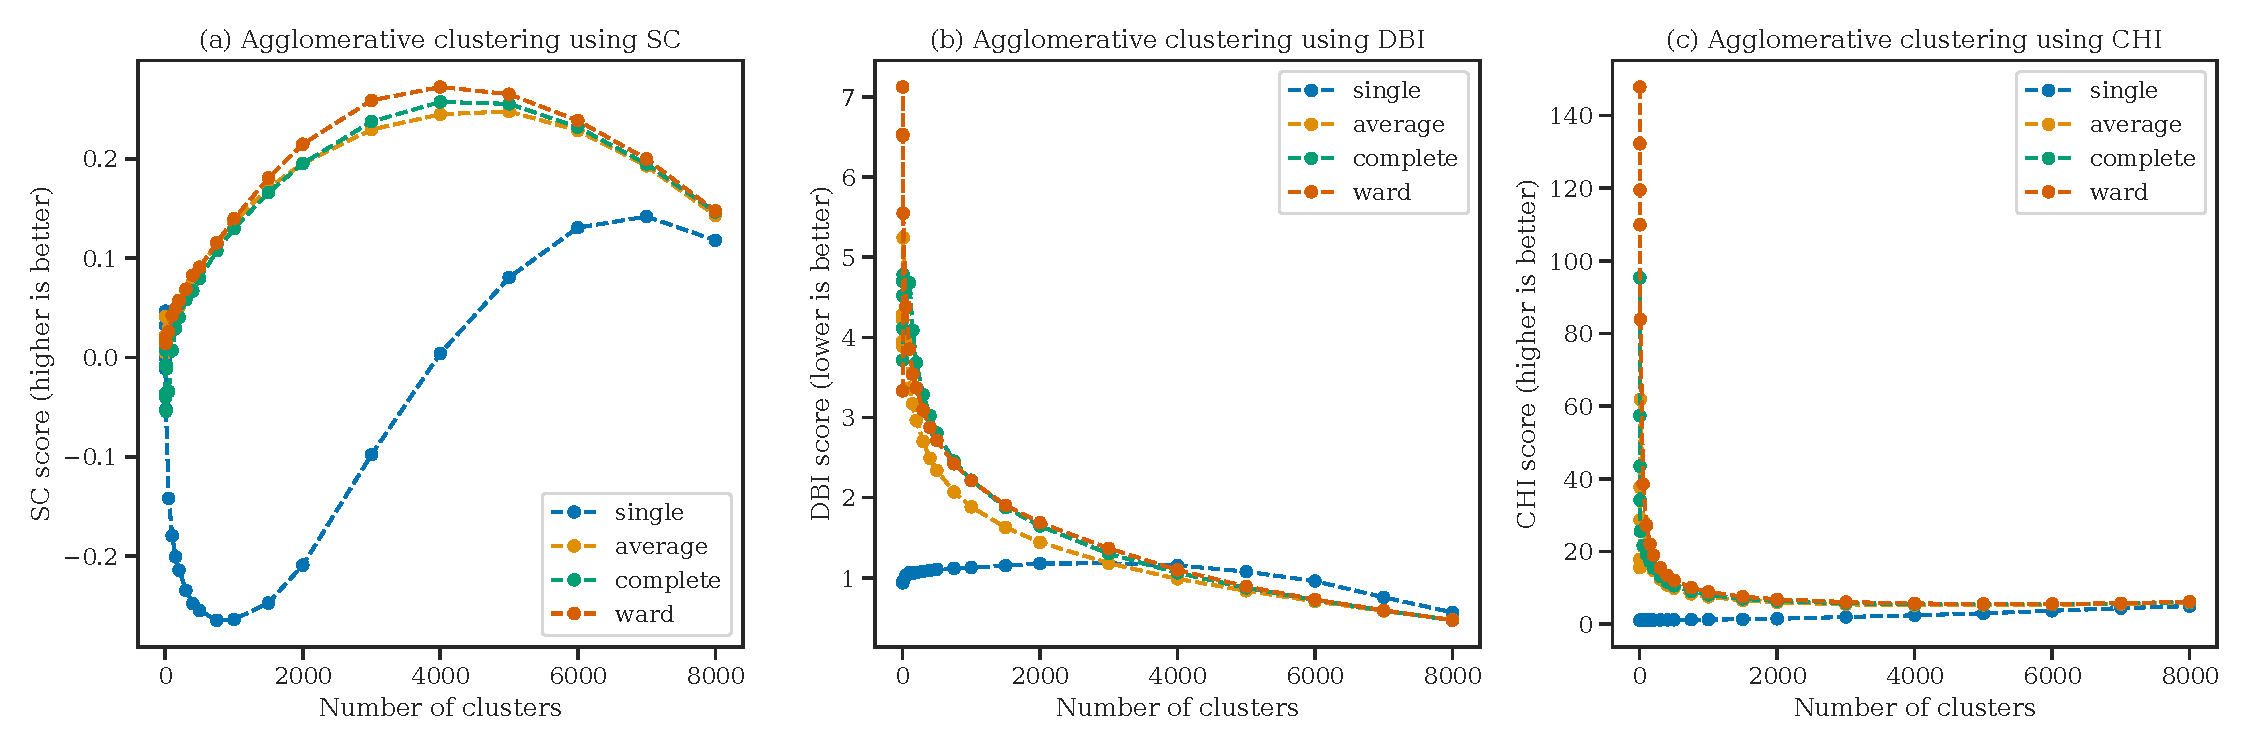
\includegraphics[width=\textwidth]{thesis/figures/cluster-analysis-agglomerative-internal-cluster-validation.pdf}
    \caption{Internal cluster validation results using agglomerative clustering on word embeddings from SGNS-enwiki.}
    \label{fig:cluster-analysis-agglomerative-internal-cluster-validation}
\end{figure}

By narrowing the search to the range 3000 to 6000 clusters, we find the best number of clusters for each criterion, using agglomerative clustering. The narrowed search for number of clusters is shown in \cref{fig:cluster-analysis-agglomerative-internal-cluster-validation-narrow}, and we observe that ward linkage clustering with 4104 clusters result in the best clustering of the 10000 most common words from the SGNS-enwiki model.
\begin{figure}[H]
    \centering
    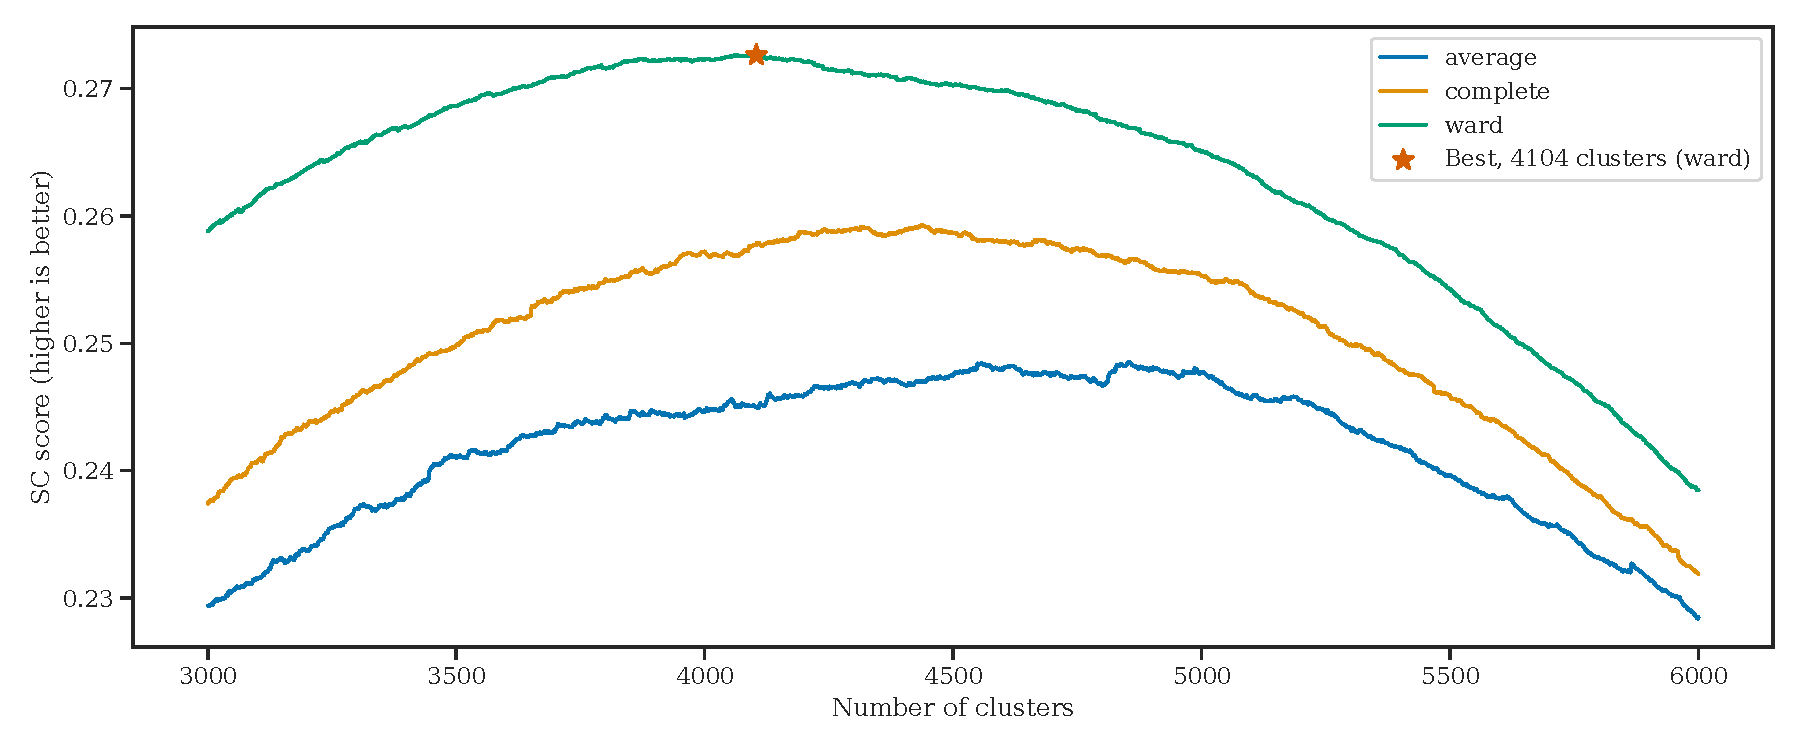
\includegraphics[width=\textwidth]{thesis/figures/cluster-analysis-agglomerative-internal-cluster-validation-narrow.pdf}
    \caption{Number of clusters search using agglomerative clustering and SC, on the range of 3000 to 6000 clusters. Here we see that ward linkage criterion results in the highest SC score.}
    \label{fig:cluster-analysis-agglomerative-internal-cluster-validation-narrow}
\end{figure}

To further gain knowledge of what the best clustering using agglomerative clustering on the word embeddings from SGNS-enwiki, we investigate the words falling into the 4104 clusters, with agglomerative clustering and ward criterion. In particular, we look at the 10 largest and smallest clusters. For the smallest clusters, we look at clusters of size 2 or more, to ensure we do not have clusters consisting of single words. In the top 10 largest clusters, we mostly see names such as "Smith", "Wilson" or "Taylor" being clustered into the same cluster. We also see words representing numbers being clustered together, e.g. "forty-five", "thirty-two" or "fifty-one", and family related words being clustered together, e.g. "father", "son" and "brother". The top 10 smallest clusters mostly consist of words that are strongly related to one another, such as "Adam" and "Noah", "card" and "cards", or "interior" and "exterior". We visualize some of the largest and smallest clusters in \cref{fig:cluster-analysis-agglomerative-2d-umap-top-clusters}, using a 2-dimensional UMAP (\cref{sec:umap}) embedding. To create the UMAP embedding, we used the \path{umap-learn} Python package \cite{mcinnes2018umap-software}, and let \path{n_neighbors=15} and \path{min_dist=0.1}. From \cref{fig:cluster-analysis-agglomerative-2d-umap-top-clusters}, we see that the clusters are widely spread all over the UMAP embedding. In addition to this, the UMAP embedding suggests that there are more clusters throughout the word embeddings, which the clustering algorithms simply were unable to pick up (when evaluated using internal cluster validation methods). We will investigate this further, and in the next subsection, we will look at clustering of distinct word groups. In particular, we will see if bigger sets of words cluster together in the UMAP embedding, suggesting that the word embeddings contains deeper structure.
\begin{figure}
    \centering
    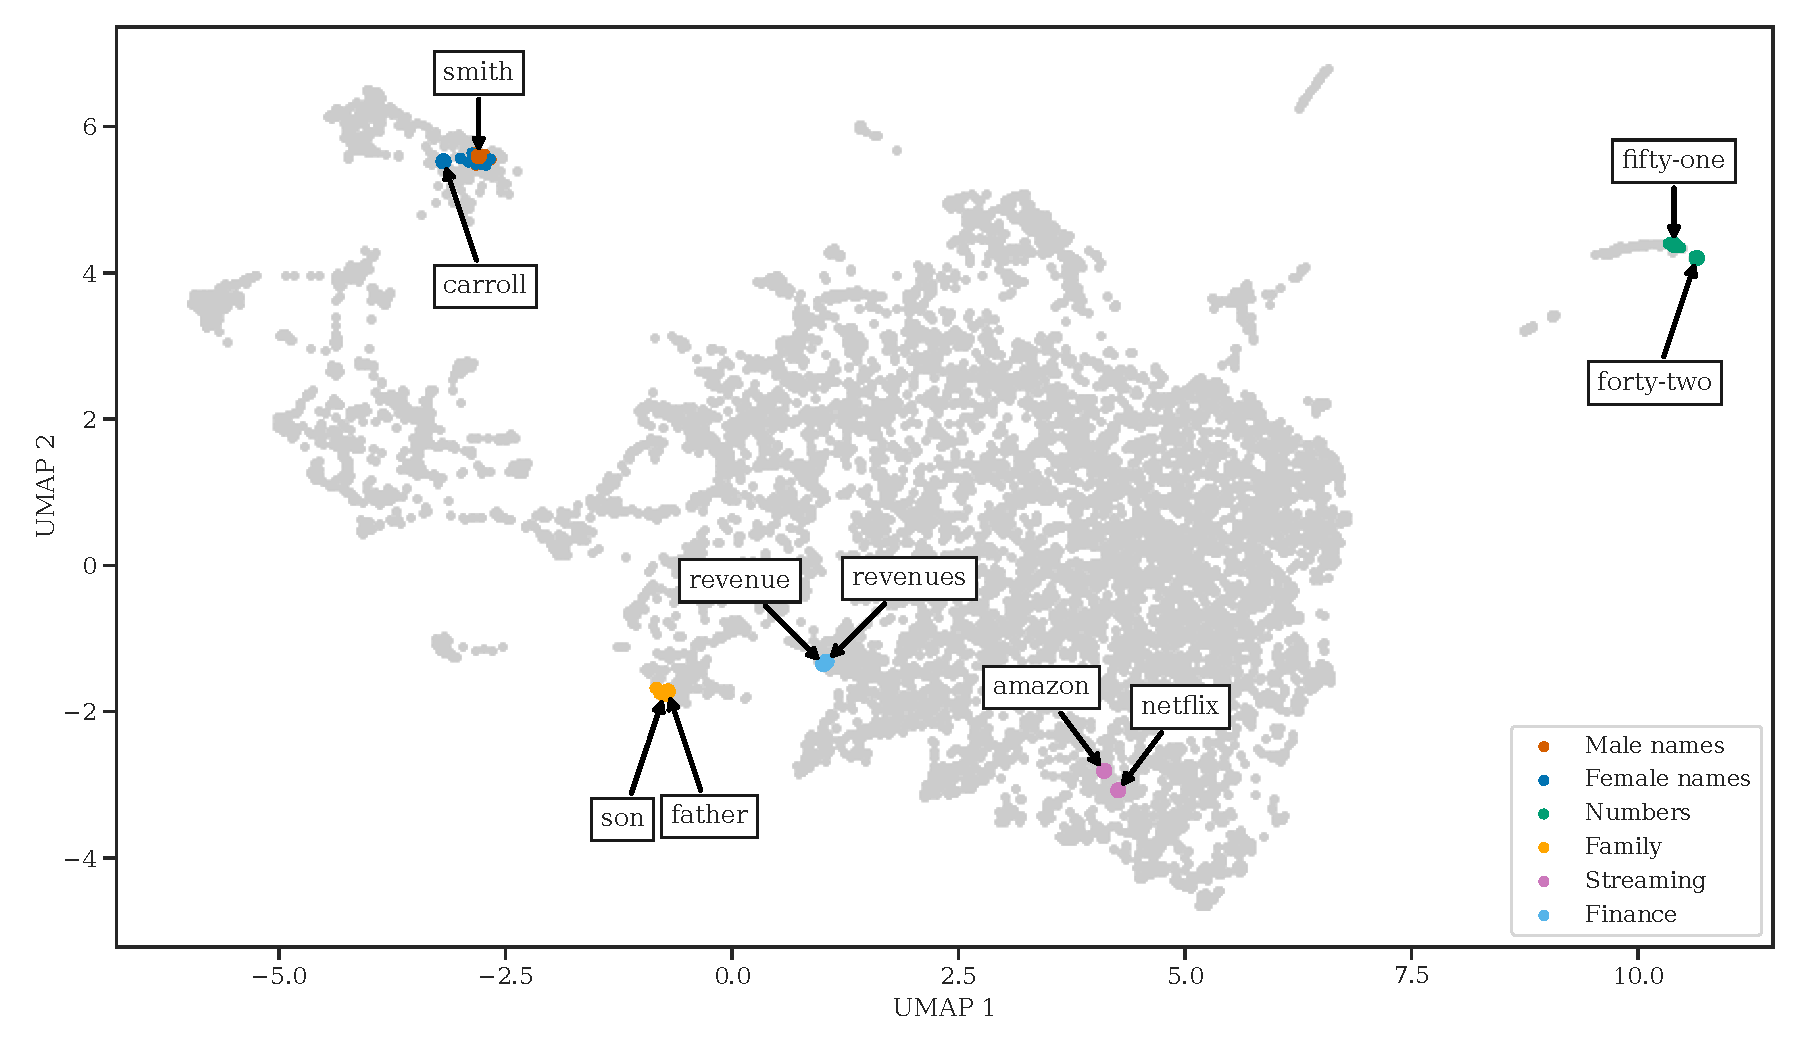
\includegraphics[width=\textwidth]{thesis/figures/cluster-analysis-agglomerative-2d-umap-top-clusters.pdf}
    \caption{2-dimensional UMAP embedding of the 10000 most common words from the SGNS-enwiki model, with some of the largest/smallest clusters outlined.}
    \label{fig:cluster-analysis-agglomerative-2d-umap-top-clusters}
\end{figure}

\subsection{Clustering word groups}
\label{sec:clustering-word-groups}
In this subsection, we will investigate the effect of clustering in the 2-dimensional UMAP embedding of the 10000 most common words of the SGNS-enwiki model, using distinct groups of words. In particular, we will cluster words related to countries/capitals, numbers, names (fore- and surnames) and food. Prior to performing the clustering, we first prepare the data to be used for the analysis. The countries/capitals data was retrieved from \cite{GeoNames}, where we used their API in order to fetch countries and its capital, resulting in 217 pairs of countries and capitals that were in the SGNS-enwiki vocabulary. The number data was generated by converting numbers to its string representation. We converted the numbers from zero to one trillion, resulting in 105 number related words. The forenames data was retrieved from \cite{SSABabyNames}, where we used the top 1000 baby names from 2019. The surnames data was retrieved from \cite{CensusSurnames}, and we used the top 1000 surnames from 2010. Finally, the food data was retrieved from \cite{FoodIngredientList}, where we used the 250 most common ingredient words. We visualize the largest clusters of word groups falling into the 10000 most common words from the SGNS-enwiki word embeddings, embedded into a 2-dimensional UMAP embeddings in \cref{fig:word-cluster-all-groups}. From \cref{fig:word-cluster-all-groups}, we observe that there are two well separated clusters forming in the UMAP embedding, namely the names and numbers word groups. The countries and food groups are more spread out in the embedding.
\begin{figure}[H]
    \centering
    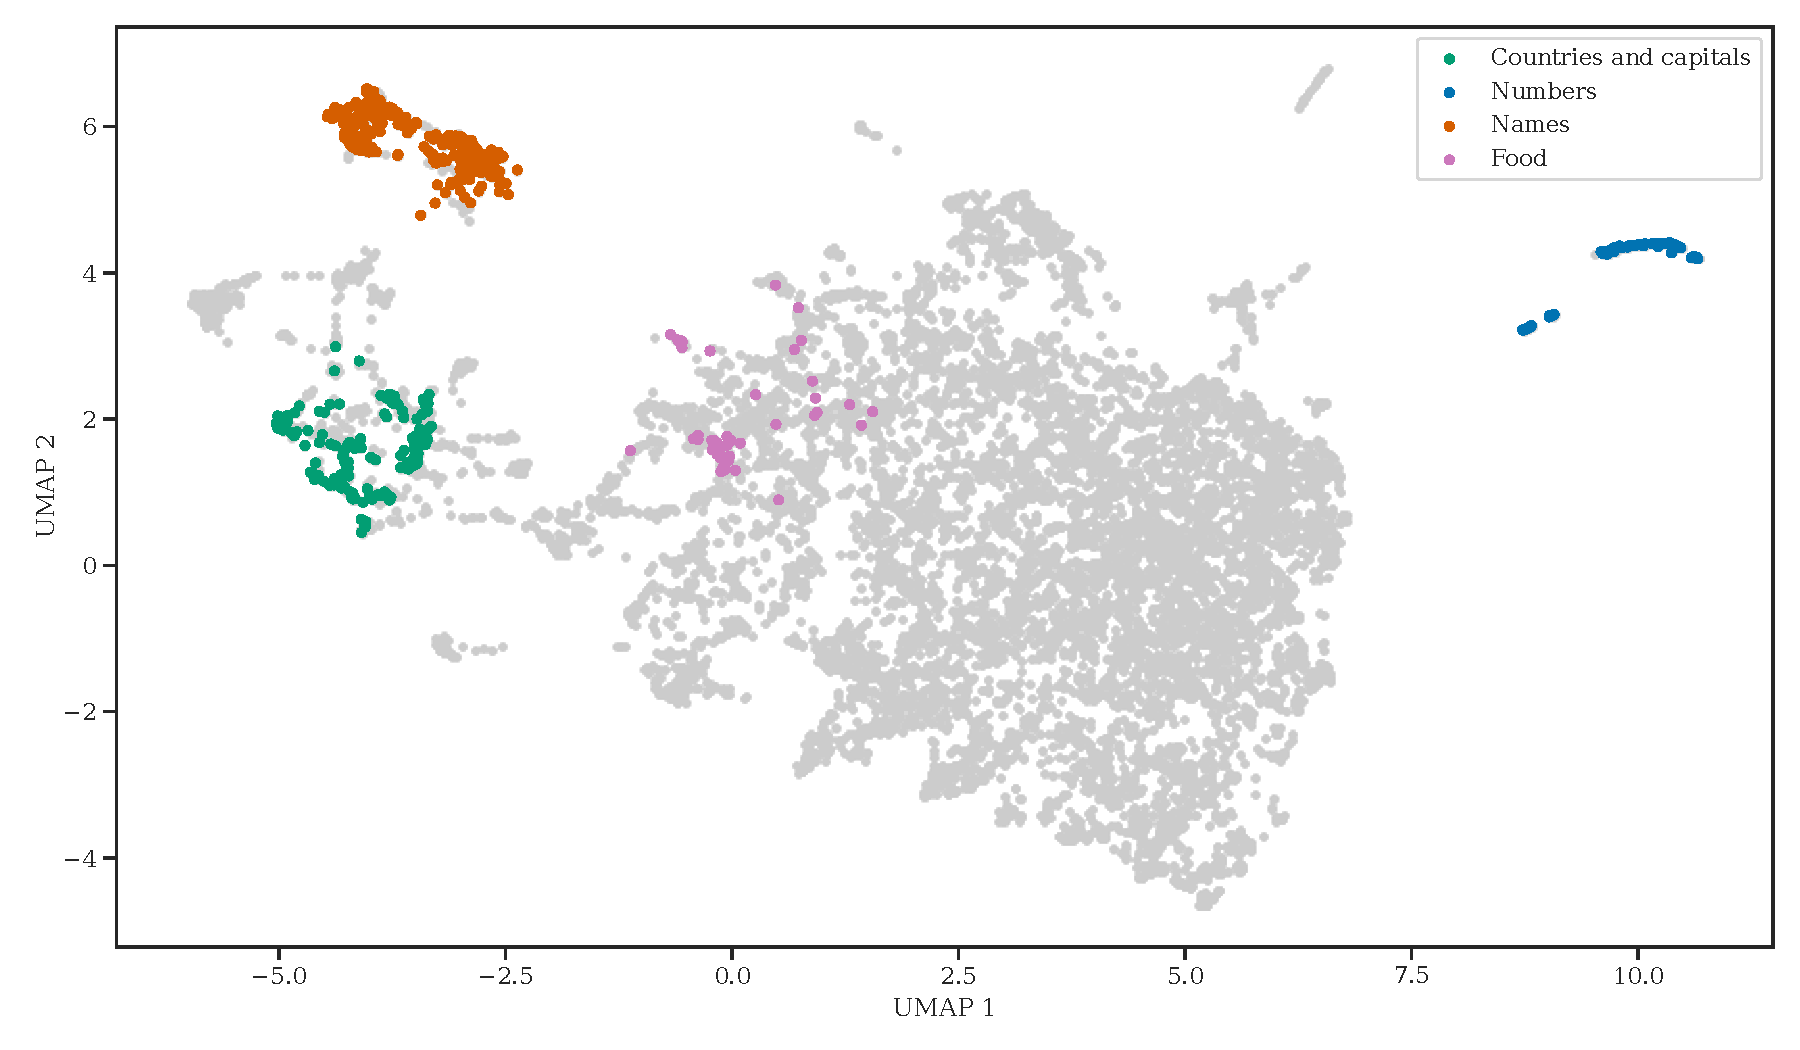
\includegraphics[width=\textwidth]{thesis/figures/word-cluster-all-groups.pdf}
    \caption{2-dimensional UMAP embedding of the 10000 most common words from the SGNS-enwiki model, with word groups outlined.}
    \label{fig:word-cluster-all-groups}
\end{figure}

Note that, in \cref{fig:word-cluster-all-groups}, we have outlined the largest clusters of the word groups, and discarded words falling out of the largest clusters. By including words that are outside the largest clusters, we saw that, in particular, the names word group is spread throughout the word embedding, as the data we used contained fore- and surnames of common words, such as "joy", "page" or "good". We illustrate this behaviour in \cref{fig:word-cluster-all-groups-emphasis-plots}, where we outline the four different word groups. From \cref{fig:word-cluster-all-groups-emphasis-plots}, we see that the country and capital words (a) are mostly clustered to the middle left, with some capitals falling out of the bigger cluster. The "Stanley" and "Hamilton" capital cities are also used as names, indicated by the names (c) plot. For the numbers, we observe that most number related words are clustered to the right, clearly separated from the rest of the words. However, we also observe that words such as "million", "billion" and "trillion" are clustered together outside the numbers cluster to the right. By inspection, we observed that the "million", "billion" and "trillion" words were in fact close to other financial words, such as "banks", "wealth" or "economics". For the names (c), we see that the fore- and surnames are clustered to the top right, but also spread throughout the UMAP embedding. We also observe a small cluster of woman names forming, containing the names "Diana" and "Isabella". Lastly, we see that food related words (d) are slightly clustered around the words "egg" and "cheese", but also slightly spread around the UMAP embedding. An interesting observation is the word "apple", which is both a fruit and a technology company. In this case, the word apple refers to the company Apple Inc., as we also saw earlier in \cref{table:word2vec-nearest-neighbours-words}.
\begin{figure}[H]
    \centering
    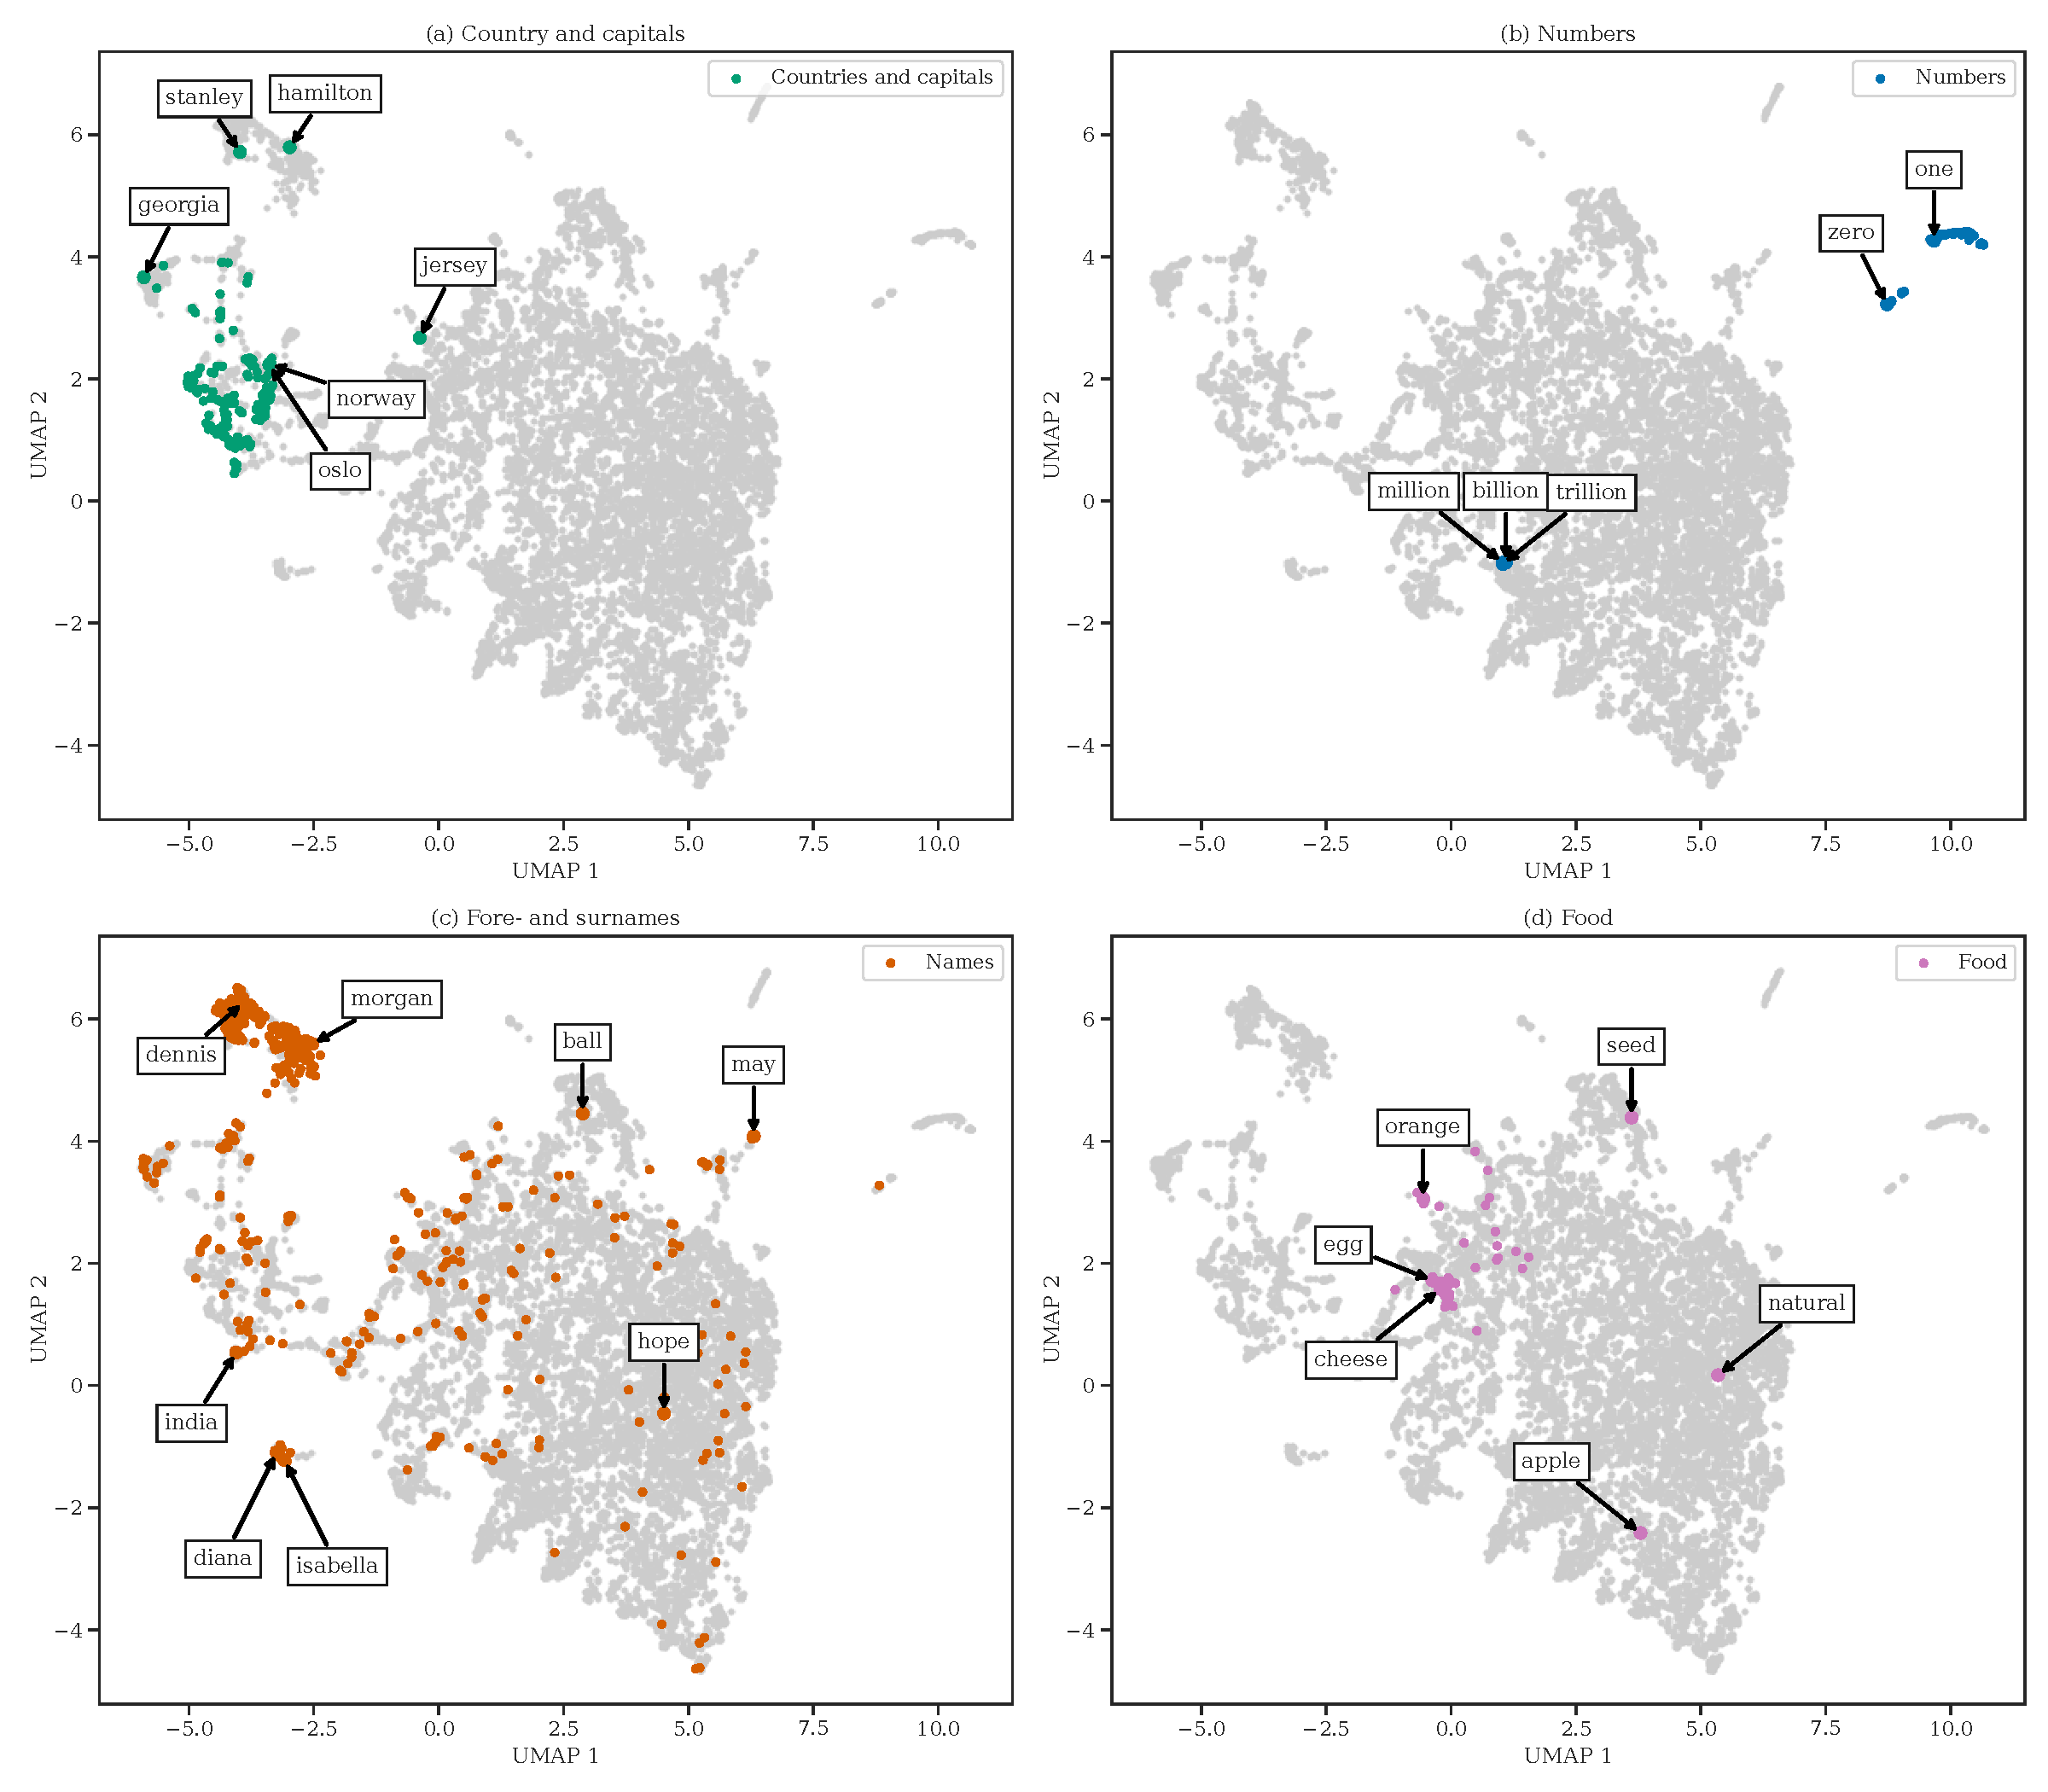
\includegraphics[width=\textwidth]{thesis/figures/word-cluster-all-groups-emphasis-plots.pdf}
    \caption{2-dimensional UMAP embeddings of the 10000 most common words from the SGNS-enwiki model. Here we see four plots, where in each plot we have outlined the four different word groups.}
    \label{fig:word-cluster-all-groups-emphasis-plots}
\end{figure}

We will now further analyze two of the word groups to further develop our understanding of the word embeddings. In particular, we will perform cluster analysis of the word embeddings of countries/capitals and numbers, where we will use clustering algorithms to cluster the words. We will use the same clustering algorithms specified in \cref{sec:comparing-clustering-algorithms}, in addition to Spectral clustering. In order to visualize the results, we will use dimensionality reduction algorithms to create 2-dimensional embeddings. We will also use latitude/longitude coordinates of countries in order to visualize the clustering results using countries/capitals word embeddings.

We analyze the countries and capital word groups separately, as we choose to either identify a country by its name or its capital. Starting with the country word group, we perform cluster analysis. The result of the cluster analysis is summarized in \cref{fig:cluster-analysis-country-word-group-internal-cluster-validation}. There we see a similar result to the result shown in \cref{fig:cluster-analysis-comparison-internal-cluster-validation}, namely that agglomerative clustering is the preferred choice of clustering algorithm.
\begin{figure}[H]
    \centering
    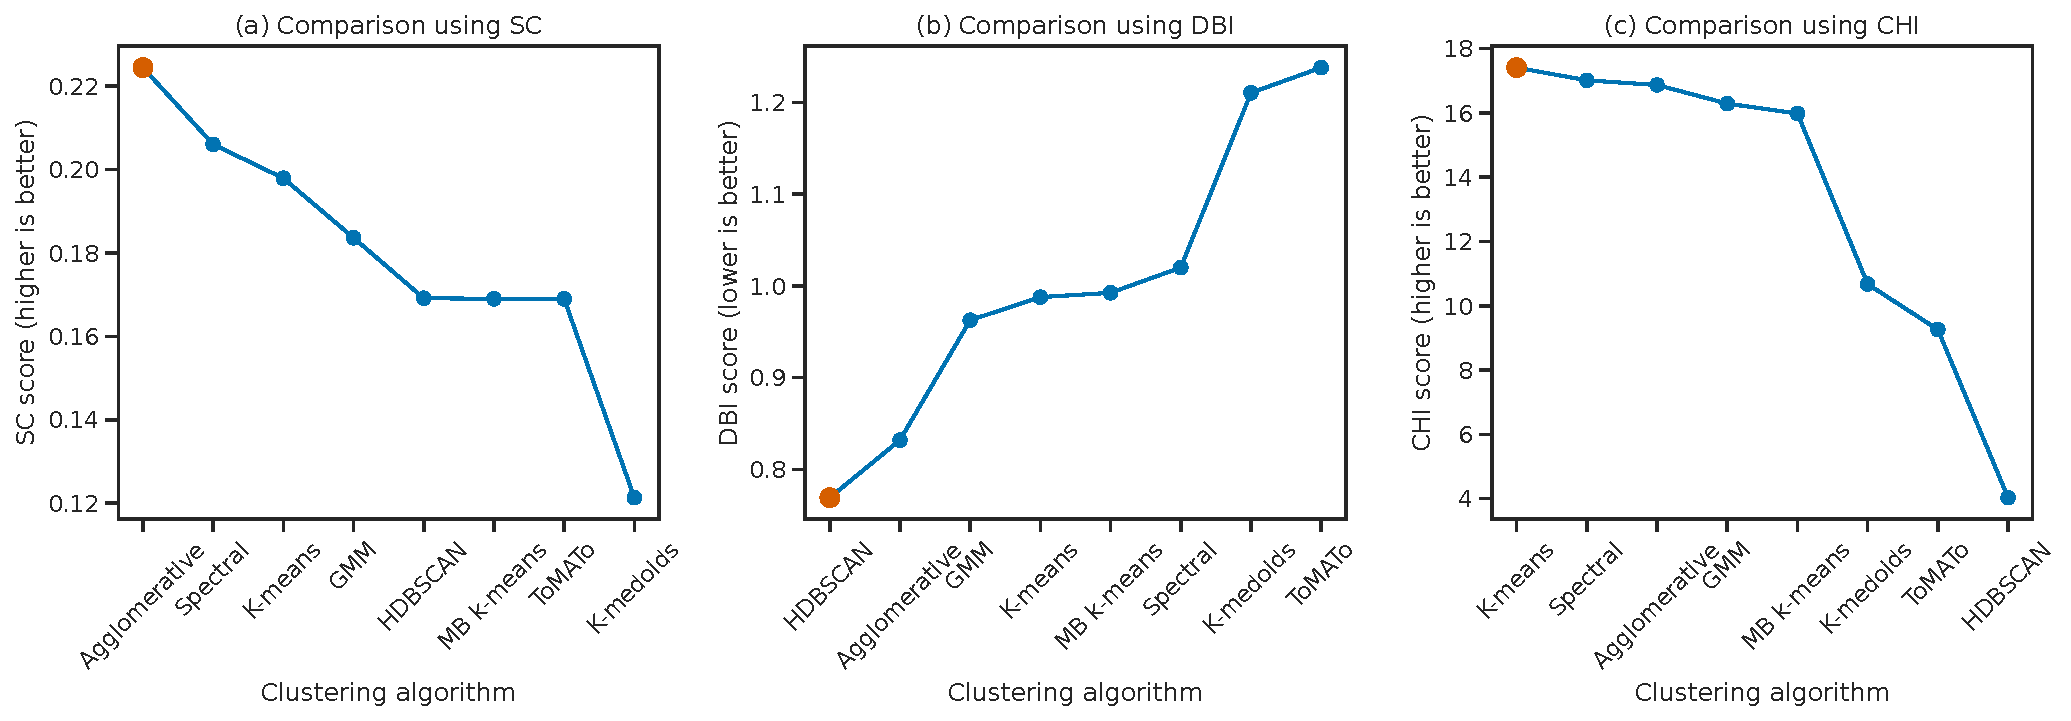
\includegraphics[width=\textwidth]{thesis/figures/cluster-analysis-country-word-group-internal-cluster-validation.pdf}
    \caption{Comparison of clustering algorithms trained on country word embeddings from SGNS-enwiki, ranked by internal cluster validation methods. The red dot in each plot denotes the most optimal value.}
    \label{fig:cluster-analysis-country-word-group-internal-cluster-validation}
\end{figure}

Following, we inspected the scores from the DBI and CHI methods and observed a similar pattern to the analysis from \cref{sec:comparing-clustering-algorithms}, namely that DBI prefers every word to be in its own cluster and CHI prefers to have the smallest number of clusters (i.e. 2). For this reason, we mainly focus on the results using SC. Using agglomerative clustering, we visualize its result in \cref{fig:cluster-analysis-agglomerative-country-word-group-internal-cluster-validation}. From \cref{fig:cluster-analysis-agglomerative-country-word-group-internal-cluster-validation}, we see similar results to \cref{fig:cluster-analysis-agglomerative-internal-cluster-validation}, namely that ward criterion gives the best clustering when using agglomerative clustering.
\begin{figure}[H]
    \centering
    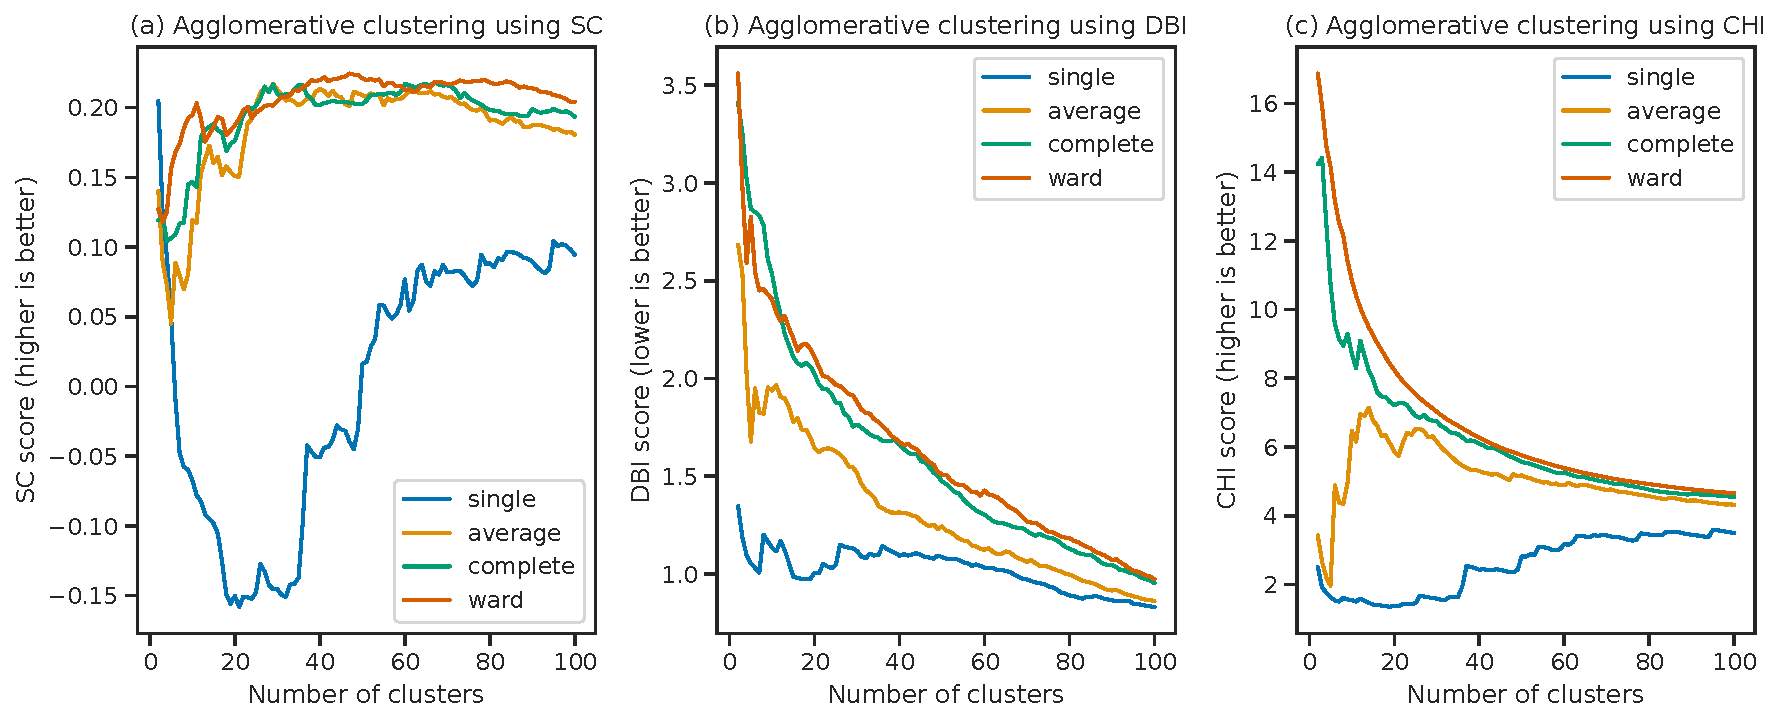
\includegraphics[width=\textwidth]{thesis/figures/cluster-analysis-agglomerative-country-word-group-internal-cluster-validation.pdf}
    \caption{Internal cluster validation results using agglomerative clustering on country word embeddings from SGNS-enwiki.}
    \label{fig:cluster-analysis-agglomerative-country-word-group-internal-cluster-validation}
\end{figure}

The best clustering using SC with agglomerative clustering and ward criterion resulted in 47 clusters. We visualize this result using latitude/longitude coordinates of each country by emphasizing the five largest clusters in \cref{fig:cluster-analysis-agglomerative-country-word-group-top-clusters}. From \cref{fig:cluster-analysis-agglomerative-country-word-group-top-clusters}, we see that the top 5 largest clusters are clustered together in the same continent.
\begin{figure}[H]
    \centering
    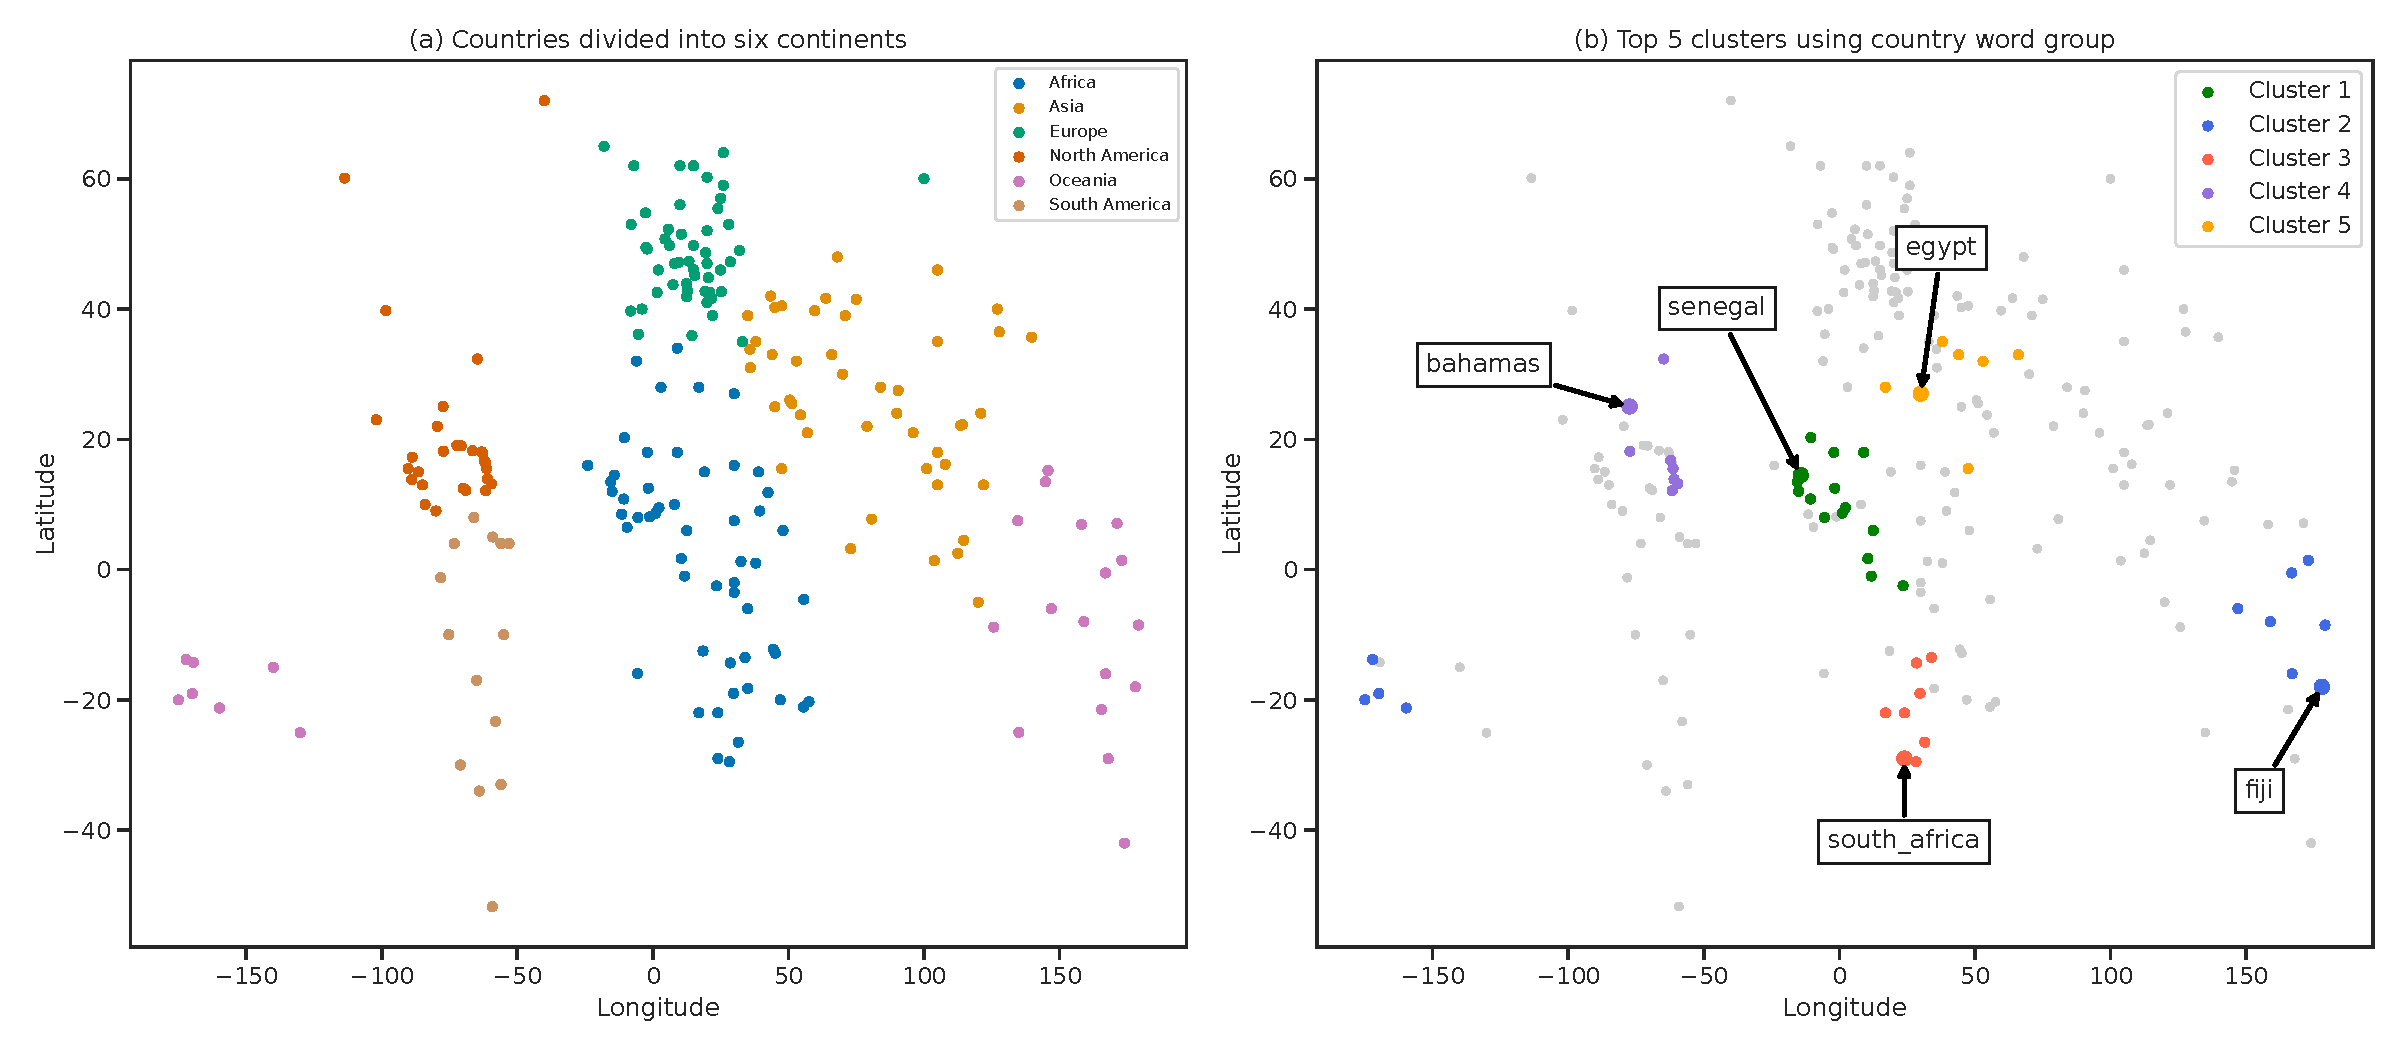
\includegraphics[width=\textwidth]{thesis/figures/cluster-analysis-agglomerative-country-word-group-top-clusters.pdf}
    \caption{Comparison of countries clustered into their respective continents (a) versus top 5 largest clusters from clustering of country word embeddings from SGNS-enwiki using agglomerative clustering and ward criterion. Here we can see that the top 5 largest clusters using agglomerative clustering correlate well with the continent of the respective countries.}
    \label{fig:cluster-analysis-agglomerative-country-word-group-top-clusters}
\end{figure}

Furthermore, we repeat the cluster analysis using capital to identify each country. That is, we use the word embeddings of the capital words instead of the previously used country word embeddings. The result of the cluster analysis is summarized in \cref{fig:cluster-analysis-country-capitals-word-group-internal-cluster-validation}. There we see a similar result to the result shown in both \cref{fig:cluster-analysis-comparison-internal-cluster-validation} and \cref{fig:cluster-analysis-country-word-group-internal-cluster-validation}, namely that agglomerative clustering is the preferred choice of clustering algorithm.
\begin{figure}[H]
    \centering
    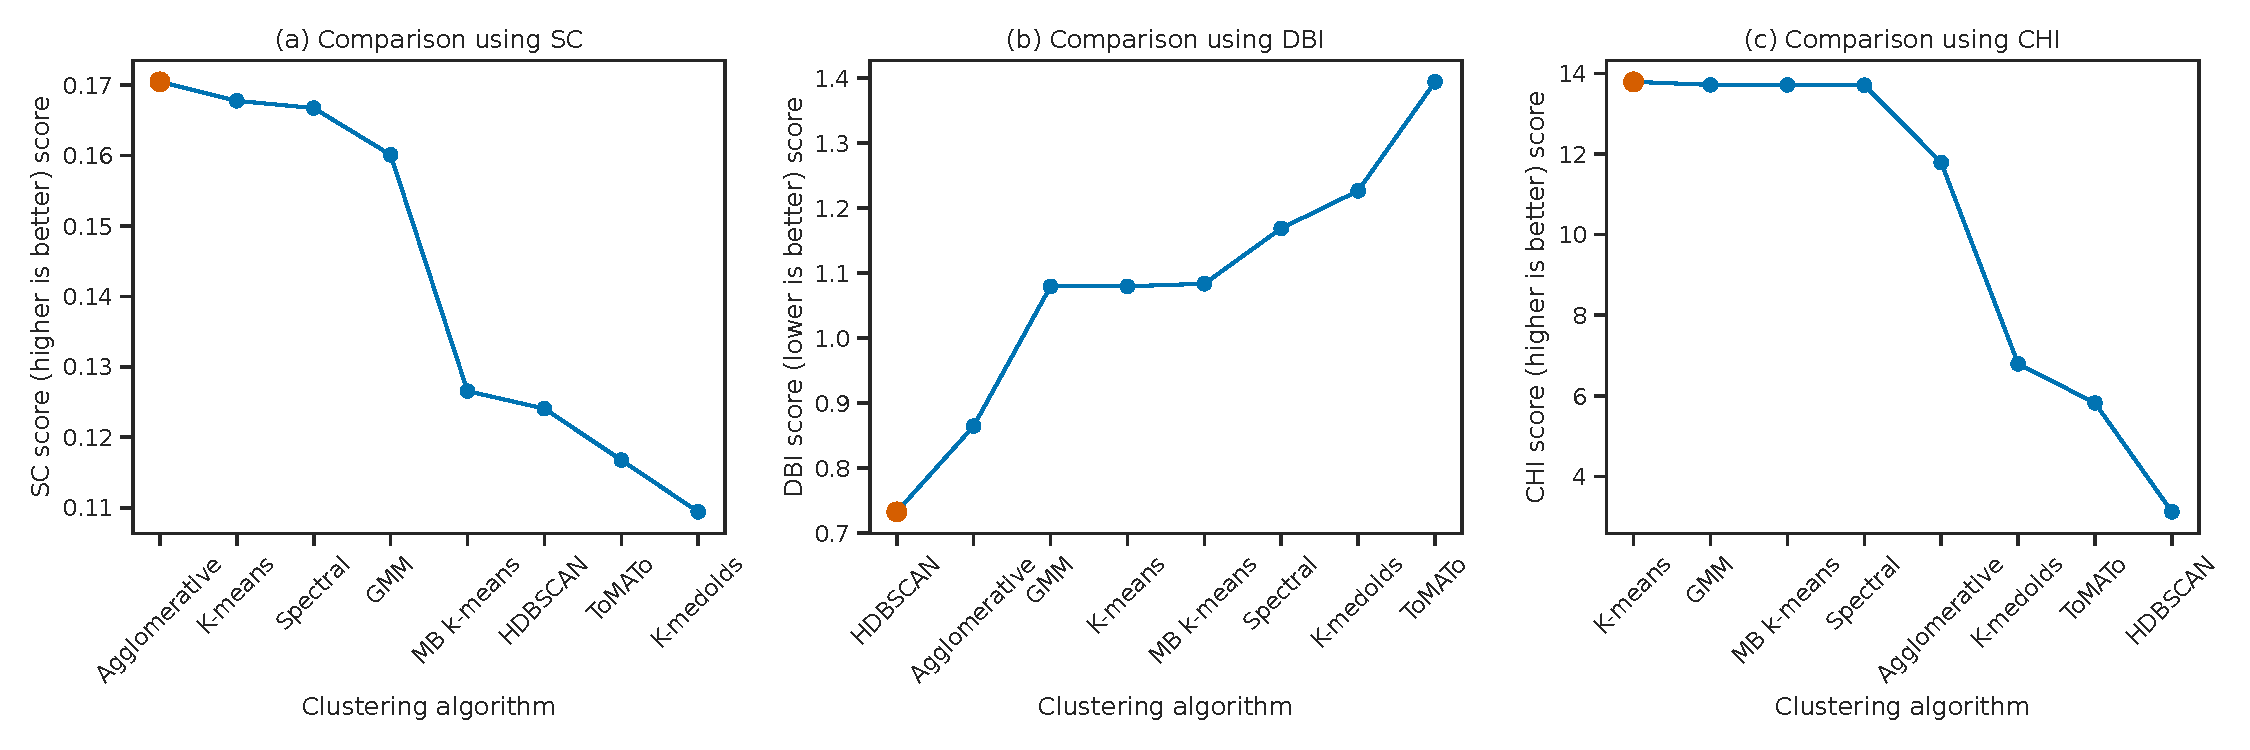
\includegraphics[width=\textwidth]{thesis/figures/cluster-analysis-country-capitals-word-group-internal-cluster-validation.pdf}
    \caption{Comparison of clustering algorithms trained on capital word embeddings from SGNS-enwiki, ranked by internal cluster validation methods. The red dot in each plot denotes the most optimal value.}
    \label{fig:cluster-analysis-country-capitals-word-group-internal-cluster-validation}
\end{figure}

We inspected the scores from the DBI and CHI methods, and similar to the results from \cref{sec:comparing-clustering-algorithms} and the cluster analysis using country word embeddings, we saw that DBI prefers every word to be in its own cluster and CHI prefers to have the smallest number of clusters (i.e. 2). This further strengthens the motivation to use SC over the other methods, and we mainly focus on the results using SC. Using agglomerative clustering, we visualize the results using capital word embeddings in \cref{fig:cluster-analysis-agglomerative-country-capitals-word-group-internal-cluster-validation}. From \cref{fig:cluster-analysis-agglomerative-country-capitals-word-group-internal-cluster-validation}, we see similar results to \cref{fig:cluster-analysis-agglomerative-internal-cluster-validation} and \cref{fig:cluster-analysis-agglomerative-country-word-group-internal-cluster-validation}, namely that ward criterion gives the best clustering when using agglomerative clustering.
\begin{figure}[H]
    \centering
    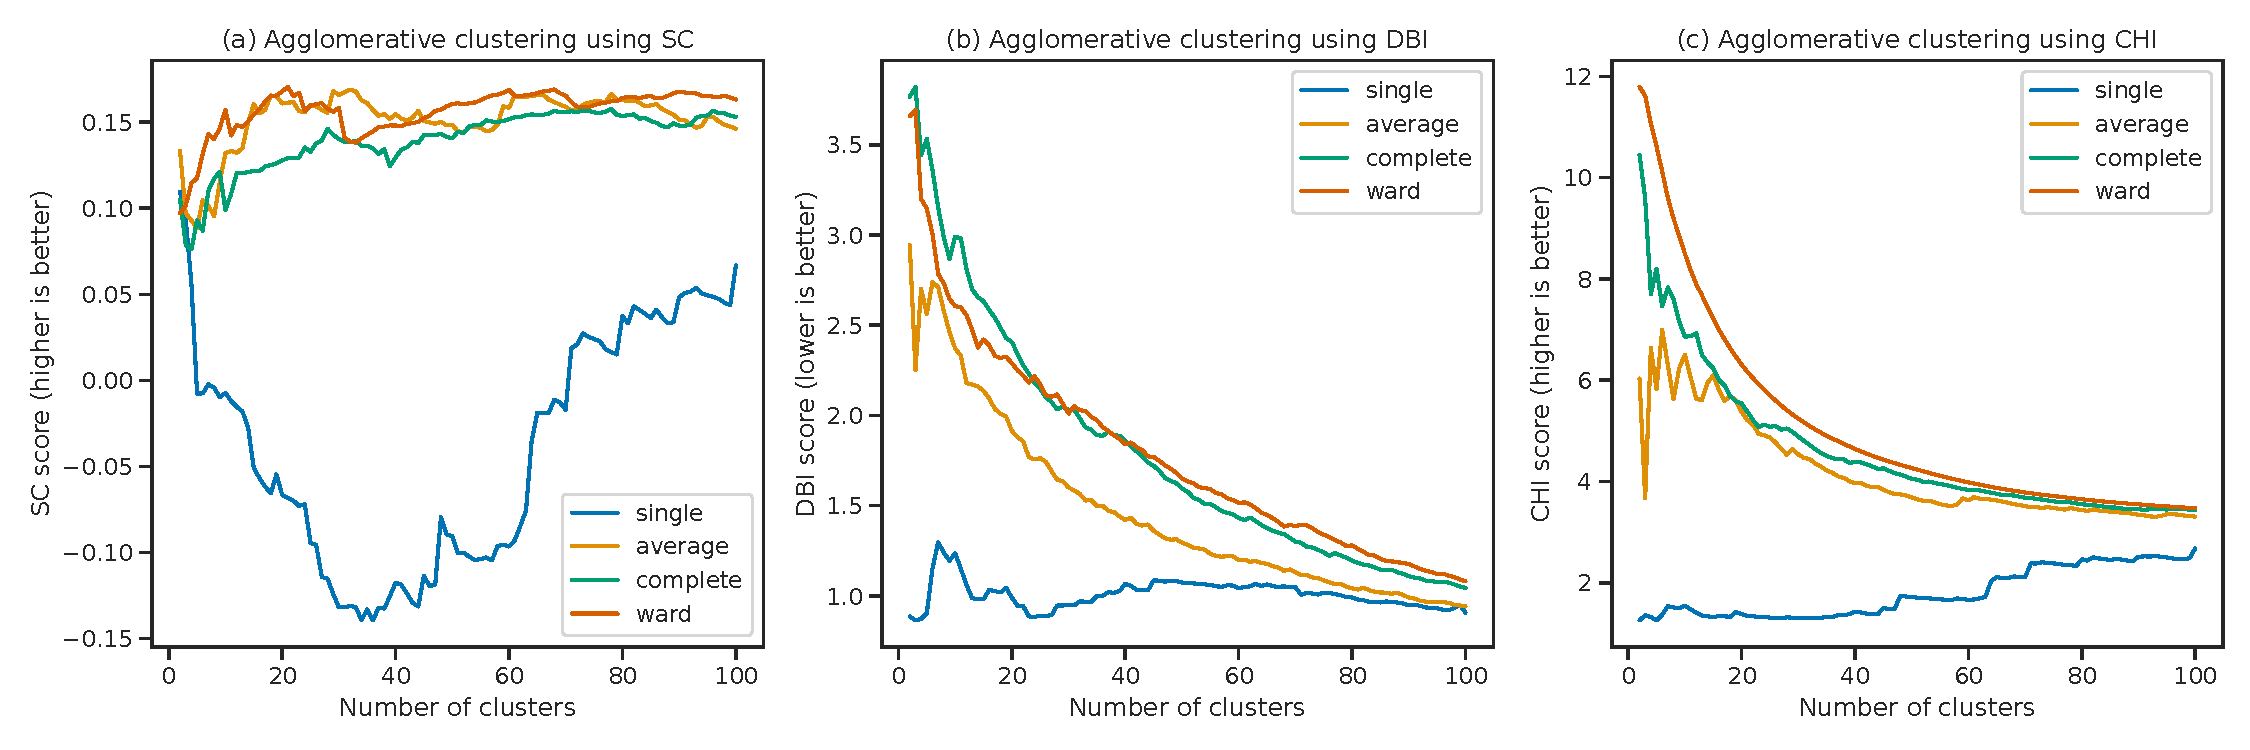
\includegraphics[width=\textwidth]{thesis/figures/cluster-analysis-agglomerative-country-capitals-word-group-internal-cluster-validation.pdf}
    \caption{Internal cluster validation results using agglomerative clustering on capital word embeddings from SGNS-enwiki.}
    \label{fig:cluster-analysis-agglomerative-country-capitals-word-group-internal-cluster-validation}
\end{figure}

The best clustering using SC with agglomerative clustering and ward criterion resulted in 21 clusters. We visualize this result using latitude/longitude coordinates of each country by emphasizing the five largest clusters in \cref{fig:cluster-analysis-agglomerative-country-capitals-word-group-top-clusters}. From \cref{fig:cluster-analysis-agglomerative-country-capitals-word-group-top-clusters}, we see that we get larger clusters than by using country word embeddings in \cref{fig:cluster-analysis-agglomerative-country-word-group-top-clusters}. Furthermore, we observe that in plot (b) the first cluster (green) consists of capitals where the countries are Spanish talking, as outlined by the "Madrid" (Spain), "Mexico City" (Mexico) and "Santiago" (Chile) boxes. The second cluster (blue) in plot (b) also correlates well with the Oceanic continent of plot (a), while the third (red) and forth (purple) clusters of plot (b) seem to capture the African continent very well (Dakar is the capital of Senegal and Pretoria is one of the capitals of South Africa). The last cluster (yellow) consists of capitals from Eastern Europe, as well as some Asian capitals. This concludes the cluster analysis of country and capital word embeddings, and furthermore, we will perform cluster analysis of words related to numbers.
\begin{figure}[H]
    \centering
    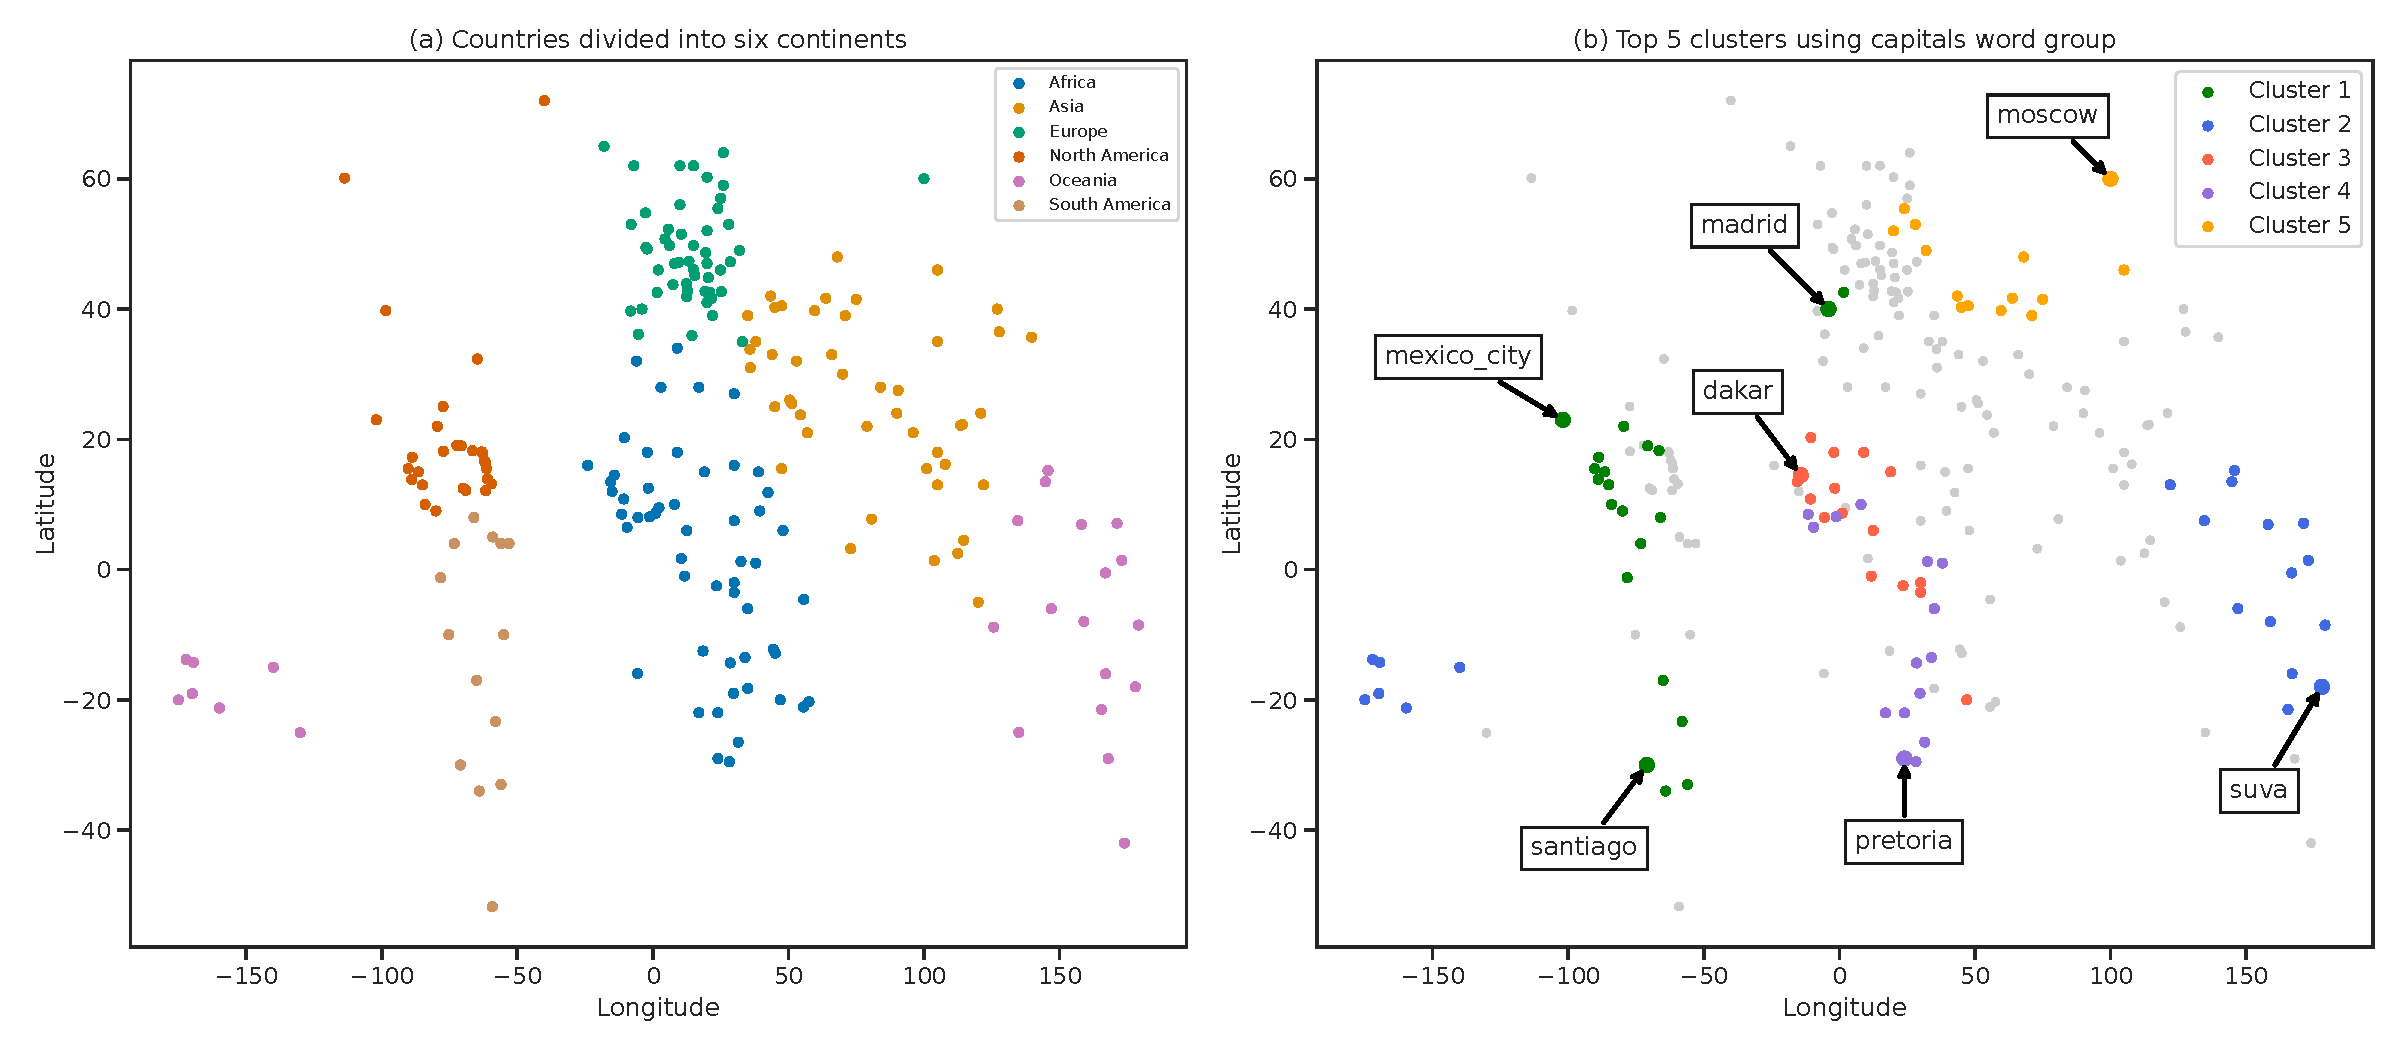
\includegraphics[width=\textwidth]{thesis/figures/cluster-analysis-agglomerative-country-capitals-word-group-top-clusters.pdf}
    \caption{Comparison of countries clustered into their respective continents (a) versus top 5 largest clusters from clustering of capital word embeddings from SGNS-enwiki using agglomerative clustering and ward criterion. From plot (b) we can see that Spanish speaking countries are clustered together in the first cluster (green), while the other clusters are well clustered with regards to the continent of its country.}
    \label{fig:cluster-analysis-agglomerative-country-capitals-word-group-top-clusters}
\end{figure}

We perform cluster analysis of number word embeddings in a similar manner to the cluster analysis of country/capital word embeddings. First, we compare clustering algorithms using internal cluster validation methods, as shown in \cref{fig:cluster-analysis-numbers-word-group-internal-cluster-validation}. From \cref{fig:cluster-analysis-numbers-word-group-internal-cluster-validation}, we see that, overall, the agglomerative clustering algorithm is the best clustering algorithm, when evaluated using internal validation methods.
\begin{figure}[H]
    \centering
    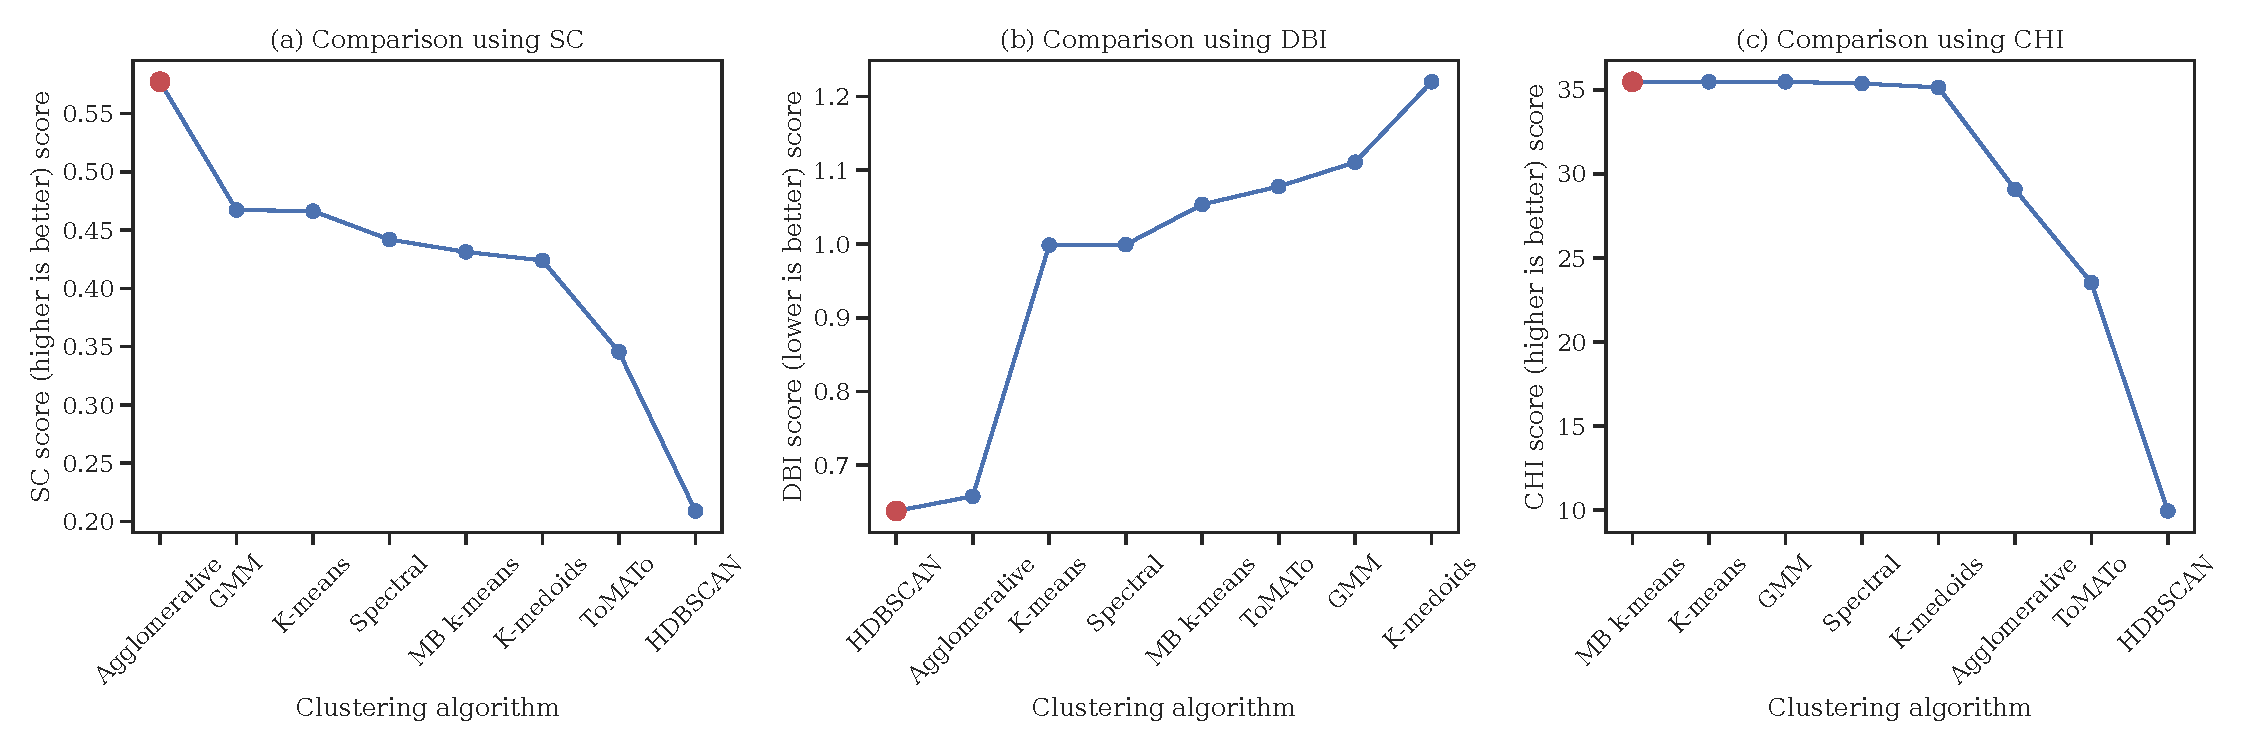
\includegraphics[width=\textwidth]{thesis/figures/cluster-analysis-numbers-word-group-internal-cluster-validation.pdf}
    \caption{Comparison of clustering algorithms trained on number word embeddings from SGNS-enwiki, ranked by internal cluster validation methods. The red dot in each plot denotes the most optimal value.}
    \label{fig:cluster-analysis-numbers-word-group-internal-cluster-validation}
\end{figure}

Furthermore, we use the agglomerative clustering algorithm. To find its best criterion and number of clusters, we first visualize its results in \cref{fig:cluster-analysis-agglomerative-numbers-word-group-internal-cluster-validation}. From \cref{fig:cluster-analysis-agglomerative-numbers-word-group-internal-cluster-validation}, we see that SC (a) prefers complete linkage criterion with 2 clusters, DBI (b) prefers single linkage criterion with 6 clusters and CHI (c) prefers ward linkage criterion with 3 clusters. In other words, we here see a different behaviour of the internal cluster validation methods than in \cref{sec:comparing-clustering-algorithms} and the country/capital cluster analysis, namely that SC prefers the least amount of clusters, DBI does not prefer the most amount of clusters and CHI does not prefer the least amount of clusters.
\begin{figure}[H]
    \centering
    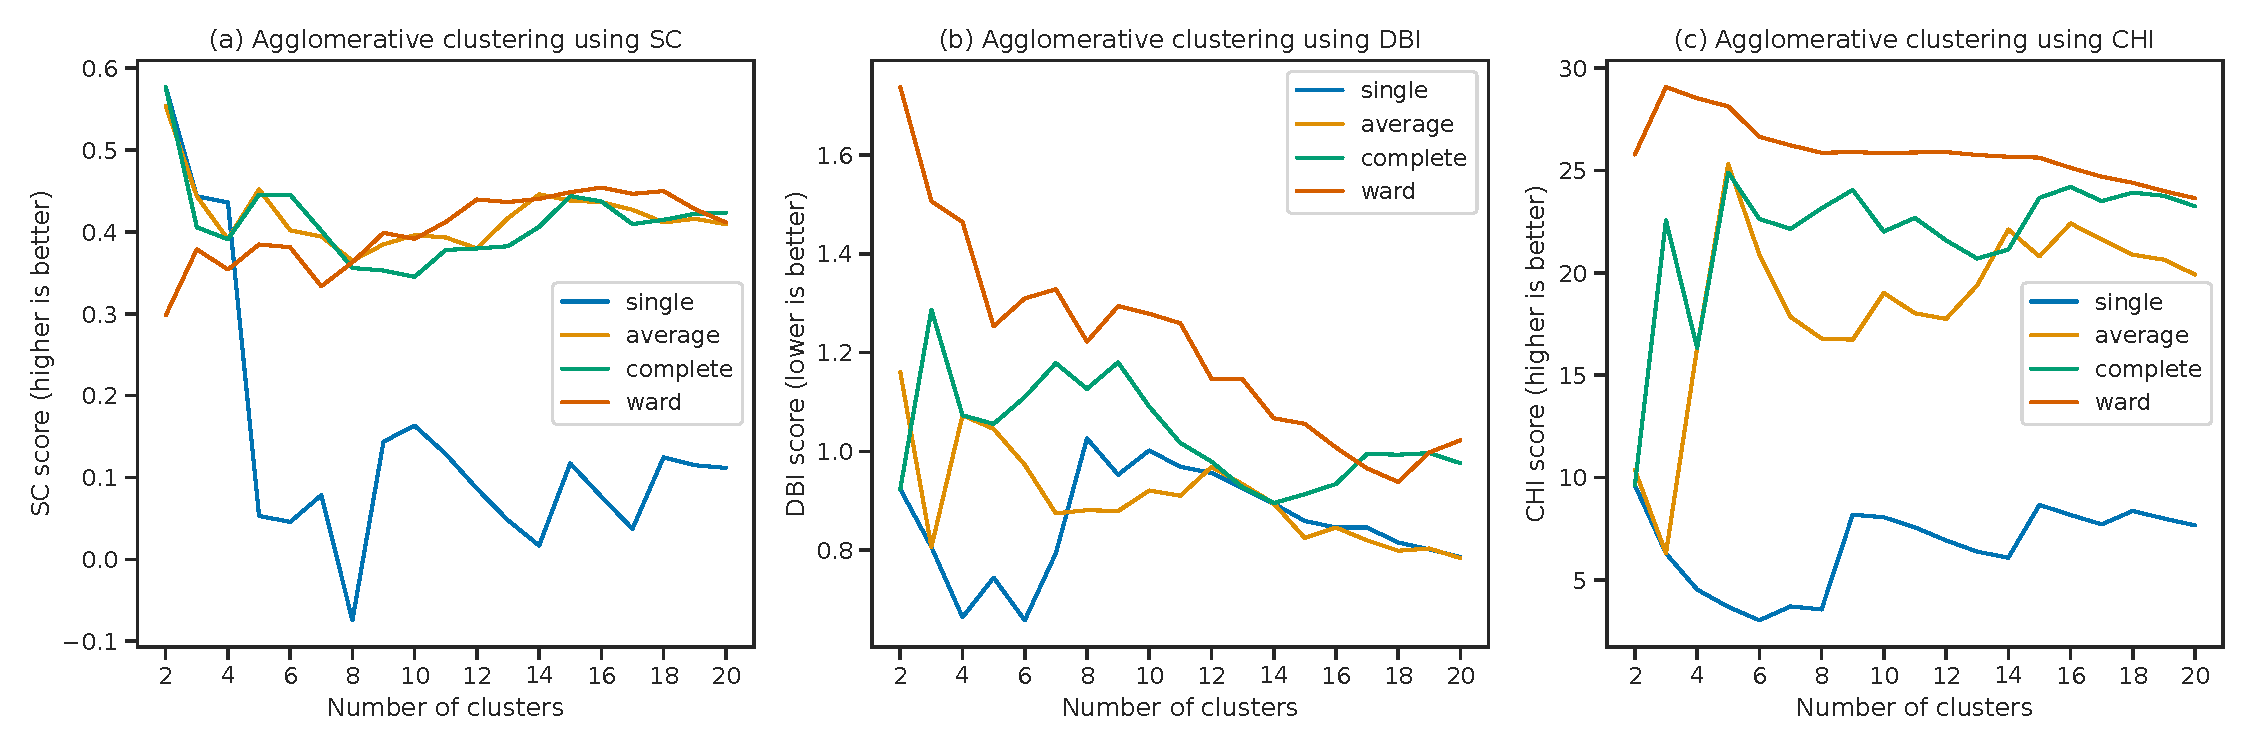
\includegraphics[width=\textwidth]{thesis/figures/cluster-analysis-agglomerative-numbers-word-group-internal-cluster-validation.pdf}
    \caption{Internal cluster validation results using agglomerative clustering on number word embeddings from SGNS-enwiki.}
    \label{fig:cluster-analysis-agglomerative-numbers-word-group-internal-cluster-validation}
\end{figure}

To understand which internal clustering validation method from \cref{fig:cluster-analysis-agglomerative-numbers-word-group-internal-cluster-validation} performs the best, we visualize the result using the best clustering of each of them in three subplots, as show in \cref{fig:cluster-analysis-agglomerative-numbers-word-group-internal-cluster-validation-best-2d-pca}. From \cref{fig:cluster-analysis-agglomerative-numbers-word-group-internal-cluster-validation-best-2d-pca}, we see that it is not entirely clear how to cluster the number word embeddings.
\begin{figure}[H]
    \centering
    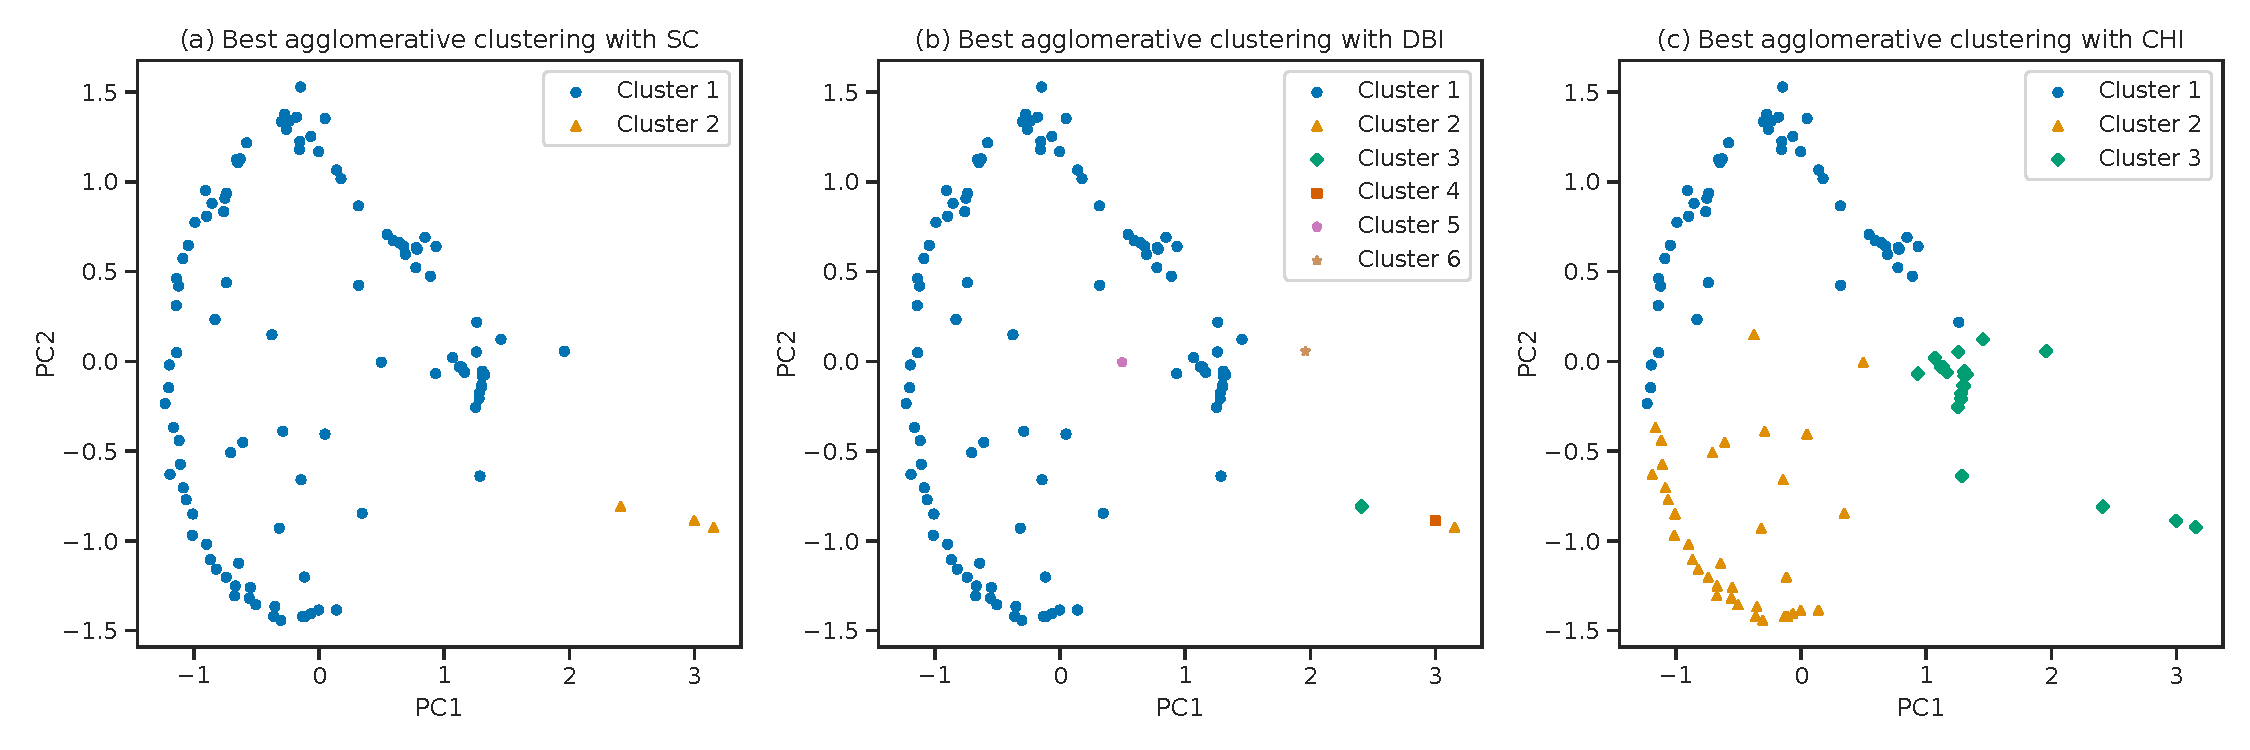
\includegraphics[width=\textwidth]{thesis/figures/cluster-analysis-agglomerative-numbers-word-group-internal-cluster-validation-best-2d-pca.pdf}
    \caption{Comparison of the best result given by internal cluster validation methods using agglomerative clustering on number word embeddings from SGNS-enwiki. Here we see that it is not clear which clustering is the best.}
    \label{fig:cluster-analysis-agglomerative-numbers-word-group-internal-cluster-validation-best-2d-pca}
\end{figure}

We further investigated the structure of the 2-dimensional PCA embedding of the number words, and noticed an interesting relationship. This relationship is illustrated in \cref{fig:ordered-number-word-embeddings-2d-pca} and shows that if we assign an increasing label from the smallest and to the largest number, we see the color of the label gradually increasing from the smallest label color to the largest label color. In other words, there seems to be an underlying sequential relationship to the word embeddings. Furthermore, this suggests that the underlying structure of number word embeddings may contain information which we have not been able to find yet.
\begin{figure}[H]
    \centering
    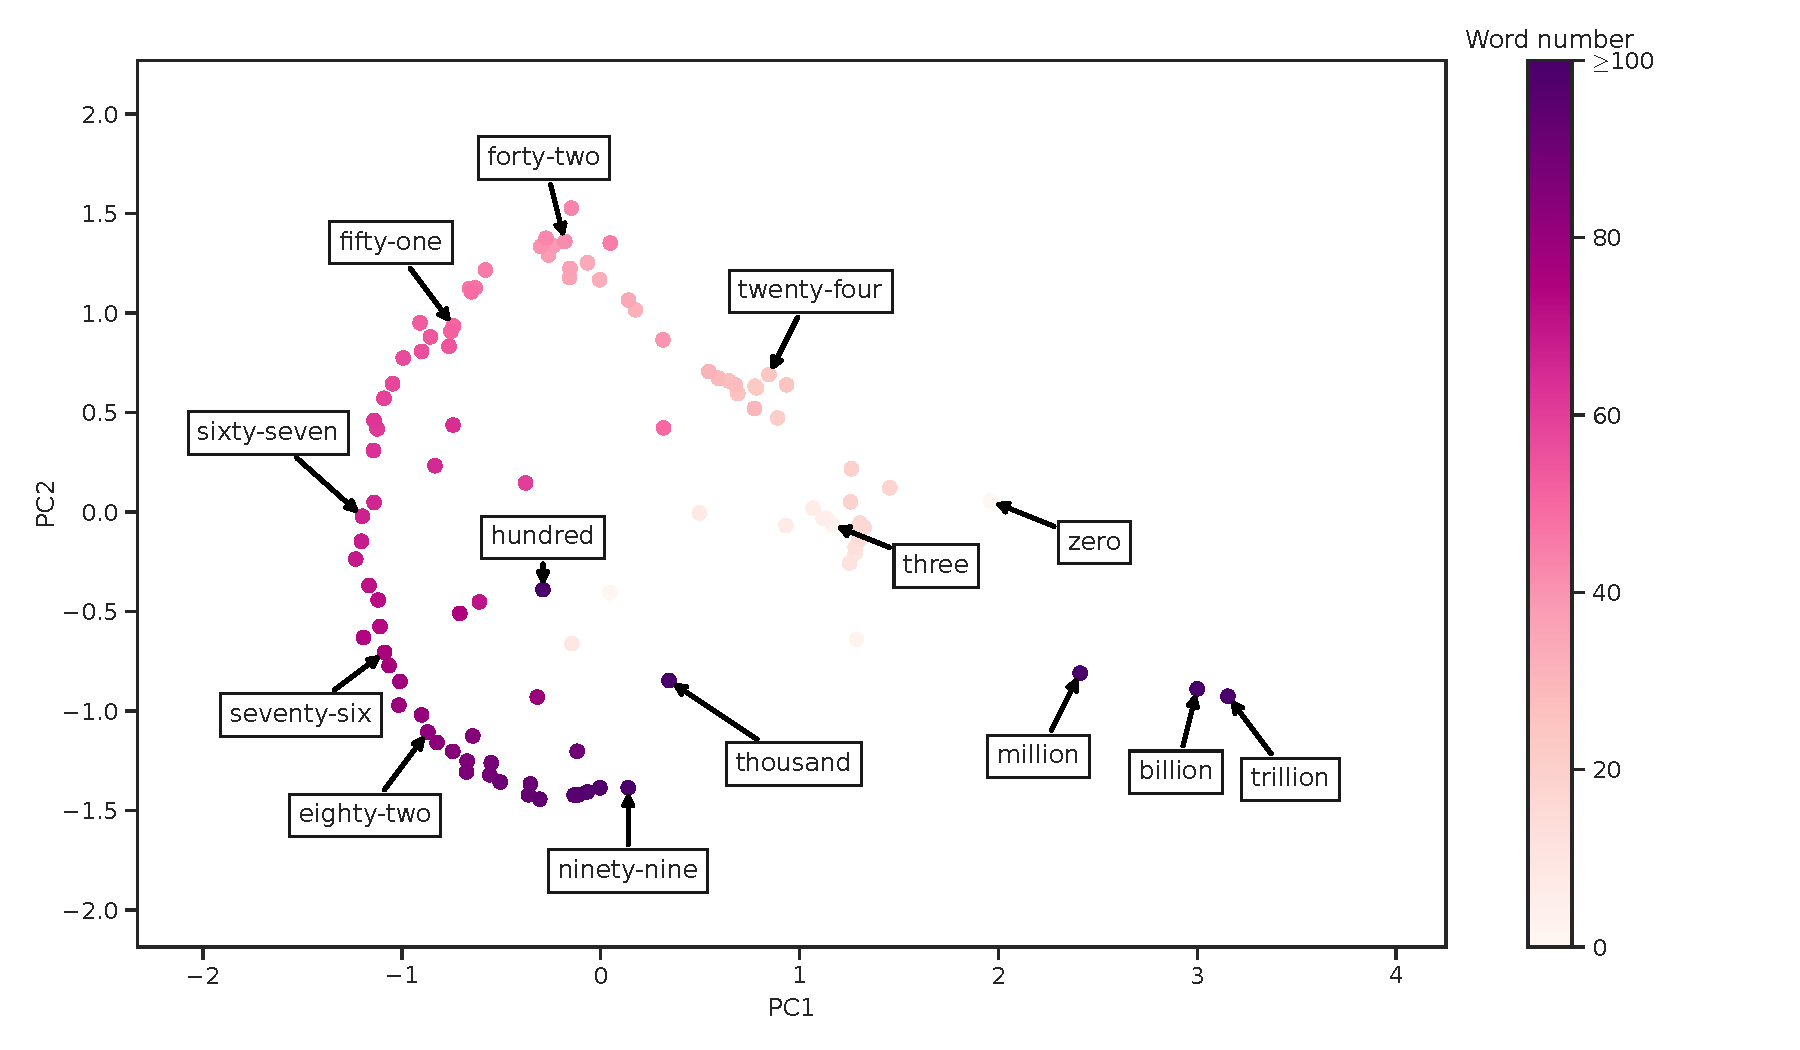
\includegraphics[width=\textwidth]{thesis/figures/ordered-number-word-embeddings-2d-pca.pdf}
    \caption{2-dimensional PCA embedding of the 105 number word embeddings, where each word embedding have an increasing label assigned to it. Here we see that as we increase the number, we see a possible underlying sequential relationship.}
    \label{fig:ordered-number-word-embeddings-2d-pca}
\end{figure}
\section{Polysemous words prediction}
\label{sec:polysemous-words-prediction}
In this section, we try to predict whether or not a word is polysemous, given its word vector. We will, first, apply methods from topological data analysis to word embeddings. In particular, we will investigate the notion of topological polysemy in \cref{sec:analysis-of-embeddings-topological-polysemy} and geometric anomaly detection in \cref{sec:analysis-of-embeddings-geometric-anomaly-detection}. We use topological polysemy to attempt to estimate the number of meanings of a word, given its word vector; we would like to see if the $\text{TPS}_n(w)$ score actually measures polysemy. In addition to this, we would like to see if singular word vectors, as identified by geometric anomaly detection, are polysemous as well. Following, we compute the estimated intrinsic dimension of word embeddings and compare the results with the number of word meanings in \cref{sec:analysis-of-embeddings-intrinsic-dimension-estimation}. Finally, we propose supervised models to predict the number of word meanings in \cref{sec:analysis-of-embeddings-supervised-polysemy-prediction}.

\subsection{Topological polysemy}
\label{sec:analysis-of-embeddings-topological-polysemy}
In this subsection, we apply topological polysemy (\cref{sec:topological-polysemy}) to the word embeddings from SGNS-enwiki. We will also train another word2vec model using the same training data used by \cite{jakubowski2020topology} and apply topological polysemy to its word embeddings. We refer to this word2vec model as the \textit{SGNS-semeval} model. Furthermore, we compare the results to topological polysemy applied to word embeddings from pre-trained models, namely the fastText model (\textit{fastText.TPS.300d}) used in experiments of \cite{jakubowski2020topology}, the \textit{GoogleNews-vectors-negative300} (shortened to \textit{GoogleNews300}) word embeddings from \cite{GoogleCodeArchiveWord2vec}, the \textit{glove.840B.300d} word embeddings from \cite{GloVeProject2014} and the English (\textit{fastText.en.300d}) word embeddings from \cite{grave2018learning}. The fastText.TPS.300d model was kindly given in private communication with one of the authors of topological polysemy \cite{ZibrowiusPrivComs2021}.

The authors of topological polysemy, \cite{jakubowski2020topology}, trained a fastText model on training data from the \textit{SemEval-2010 Task 14: Evaluation Setting for Word Sense Induction \& Disambiguation Systems} \cite{manandhar-klapaftis-2009-semeval}. The training data from the SemEval task consists of several sentences related to 100 polysemous words (50 nouns and 50 verbs). The SemEval data set also includes the number of true meanings (also called \textit{gold standard} or \textit{GS}) for each of the 100 polysemous words, as perceived by humans. In private communication with one of the authors of topological polysemy \cite{ZibrowiusPrivComs2021}, they stated that they used a fastText model with vector dimensionality of 300, and to process the training data, they removed all punctuation and replaced capital letters by the corresponding small letters. To compare with the $\text{TPS}_n(w)$, the authors use the 100 polysemous words, words from the SemEval training data which has a \textit{WordNet} \cite{fellbaum1998} entry and all words in SemEval training data. WordNet is a lexical database of the English language. In particular, it allows for querying nearly any word from the English language and and returns the \textit{synsets} of the word. Synsets of a query word $w$ is a collection of words which have similar meaning as the word $w$. In other words, by querying a word in WordNet, we can get the number of meanings of a word, as perceived by WordNet. Furthermore, the Pearson correlation coefficient \cite{James2013} is computed between $\text{TPS}_n(w)$ and GS, the number of synsets for WordNet words and the word frequency as they appear in the SemEval training data, respectively. The authors show that there is a moderate (positive) correlation between $\text{TPS}_n(w)$ and GS at $n \in \enclc{40, 50, 60}$, a decreasing correlation between $\text{TPS}_n(w)$ and the number of synsets for WordNet words and no correlation between $\text{TPS}_n(w)$ and word frequencies. In our implementation of topological polysemy, we utilized multiprocessing and the ScaNN \cite{scann2020} approximate nearest neighbour algorithm to speed up the computation. ScaNN was chosen because it performs well when applied to word embeddings, as shown in \cite{AnnBenchmarks2021}. We used the \path{ripser} \cite{ctralie2018ripser} Python package to compute Vietoris–Rips complexes. \textbf{TODO}: Ripser or Gudhi?

We trained the SGNS-semeval model using the training data from the SemEval task and the hyperparameters used to train the SGNS-enwiki model from \cref{sec:word2vec-hyperparameter-choices}. This resulted in a vocabulary size of $\sim$122K words and corpus size of $\sim$67 million for the SGNS-enwiki model. Following, we will compare the results from the experiments of \cite{jakubowski2020topology} by computing topological polysemy at varying levels of $n$ using the word embeddings of SGNS-enwiki and SGNS-semeval. Finally, we compare the results using the SGNS-enwiki and SGNS-semeval word embeddings to the word embeddings of the fastText.TPS.300d, GoogleNews300, glove.840B.300d and fastText.en.300d models.

The results of computing topological polysemy at varying levels of $n$ using the word embeddings of SGNS-enwiki and SGNS-semeval are shown in \cref{table:tps-n-correlation-sgns-enwiki,table:tps-n-correlation-sgns-semeval}. From \cref{table:tps-n-correlation-sgns-enwiki}, we see that the correlation between $\text{TPS}_n$ and GS is rather stable with respect to $n$. In particular, we notice that the correlation between $\text{TPS}_n$ and GS is negative, suggesting a relationship in the opposite direction of the results from \cite[Table 1]{jakubowski2020topology}. Nonetheless, we see a decreasing correlation when comparing $\text{TPS}_n$ versus the number of WordNet synsets for each word, and a negligible correlation between $\text{TPS}_n$ and word frequencies of the top 10000 most common words. Furthermore, from \cref{table:tps-n-correlation-sgns-semeval}, we observe a decreasing negative correlation (towards zero) between $\text{TPS}_n$ and GS, meaning that the SGNS-semeval model performs worse than the SGNS-enwiki model on this particular task. This may indicate that by training SGNS-semeval on a smaller vocabulary than the vocabulary of SGNS-enwiki we get worse results. Furthermore, we see a a decreasing correlation between $\text{TPS}_n$ and the number of WordNet synsets and a negligible correlation between $\text{TPS}_n$ and word frequencies of the top 10000 most common words. Although the negative correlation between $\text{TPS}_n$ and the number of WordNet synsets is larger for the SGNS-semeval model than the SGNS-enwiki model, it is still not particularly large. In addition to this, we are considering a lot fewer words when computing the correlation in the SGNS-semeval model than the SGNS-enwiki model (see sample size).
\begin{table}[H]
    \centering
    \begin{tabular}{@{}rrrr@{}}
    \toprule
    $n$ & $\text{TPS}_n$ vs. GS & $\text{TPS}_n$ vs. synsets & $\text{TPS}_n$ vs. frequency \\
    \midrule
    \trcolor 10  & -0.353        & -0.077             & \textbf{-0.043}               \\
    40  & \textbf{-0.383}        & -0.181             & -0.041               \\
    \trcolor 50  & -0.380        & -0.190             & -0.041               \\
    60  & -0.381        & -0.196             & -0.040               \\
    \trcolor 100 & -0.380        & \textbf{-0.205}             & -0.033               \\
    \midrule
    \textit{sample size} & 98 & 144 412 & 10 000 \\
    \bottomrule
    \end{tabular}
    \caption{Correlations between $\text{TPS}_n$ and the number of word meanings as perceived by humans (GS), the number of WordNet synsets and the word frequencies of the top 10000 most common words from the SGNS-enwiki model. \textbf{Bold} values indicate the largest (absolute) correlation.}
    \label{table:tps-n-correlation-sgns-enwiki}
\end{table}
\begin{table}[H]
    \centering
    \begin{tabular}{@{}rrrr@{}}
    \toprule
    $n$ & $\text{TPS}_n$ vs. GS & $\text{TPS}_n$ vs. synsets & $\text{TPS}_n$ vs. frequency \\
    \midrule
    \trcolor 10  & \textbf{-0.300}        & -0.248             & 0.102                \\
    40  & -0.201        & -0.300             & \textbf{0.120}                \\
    \trcolor 50  & -0.194        & -0.304             & 0.116                \\
    60  & -0.169        & -0.306             & 0.110                \\
    \trcolor 100 & -0.130        & \textbf{-0.310}             & 0.098                \\
    \midrule
    \textit{sample size} & 100 & 62 111 & 10 000 \\
    \bottomrule
    \end{tabular}
    \caption{Correlations between $\text{TPS}_n$ and the number of word meanings as perceived by humans (GS), the number of WordNet synsets and the word frequencies of the top 10000 most common words from the SGNS-semeval model. \textbf{Bold} values indicate the largest (absolute) correlation.}
    \label{table:tps-n-correlation-sgns-semeval}
\end{table}

To further broaden our understanding of the results from computing topological polysemy of the word embeddings of the SGNS-enwiki and the SGNS-semeval model, we plot $\text{TPS}_n(w)$ against the GS, the number of WordNet synsets and word frequencies, as shown in \cref{fig:tps-n-correlation-sgns-enwiki,fig:tps-n-correlation-sgns-semeval}. For each plot, we let $n$ be equal to the most optimal value for each column in \cref{table:tps-n-correlation-sgns-enwiki,table:tps-n-correlation-sgns-semeval}. From \cref{table:tps-n-correlation-sgns-enwiki}, we see a similar situation to the results from \cite[Figures 8 and 9]{jakubowski2020topology}, namely that in plot (a) we see an indication of a linear relationship between $\text{TPS}_n(w)$ and the SemEval gold standard and in plot (b) we see a clear trend between $\text{TPS}_n(w)$ and the number of synsets in WordNet. In plot (c) it is clear that there is no apparent relationship between $\text{TPS}_n(w)$ and the word frequencies. Following, we see a similar situation appearing in \cref{table:tps-n-correlation-sgns-enwiki}. These results suggest that, even by computing $\text{TPS}_n(w)$ of the SGNS-enwiki word embeddings, which has a vocabulary much larger than in the experiments of \cite{jakubowski2020topology}, we are unable to use $\text{TPS}_n(w)$ alone for predicting the number of word meanings, as given by the number of WordNet synsets.
\begin{figure}[H]
    \centering
    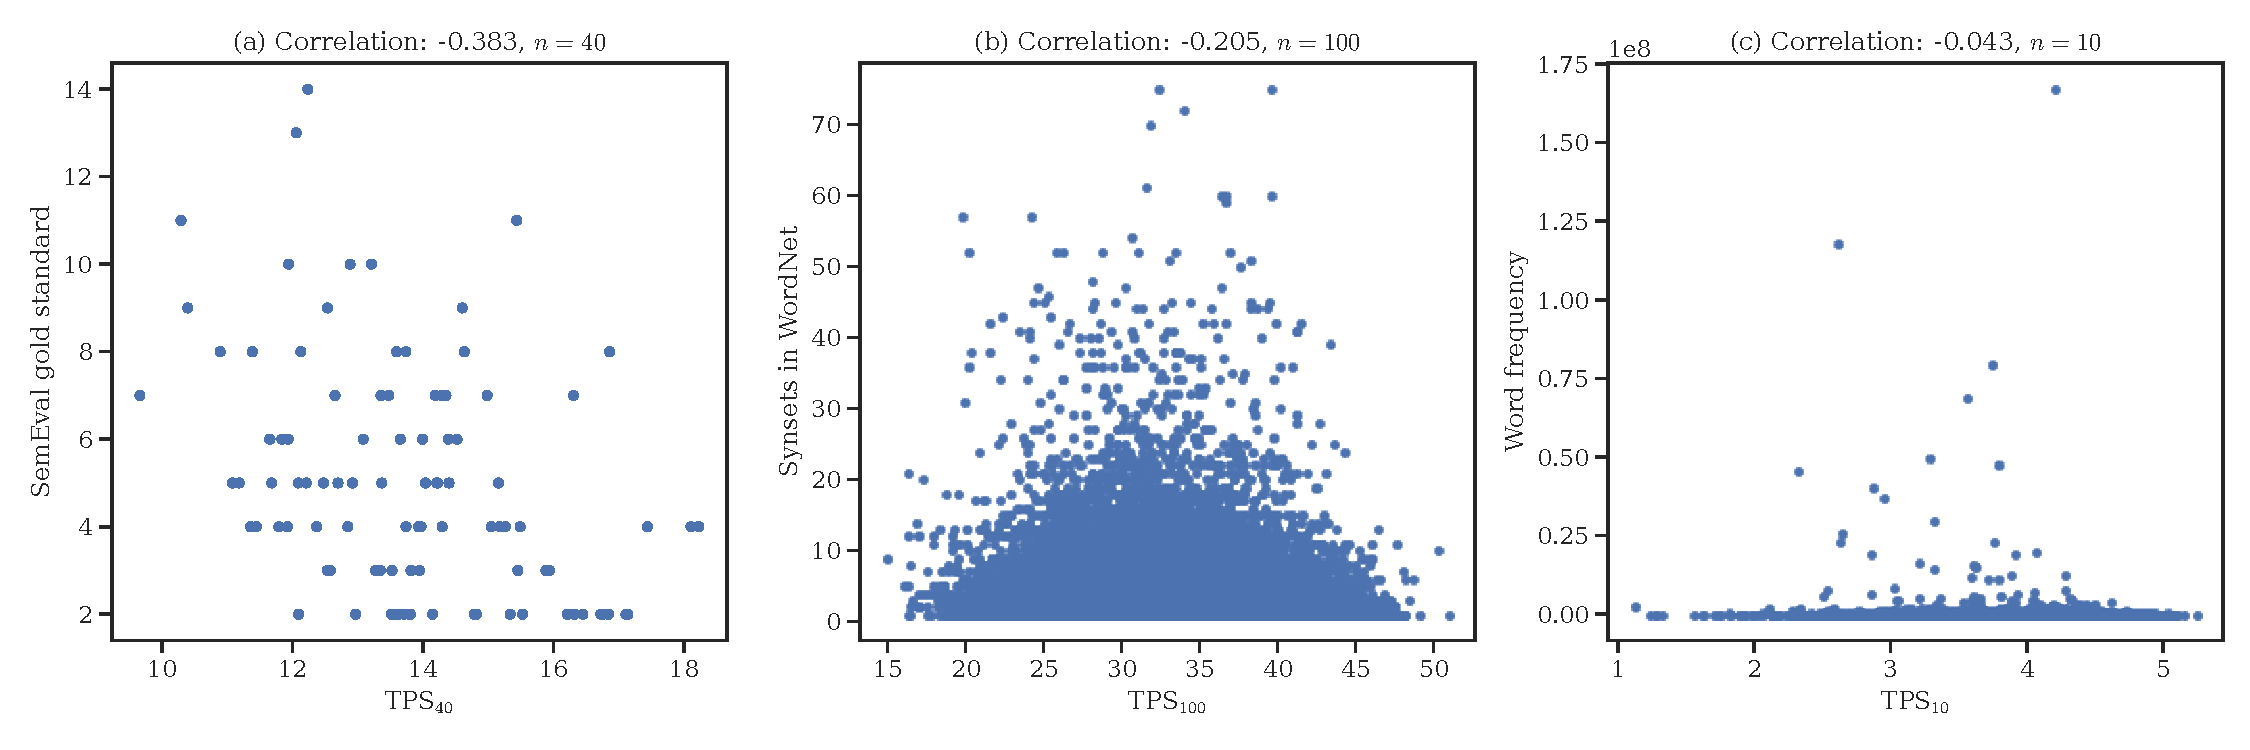
\includegraphics[width=\textwidth]{thesis/figures/tps-n-correlation-sgns-enwiki.pdf}
    \caption{Topological polysemy $\text{TPS}_n(w)$ of the word embeddings of SGNS-enwiki plotted against the GS (a), the number of WordNet synsets (b) and word frequencies (c). Plots are inspired by \cite[Figures 8 and 9]{jakubowski2020topology}.}
    \label{fig:tps-n-correlation-sgns-enwiki}
\end{figure}
\begin{figure}[H]
    \centering
    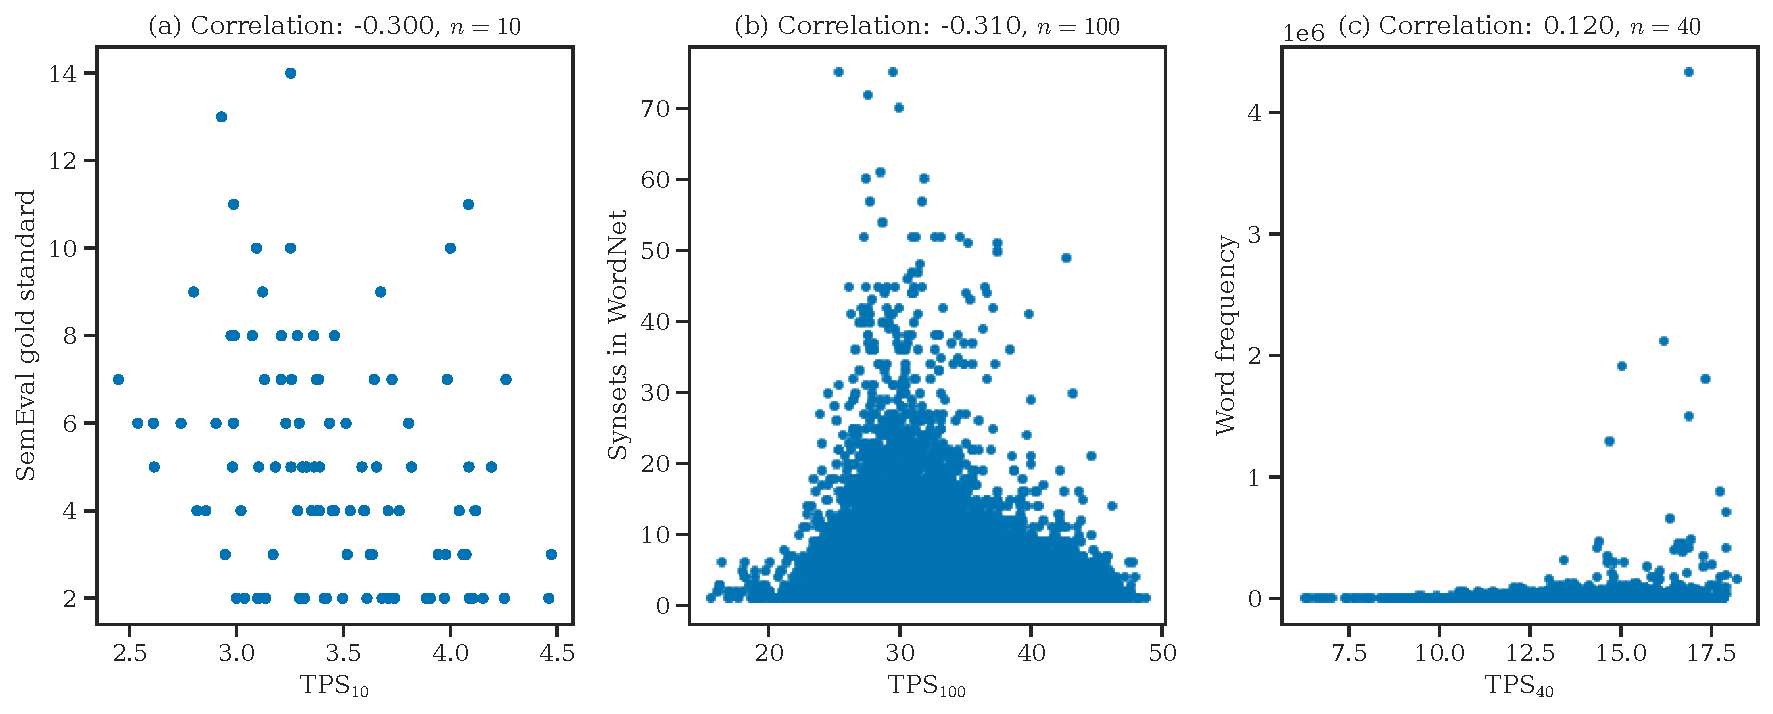
\includegraphics[width=\textwidth]{thesis/figures/tps-n-correlation-sgns-semeval_2010_task_14.pdf}
    \caption{Topological polysemy $\text{TPS}_n(w)$ of the word embeddings of SGNS-semeval plotted against the GS (a), the number of WordNet synsets (b) and word frequencies (c). Plots are inspired by \cite[Figures 8 and 9]{jakubowski2020topology}.}
    \label{fig:tps-n-correlation-sgns-semeval}
\end{figure}

Following, we compare the results of computing $\text{TPS}_n(w)$ of the word embeddings of the SGNS-enwiki and SGNS-semeval models to the word embeddings of the fastText.TPS.300d, GoogleNews300, glove.840B.300d and fastText.en.300d models. The $\text{TPS}_n(w)$ results of using the fastText.TPS.300d model are shown in \cref{table:tps-n-correlation-fasttext-tps-word-embeddings}, and using the GoogleNews300, glove.840B.300d and fastText.en.300d models are shown in \cref{table:tps-n-correlation-external-word-embeddings}. We do not compute the correlation between $\text{TPS}_n(w)$ and word frequencies in \cref{table:tps-n-correlation-fasttext-tps-word-embeddings,table:tps-n-correlation-external-word-embeddings}, since we do not have the data available. In addition to this, it is unlikely that $\text{TPS}_n(w)$ and word frequencies have anything in common, as show in the previous results using the SGNS-enwiki and SGNS-semeval models, as well as by the experiments of \cite{jakubowski2020topology}. From \cref{table:tps-n-correlation-fasttext-tps-word-embeddings}, we see similar results to the experiments of \cite{jakubowski2020topology}, namely that we get a modest, positive correlation when comparing $\text{TPS}_n(w)$ to the SemEval gold standard, and that we get a decreasing correlation when comparing $\text{TPS}_n(w)$ to the number of WordNet synsets. We note, however, that we do not get the exact same correlation results as \cite{jakubowski2020topology}; this could be affected by the use of ScaNN to approximate the nearest neighbours. Furthermore, from \cref{table:tps-n-correlation-external-word-embeddings} we see that the GoogleNews300 models yields particularly high values when comparing $\text{TPS}_n(w)$ to the SemEval gold standard, while the remaining models are modest at best. We also observe that when comparing $\text{TPS}_n(w)$ to the number of WordNet synsets, we do not get high correlation scores. This further suggests that by only increasing the vocabulary of the word embedding model, we are not able to model the number of WordNet synsets very well, by only using the $\text{TPS}_n(w)$ scores. Additionally, the correlation results shown in \cref{table:tps-n-correlation-external-word-embeddings} indicate that the $\text{TPS}_n(w)$ scores are behaving rather inconsistent across the data sets, and it is not clear if $\text{TPS}_n(w)$ measures polysemy of words.
\begin{table}[H]
    \centering
    \begin{tabular}{@{}rrr@{}}
    \toprule
    $n$ & $\text{TPS}_n$ vs. GS & $\text{TPS}_n$ vs. synsets \\
    \midrule
    \trcolor 10 & 0.131	& \textbf{0.135} \\
    40 & 0.395 & 0.066 \\
    \trcolor 50 & \textbf{0.416} & 0.053 \\
    60 & 0.363 & 0.043 \\
    \trcolor 100 & 0.301 & 0.020 \\
    \midrule
    \textit{sample size} & 100 & 62 049 \\
    \bottomrule
    \end{tabular}
    \caption{Correlations between $\text{TPS}_n$ and the number of word meanings as perceived by humans (GS) and the number of WordNet synsets from the fastText.TPS.300d model. \textbf{Bold} values indicate the largest (absolute) correlation.}
    \label{table:tps-n-correlation-fasttext-tps-word-embeddings}
\end{table}
\begin{table}[H]
    \centering
    \begin{tabular}{ccccccc}
    \toprule
    \multicolumn{1}{c}{\multirow{2}{*}{$n$}} & \multicolumn{2}{c}{GoogleNews300}    & \multicolumn{2}{c}{glove.840B.300d}              & \multicolumn{2}{c}{fastText.en.300d}             \\
    \cmidrule(l){2-7} 
    \multicolumn{1}{c}{}                   & \makecell[tc]{$\text{TPS}_n$ vs.\\GS} & \makecell[tc]{$\text{TPS}_n$ vs.\\synsets} & \makecell[tc]{$\text{TPS}_n$ vs.\\GS} & \makecell[tc]{$\text{TPS}_n$ vs.\\synsets} & \makecell[tc]{$\text{TPS}_n$ vs.\\GS} & \makecell[tc]{$\text{TPS}_n$ vs.\\synsets} \\ \midrule
    \trcolor 10           & \textbf{-0.446}  & -0.095       & -0.103  & 0.008        & -0.240  & \textbf{0.114}        \\
    40           & \textbf{-0.446}  & -0.166       & \textbf{-0.125}  & -0.039       & \textbf{-0.289}  & 0.110        \\
    \trcolor 50           & -0.436  & -0.174       & -0.053  & -0.044       & -0.199  & 0.108        \\
    60           & -0.428  & -0.180       & -0.023  & -0.048       & -0.150  & 0.105        \\
    \trcolor 100          & -0.417  & \textbf{-0.193}       & -0.053  & \textbf{-0.058}       & -0.105  & 0.099        \\
    \midrule
    \makecell[tc]{\textit{sample}\\\textit{size}} & 100 & 207 119 & 100 & 249 352 & 100 & 230 175 \\
    \bottomrule
    \end{tabular}
    \caption{Correlations between $\text{TPS}_n$ and the number of word meanings as perceived by humans (GS), and the number of WordNet synsets from the GoogleNews300, glove.840B.300d and fastText.en.300d models. \textbf{Bold} values indicate the largest (absolute) correlation.}
    \label{table:tps-n-correlation-external-word-embeddings}
\end{table}

To compare how well the various word embedding models agree on the $\text{TPS}_n(w)$, we will create a correlation matrix by comparing $\text{TPS}_n(w)$ and the SemEval gold standard. Using a correlation matrix, we summarize the results nicely and further deepen our understanding of the results. By majority vote, we will let $n=40$ when comparing $\text{TPS}_n(w)$ and the SemEval gold standard. The correlation matrix is shown in \cref{fig:correlation-matrix-tps-vs-gs}. From \cref{fig:correlation-matrix-tps-vs-gs}, we see that the SGNS-enwiki, SGNS-semeval and GoogleNews300 models yield similar $\text{TPS}_{40}(w)$ results. We also note that the fastText.TPS.300d model either yield no correlation (approximately equal to zero) or negative correlations, when compared to the other models.
\begin{figure}[H]
    \centering
    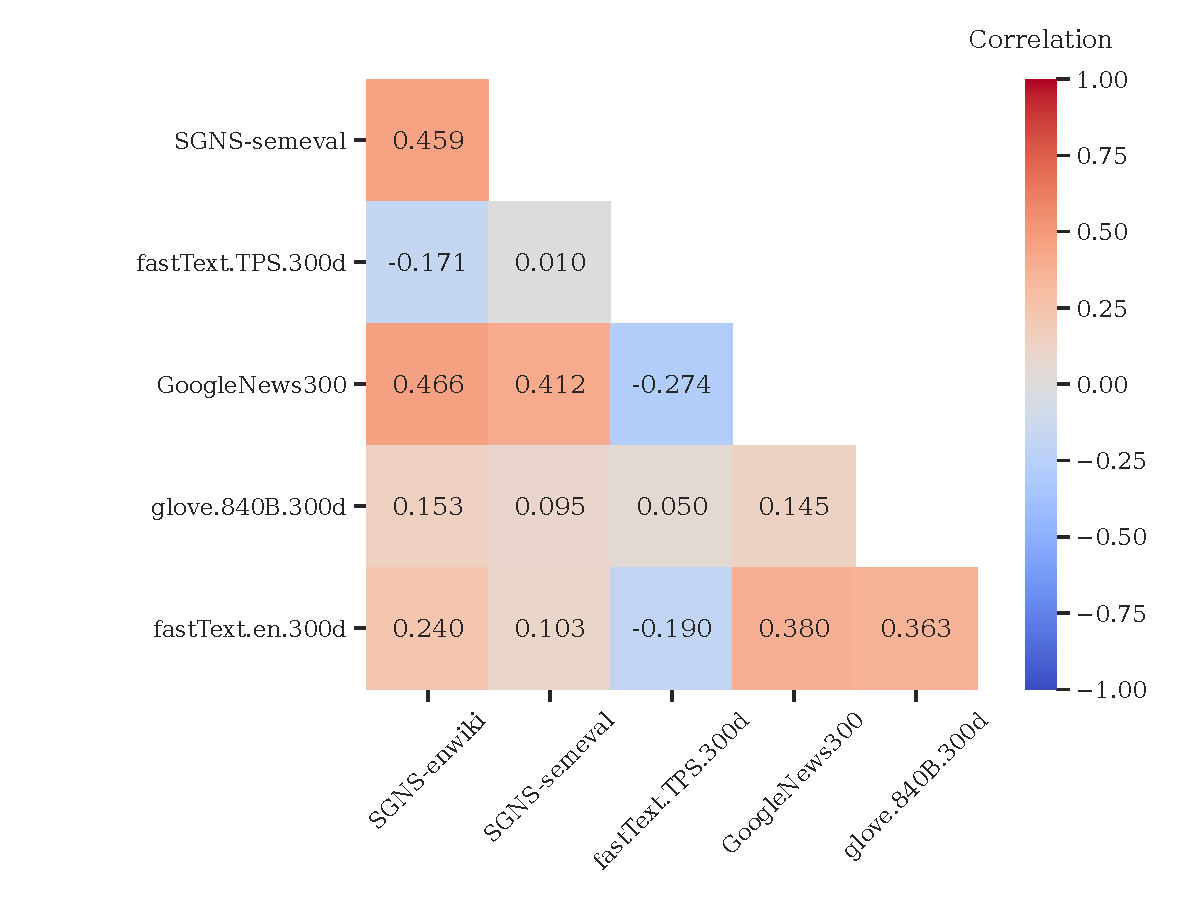
\includegraphics[width=0.8\textwidth]{thesis/figures/correlation-matrix-tps-vs-gs.pdf}
    \caption{Correlation matrix between for comparing word embedding models on correlations between $\text{TPS}_{40}(w)$ and the SemEval gold standard. High (absolute) values indicate that the two models are similar in terms of scoring using $\text{TPS}_{40}(w)$.}
    \label{fig:correlation-matrix-tps-vs-gs}
\end{figure}

To deepen the understanding, we visualize the similarity of the SGNS-enwiki, SGNS-semeval and GoogleNews300 models in \cref{fig:tps-vs-gs-top-3-correlation-word-embedding-models}, where we can see linear relationships appearing. These results suggest that the SGNS-enwiki, SGNS-semeval and GoogleNews300 models agree on how to score using $\text{TPS}_{40}(w)$.
\begin{figure}[H]
    \centering
    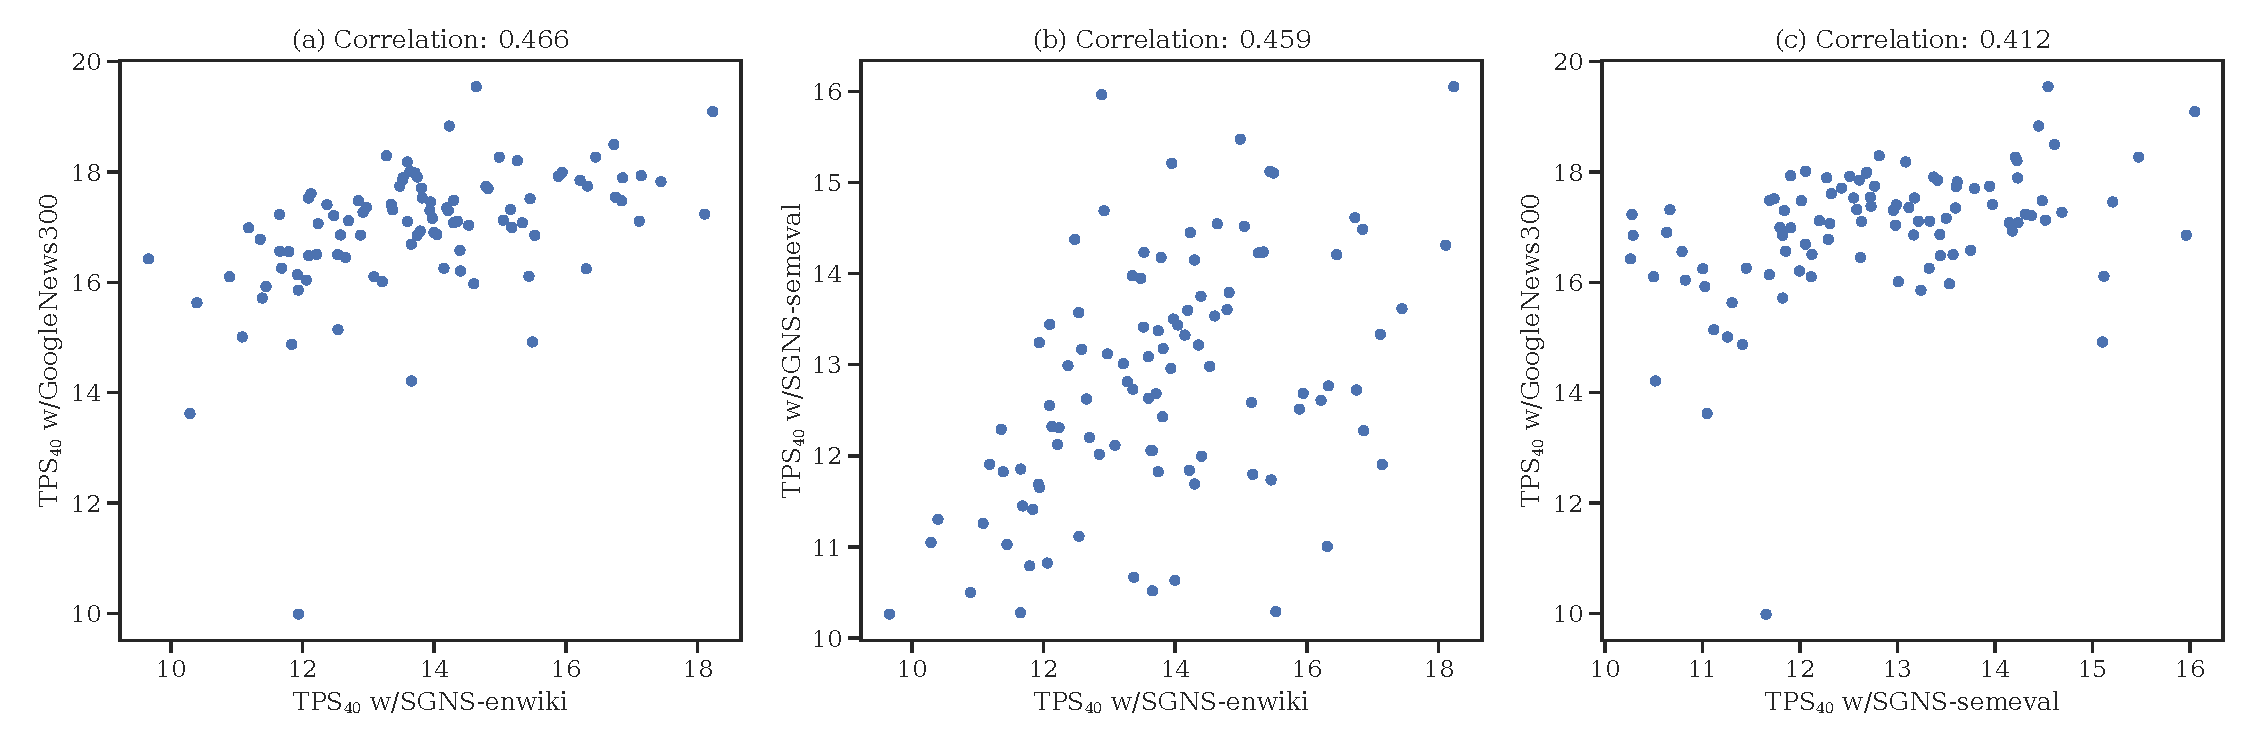
\includegraphics[width=\textwidth]{thesis/figures/tps-vs-gs-top-3-correlation-word-embedding-models.pdf}
    \caption{$\text{TPS}_{40}(w)$ scores plotted against each other using the SGNS-enwiki, SGNS-semeval and GoogleNews300 models.}
    \label{fig:tps-vs-gs-top-3-correlation-word-embedding-models}
\end{figure}

Following, we look at the three negative correlations from \cref{fig:correlation-matrix-tps-vs-gs} and visualize the negative relationships in \cref{fig:tps-vs-gs-top-3-negative-correlation-word-embedding-models}. From \cref{fig:tps-vs-gs-top-3-negative-correlation-word-embedding-models}, we see negative relationships appearing, although it is less significant than the positive relationships seen in \cref{fig:tps-vs-gs-top-3-correlation-word-embedding-models}.
\begin{figure}[H]
    \centering
    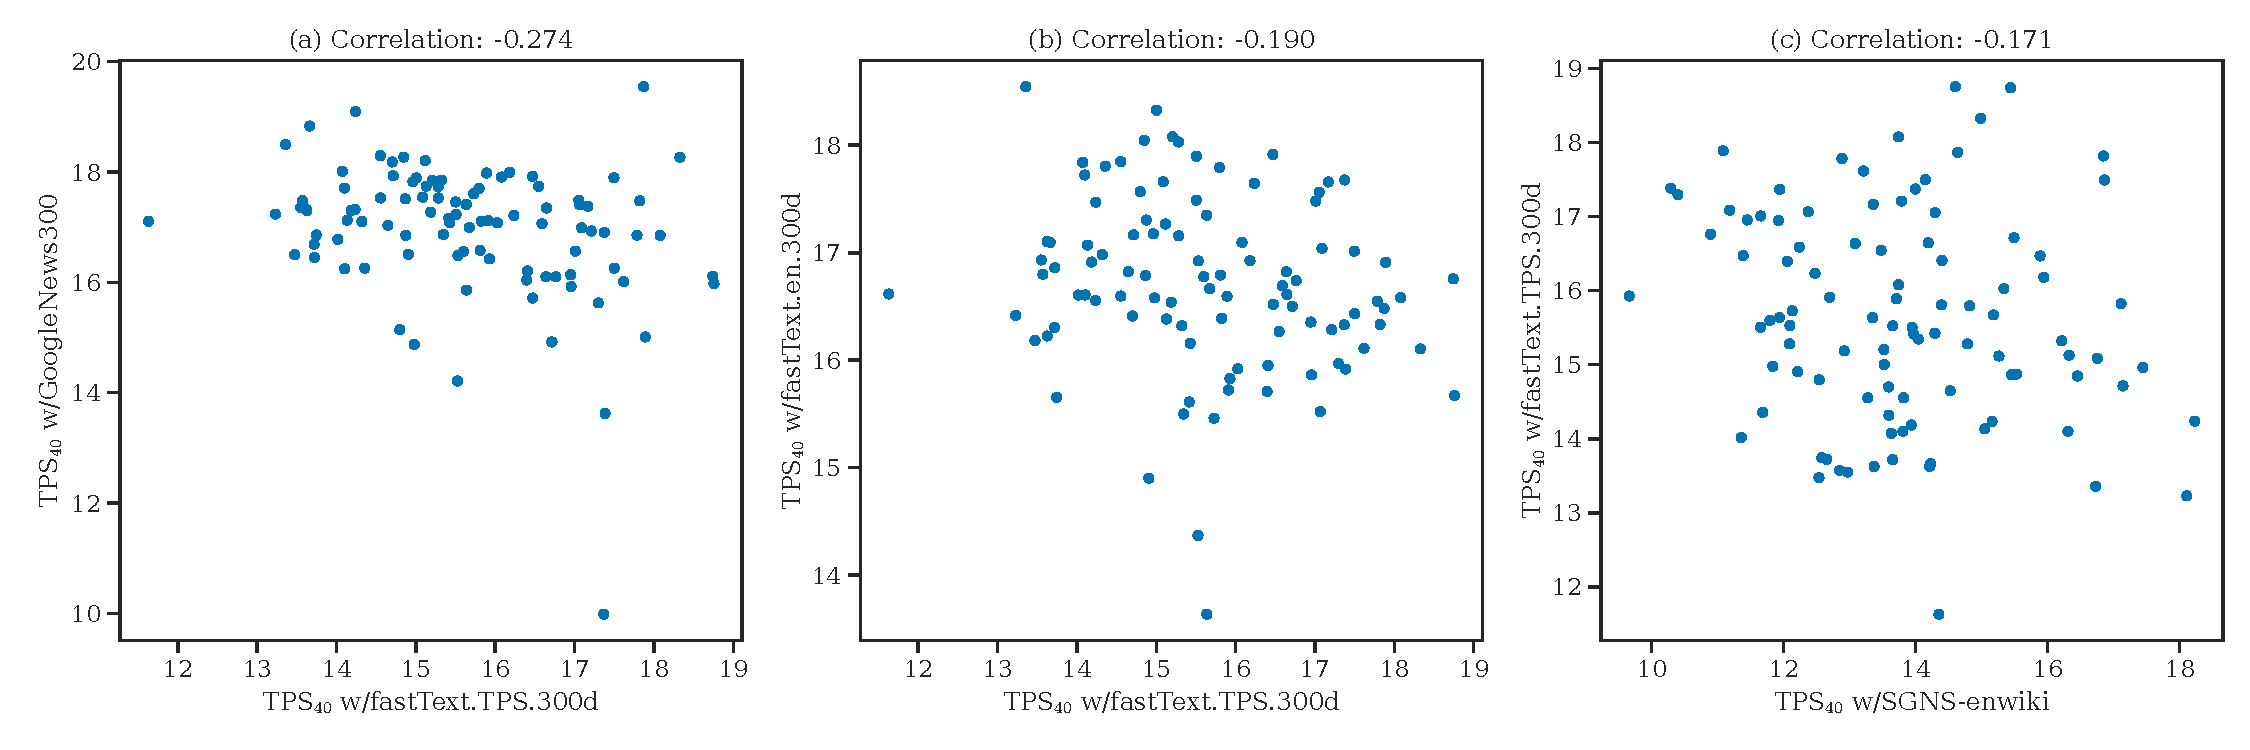
\includegraphics[width=\textwidth]{thesis/figures/tps-vs-gs-top-3-negative-correlation-word-embedding-models.pdf}
    \caption{$\text{TPS}_{40}(w)$ scores plotted against each other using the fastText.TPS.300d, GoogleNews300, fastText.en.300d and SGNS-enwiki models.}
    \label{fig:tps-vs-gs-top-3-negative-correlation-word-embedding-models}
\end{figure}

We have now looked at the effect of computing $\text{TPS}_n(w)$ at varying levels of $n$ using various word embeddings. We saw that, even by decreasing/increasing the vocabulary size of the word embedding models, the $\text{TPS}_n(w)$ score did not improve significantly. In all our experiments (except using the fastText.TPS.300d model), the correlation between $\text{TPS}_n(w)$ and the SemEval gold standard were always negative, while in the experiments of \cite{jakubowski2020topology}, they got a moderate, positive correlation. This suggests that the topological polysemy scoring could be affected by choice of word embedding model (i.e. choosing fastText over word2vec) and the fact that the model used in \cite{jakubowski2020topology} was trained on a data set which is strongly related to the 100 polysemous words. In other words, it could seem that the measure of topological polysemy does not work well, for a general word embedding model.

To deepen our understanding of how the $\text{TPS}_n(w)$ is computed, we will perform an experiment by computing $\text{TPS}_n(w)$ of a custom data set. The custom data set consists of sampled data points of two spheres which share one intersection point. We denote this data set as \textit{2Spheres-$d$}, where $d$ represents the dimensionality of the spheres. In particular, we let $d \in \enclc{2, 3, 4, 5, 10, 20, 50, 300}$. To ensure that the dimensionality of the \textit{2Spheres-$d$} data set is similar to the dimensionality of word embeddings, we let the dimensionality of the space be equal to 300, i.e. \textit{2Spheres-$d$} $\in \R^{300}$. In other words, if $d$ was less than 300, we simply add zeros to the remaining dimensions to fill up to 300. For each sphere in \textit{2Spheres-$d$}, we generate 1000000 points on the sphere in $\R^d$. We sort the points by distance to the intersection point and further split the points into 20 intervals, i.e. chunks of 100000 data points for each sphere. Next, we sample 1000 points from each interval, leading to 20000 points for each sphere. The motivation for sampling from distance sorted intervals is to reduce the effect of the curse of dimensionality, namely that it becomes harder to measure the distance between points in high (e.g. 300) dimension. For the sake of simplicity, we let $n=50$ when computing the topological polysemy. We illustrate the result of computing $\text{TPS}_{50}$ of 2Spheres-$2$ and 2Spheres-$3$ in \cref{fig:two-spheres-2d-3d-tps-scores}. From \cref{fig:two-spheres-2d-3d-tps-scores}, we see that for both 2Spheres-$2$ and 2Spheres-$3$, the $\text{TPS}_{50}$ is at its highest (yellow color) around the intersection point between the two spheres (see plots (b) and (d)). In addition to this, at the intersection point between the two spheres, the $\text{TPS}_{50}$ score is low. These two observations suggest that, for low values of $d$, $\text{TPS}_{50}$ fails to identify the singular point, but rather manages to identify the area around it. We will now look at how the $\text{TPS}_{50}$ score behaves for $d \in \enclc{4, 5, 10, 20, 50, 300}$.
\begin{figure}[H]
    \centering
    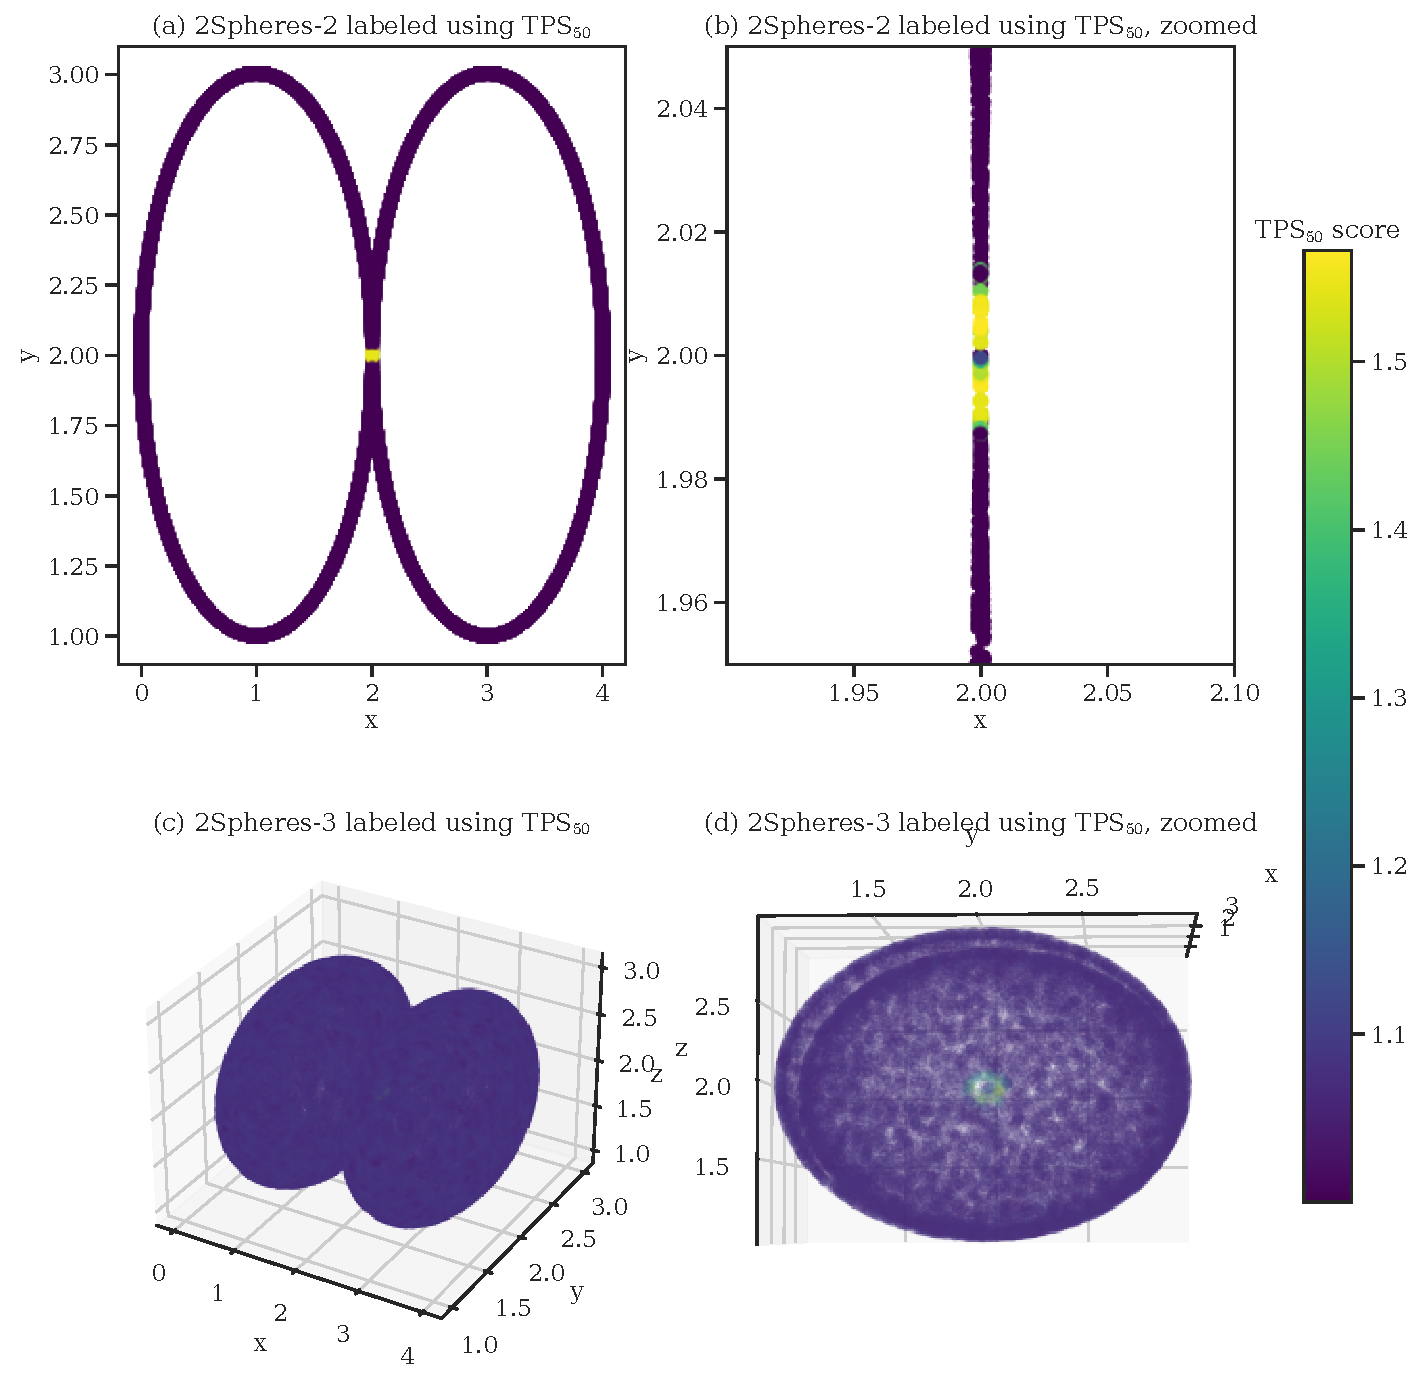
\includegraphics[width=\textwidth]{thesis/figures/two-spheres-2d-3d-tps-scores.pdf}
    \caption{Plots of the 2Spheres-$2$ and 2Spheres-$3$ data sets, with $\text{TPS}_{50}$ as labels.}
    \label{fig:two-spheres-2d-3d-tps-scores}
\end{figure}

We visualize the result of computing $\text{TPS}_{50}$ for 2Spheres-$d$ for $d \in \enclc{4, 5, 10, 20, 50, 300}$ in \cref{fig:two-spheres-distance-to-int-point-vs-tps-scores}, by plotting the distance to intersection point between the spheres against the $\text{TPS}_{50}$ score. From \cref{fig:two-spheres-distance-to-int-point-vs-tps-scores}, we see that as the dimension of the spheres increases, the "peak" of $\text{TPS}_{50}$ shown in plot (a) diminishes. The diminishing effect comes due to the curse of dimensionality (\cref{fig:curse-of-dimensionality}), namely that in high dimensional space, all distances become very similar (as seen in plot (f)). In other words, for high dimensional spheres, it becomes very hard to identify the intersection point using $\text{TPS}_{50}$, as the distances become similar, and $\text{TPS}_{50}$ is unable to identify areas around the intersection point, as we saw happened in lower dimensions (\cref{fig:two-spheres-2d-3d-tps-scores}). It should be noted, however, that for high values of $d$, the intersection point has a $\text{TPS}_{50}$ score which generally is higher than all other values of $\text{TPS}_{50}$. Finally, we argue that these results shown in \cref{fig:two-spheres-distance-to-int-point-vs-tps-scores} may indicate that the topological measure of polysemy may suffer when applied to high-dimensional (e.g. 300) data.
\begin{figure}[H]
    \centering
    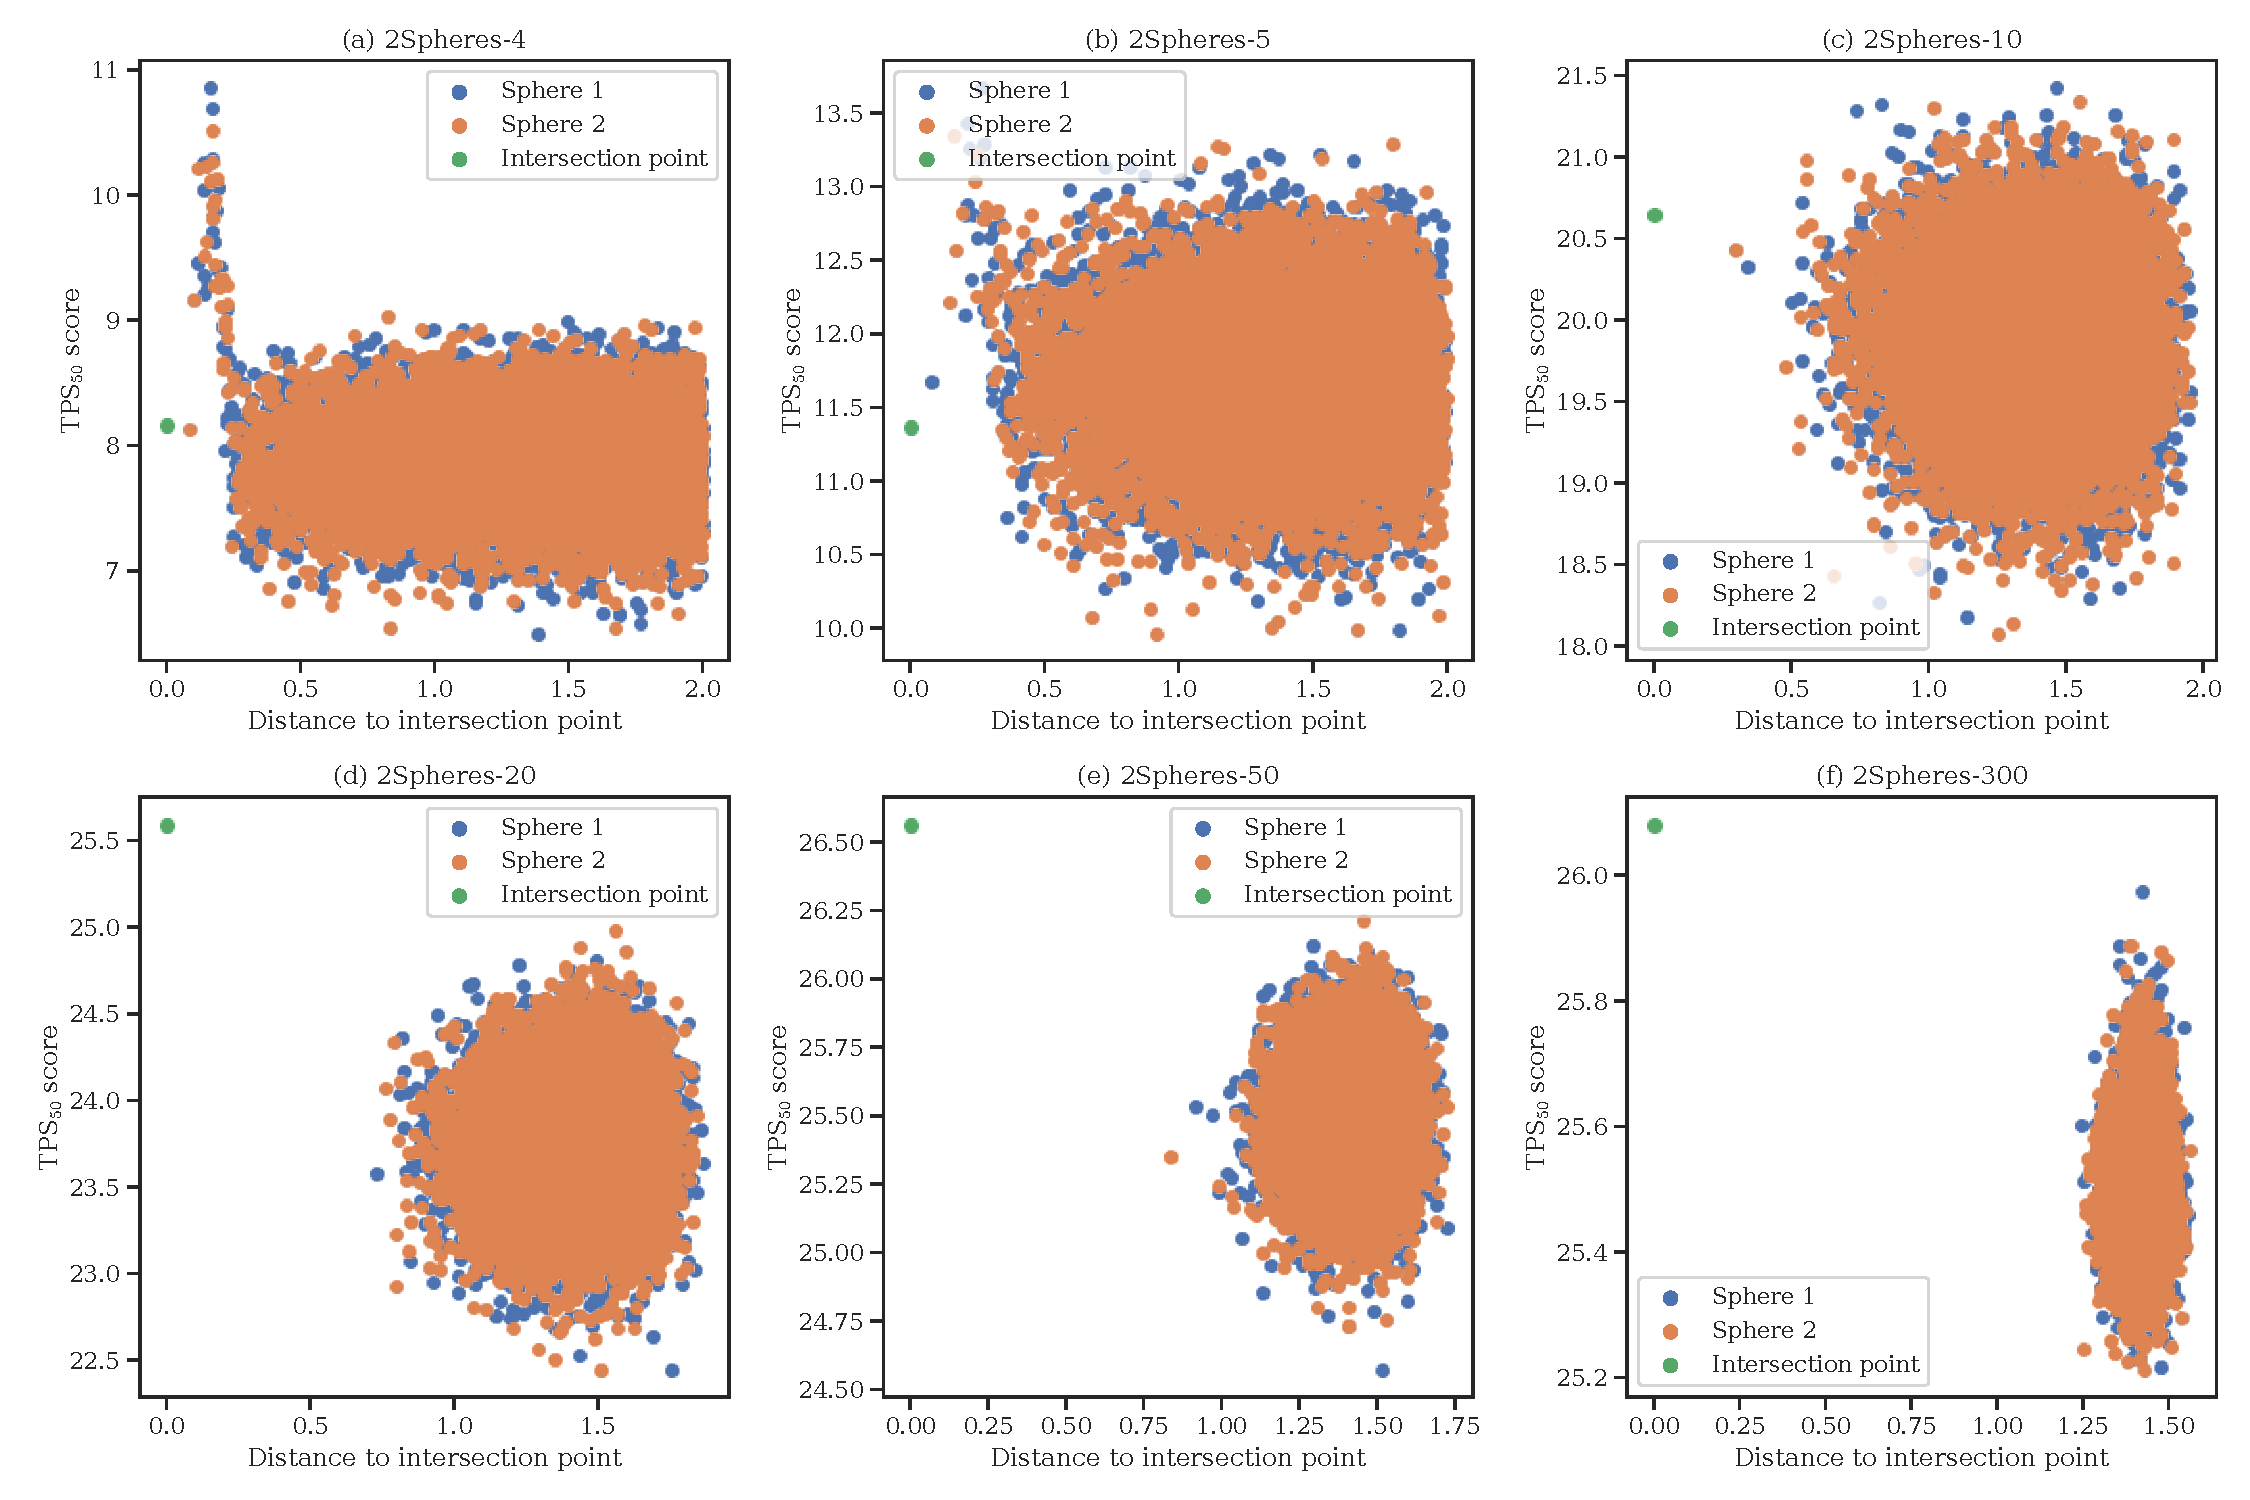
\includegraphics[width=\textwidth]{thesis/figures/two-spheres-distance-to-int-point-vs-tps-scores.pdf}
    \caption{Distance to intersection point between spheres plotted against $\text{TPS}_{50}$ score for 2Spheres-$d$, $d \in \enclc{4, 5, 10, 20, 50, 300}$.}
    \label{fig:two-spheres-distance-to-int-point-vs-tps-scores}
\end{figure}

We repeated the experiment of computing topological polysemy ($\text{TPS}_{50}$ in particular) of two spheres using a noisy version of the 2Spheres-$d$ data set, which we called the \textit{2SpheresNoisy-$d$} data set. The motivation for adding some noise to the spheres data set was to emulate some real-word effect, namely that data sets are usually not uniformly distributed in practice. In particular, the 2SpheresNoisy-$d$ data set was created by perturbing the 2Spheres-$d$ data set by adding Gaussian noise at every data point. We used Gaussians with zero mean and variance equal to 0.1 to create the noise. Following, we first computed the $\text{TPS}_{50}$ score of the 2SpheresNoisy-$2$ and 2SpheresNoisy-$3$ data sets. The results of are shown in \cref{fig:two-spheres-noisy-2d-3d-tps-scores}, where we see that in the 2-dimensional case (a), the $\text{TPS}_{50}$ scores are high (i.e. yellow color) and we are unable to identify the intersection point between the spheres. Moreover, we see in the plots on the bottom (c and d) of \cref{fig:two-spheres-noisy-2d-3d-tps-scores} that the $\text{TPS}_{50}$ scores are mediocre at best, and we are unable to identify the intersection point between the spheres. The results shown in \cref{fig:two-spheres-noisy-2d-3d-tps-scores} tells us that if we perturb the data set by adding noise, it becomes harder to identify singular points in lower dimensions ($d \in \enclc{2, 3}$), when compared to the $\text{TPS}_{50}$ results using 2Spheres-$d$, as shown in \cref{fig:two-spheres-2d-3d-tps-scores}.
\begin{figure}[H]
    \centering
    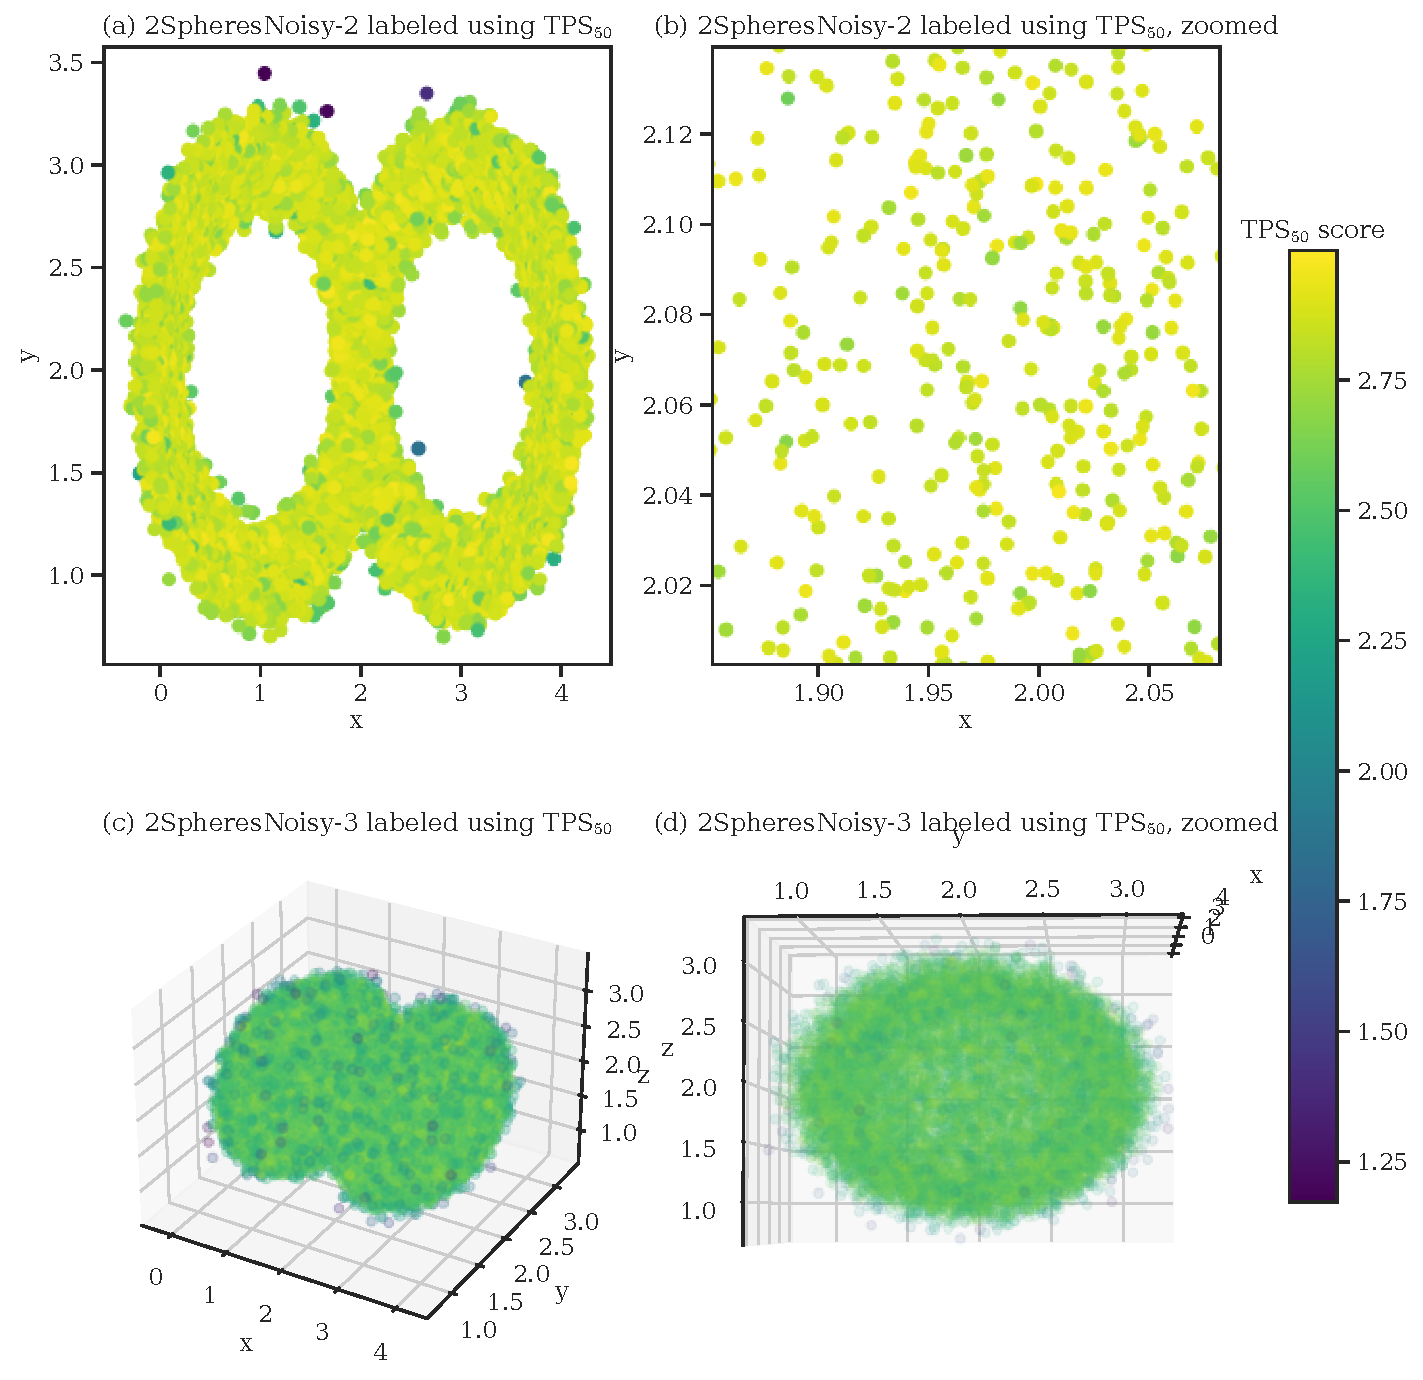
\includegraphics[width=\textwidth]{thesis/figures/two-spheres-noisy-2d-3d-tps-scores.pdf}
    \caption{Plots of the 2SpheresNoisy-$2$ and 2SpheresNoisy-$3$ data sets, with $\text{TPS}_{50}$ as labels.}
    \label{fig:two-spheres-noisy-2d-3d-tps-scores}
\end{figure}

Following, we visualize the result of computing $\text{TPS}_{50}$ for 2SpheresNoisy-$d$ for $d \in \enclc{4, 5, 10, 20, 50, 300}$ in \cref{fig:two-spheres-noisy-distance-to-int-point-vs-tps-scores}, by plotting the distance to intersection point between the spheres against the $\text{TPS}_{50}$ score. In \cref{fig:two-spheres-noisy-distance-to-int-point-vs-tps-scores}, we see a similar situation appearing when compared to the results using 2Spheres-$d$ in \cref{fig:two-spheres-distance-to-int-point-vs-tps-scores}. In particular, we observe that as we increase the dimensionality of the spheres towards 300, the distances to the intersection point become more or less the same, and it is hard to differentiate between the intersection point and regular points on the two spheres. We note, however, that in the last plot (f) in \cref{fig:two-spheres-noisy-distance-to-int-point-vs-tps-scores}, we see that the $\text{TPS}_{50}$ score is significantly larger than the rest of the $\text{TPS}_{50}$ scores, meaning that it could be possible to identify the intersection point using its $\text{TPS}_{50}$ score in this case, but we argue that this might be due to a random effect of the 2SpheresNoisy-300 data set.
\begin{figure}[H]
    \centering
    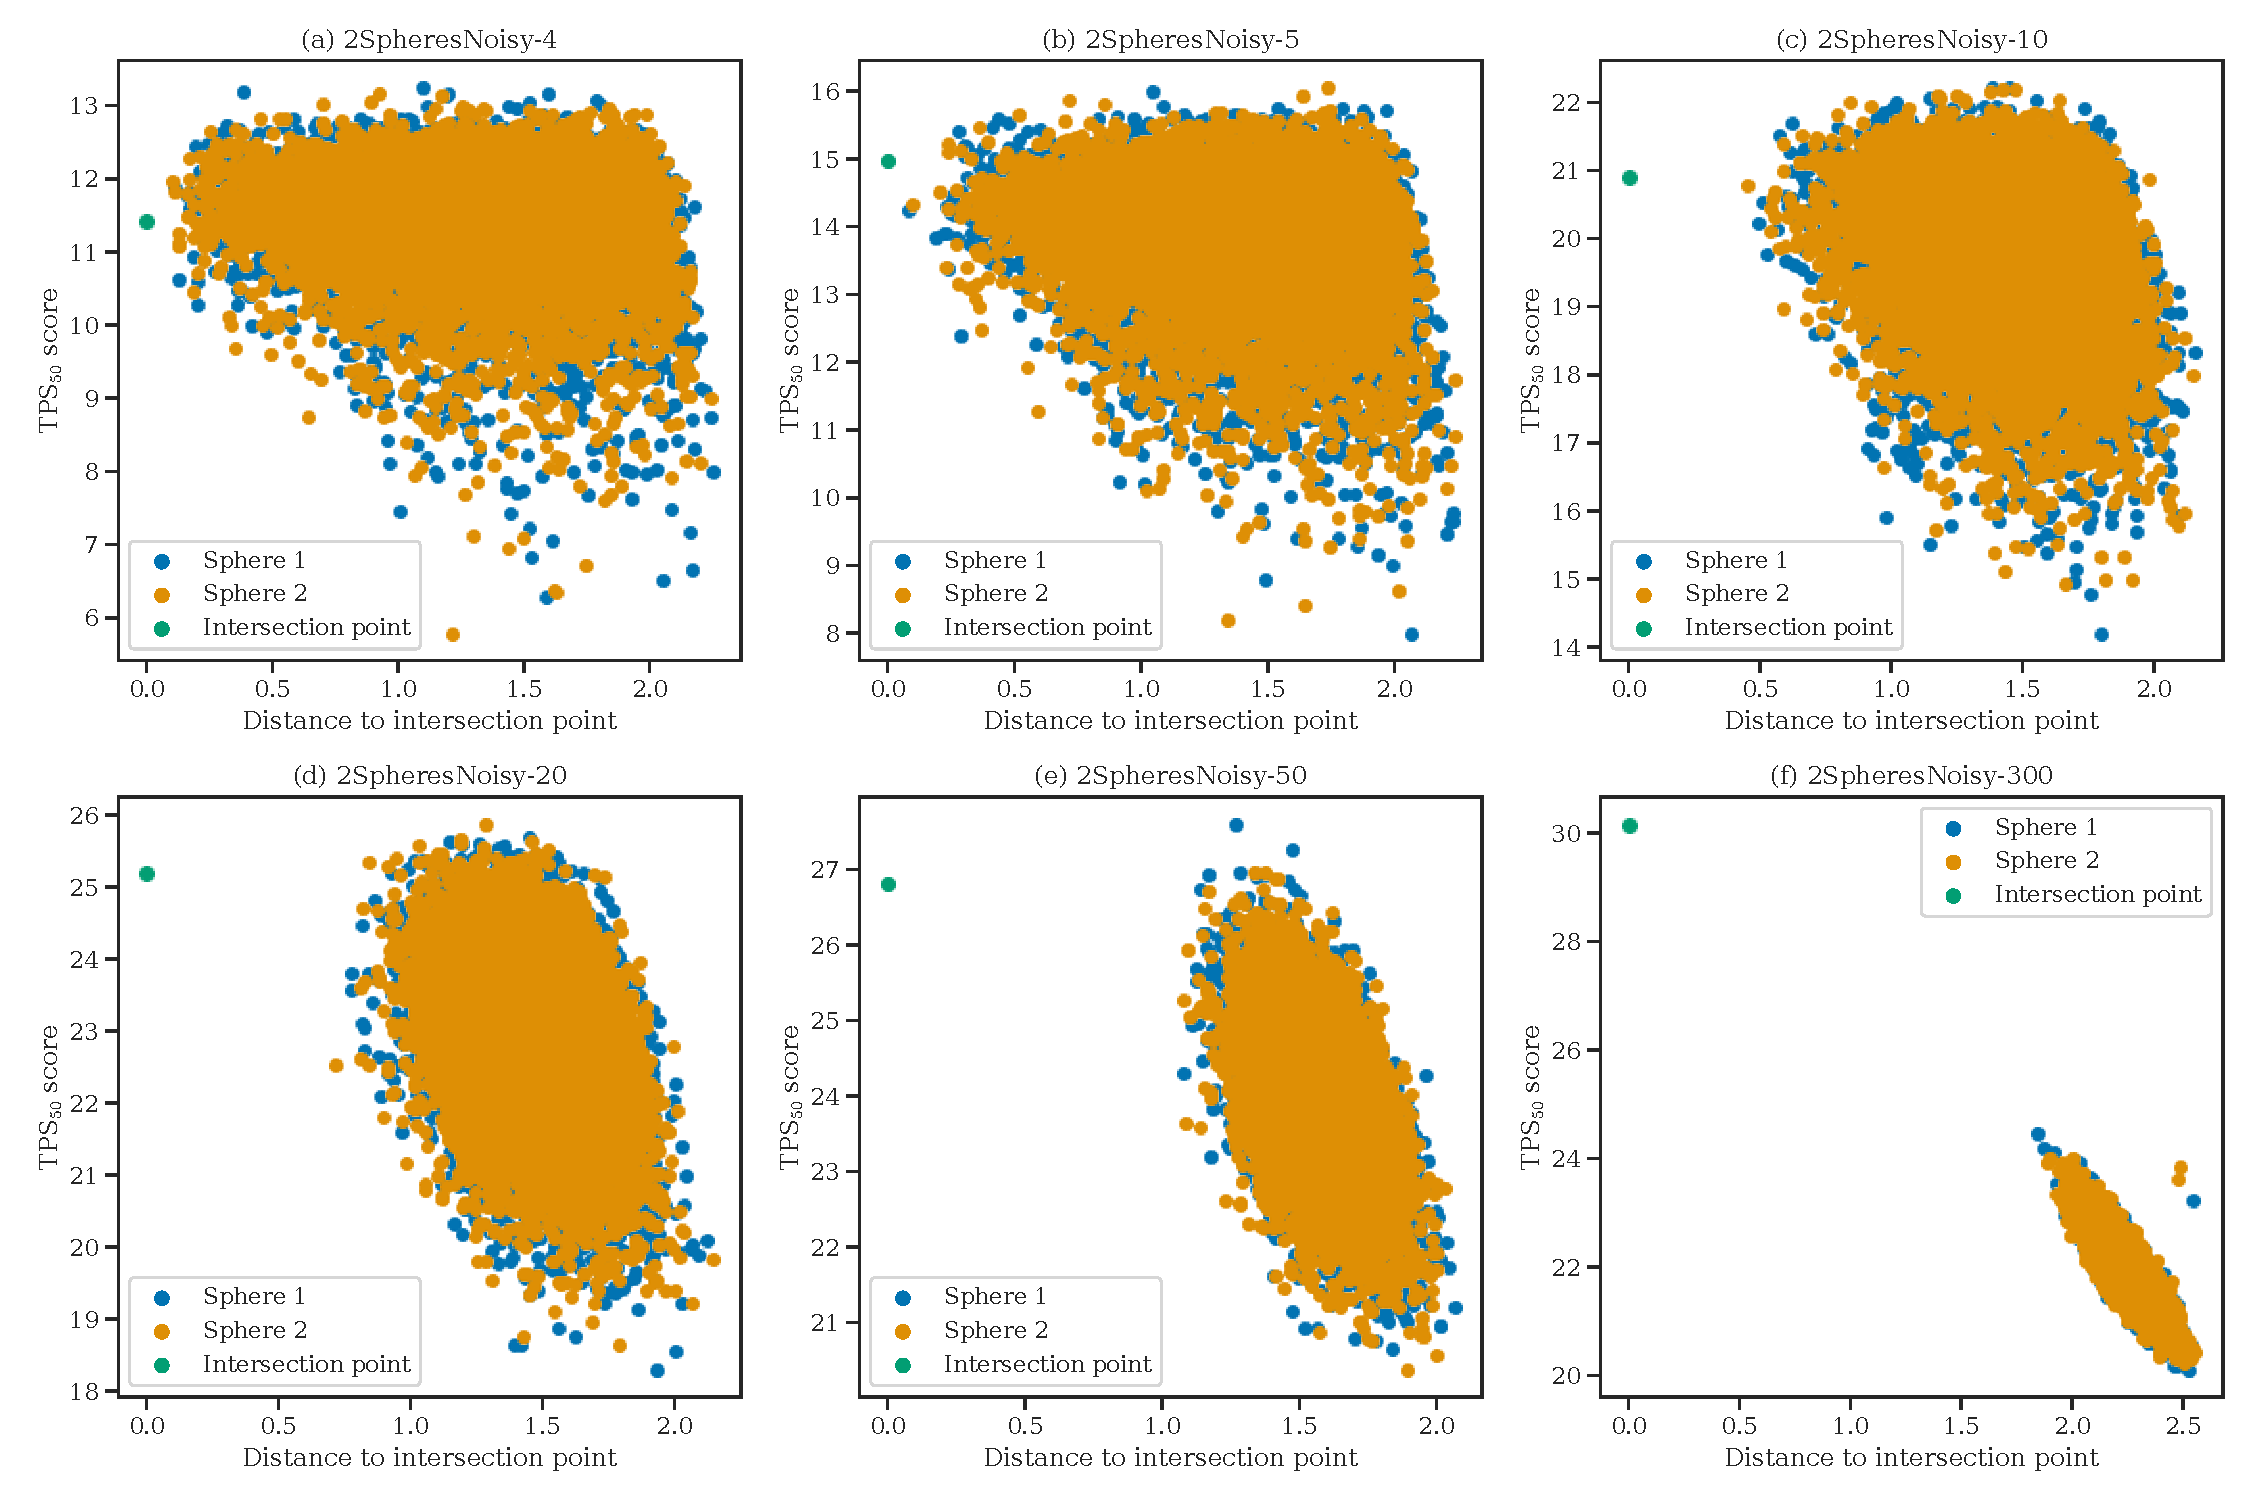
\includegraphics[width=\textwidth]{thesis/figures/two-spheres-noisy-distance-to-int-point-vs-tps-scores.pdf}
    \caption{Distance to intersection point between spheres plotted against $\text{TPS}_{50}$ score for 2SpheresNoisy-$d$, $d \in \enclc{4, 5, 10, 20, 50, 300}$.}
    \label{fig:two-spheres-noisy-distance-to-int-point-vs-tps-scores}
\end{figure}

The measure of topological polysemy will further be used in the supervised polysemy prediction experiments of \cref{sec:analysis-of-embeddings-supervised-polysemy-prediction}, where we create a model for predicting whether or not a word is polysemous. Next, we will look at Geometric Anomaly Detection, and in particular, how it performs when applied to word embeddings.

\subsection{Geometric Anomaly Detection}
\label{sec:analysis-of-embeddings-geometric-anomaly-detection}
In this subsection, we will apply the Geometric Anomaly Detection (GAD) (\cref{sec:geometric-anomaly-detection}) algorithm to the word embeddings from the SGNS-enwiki model. In particular, we will show the relationship between how GAD categorizes word embeddings into groups and whether or not a word is polysemous. Prior to this, we will motivate the use of GAD by visualizing GAD applied to the 3-dimensional \textit{Henneberg surface} data set, as used in the experiments of \cite{stolz2020geometric}. To implement GAD, we used similar packages to the ones used to implement topological polysemy in \cref{sec:analysis-of-embeddings-topological-polysemy}, namely the ScaNN \cite{scann2020} approximate nearest neighbour algorithm, to speed up the nearest-neighbour computation, and \path{ripser} \cite{ctralie2018ripser} Python package, to compute Vietoris–Rips complexes. We also included an option to use Ripser++ \cite{zhang2020ripserplusplus} (Ripser "plus plus") instead of \path{ripser}, a GPU accelerated version of \path{ripser}, but we would that the GPU overhead was too large and it was faster just to use the regular \path{ripser} Python package. 

Next, we apply GAD to the Henneberg surface data set, using the same hyperparameters used by \cite{stolz2020geometric}; we let the inner annulus radius equal 1.5, outer annulus radius equal 2 and the manifold dimension $k$ equal 2. The result is visualized in \cref{fig:gad-henneberg-3d}, and we see how GAD groups data points to the manifold, boundary and singular groups. In the 3-dimensional Henneberg surface data set, there are four 2-dimensional surfaces which intersect, as shown by the plot to the right (b) of \cref{fig:gad-henneberg-3d}, where the GAD algorithm correctly identified them (singular points). In addition to the singular points, the boundary points are also nicely shown in in both plots (a) and (b).
\begin{figure}[H]
    \centering
    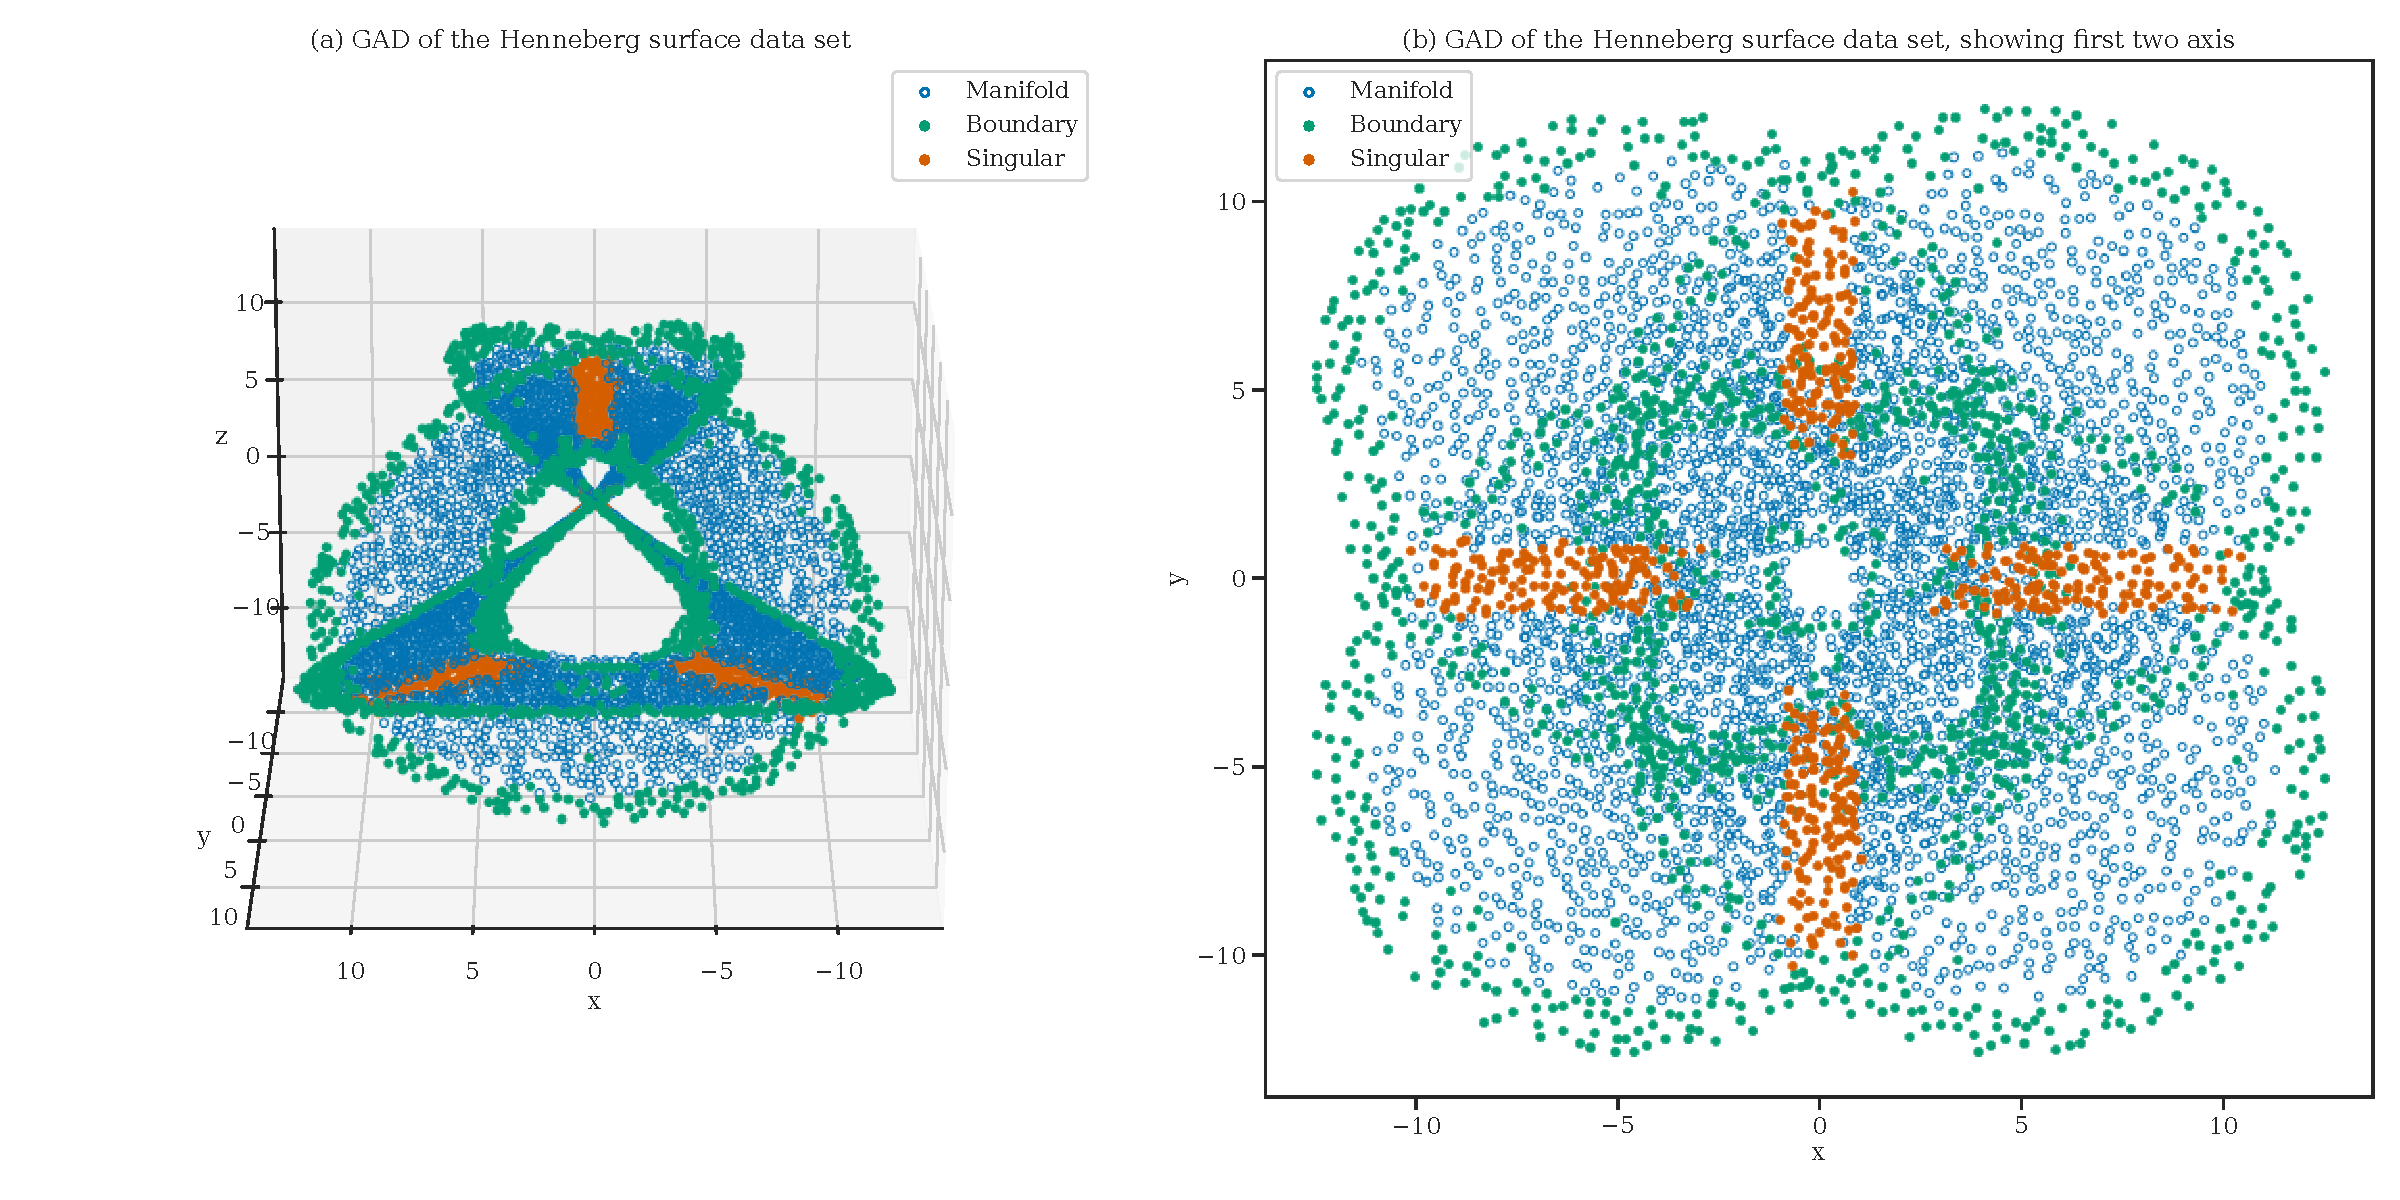
\includegraphics[width=\textwidth]{thesis/figures/gad-henneberg-3d.pdf}
    \caption{2D and 3D projections of the Henneberg surface data set, labeled with the data point groups from the GAD algorithm. This figure is inspired by \cite[Figure 3]{stolz2020geometric}.}
    \label{fig:gad-henneberg-3d}
\end{figure}

Following, we visualize the Henneberg surface data set with the $\text{TPS}_{50}$ score computed for each point. As shown in \cref{fig:gad-henneberg-3d-tps-50}, we see that the measure of topological polysemy fails to identify the singular data points, which we expect to have a relatively high $\text{TPS}_{50}$ score. In particular, the $\text{TPS}_{50}$ score is relatively high for points on the manifold, and lower for the boundary and singular points.
\begin{figure}[H]
    \centering
    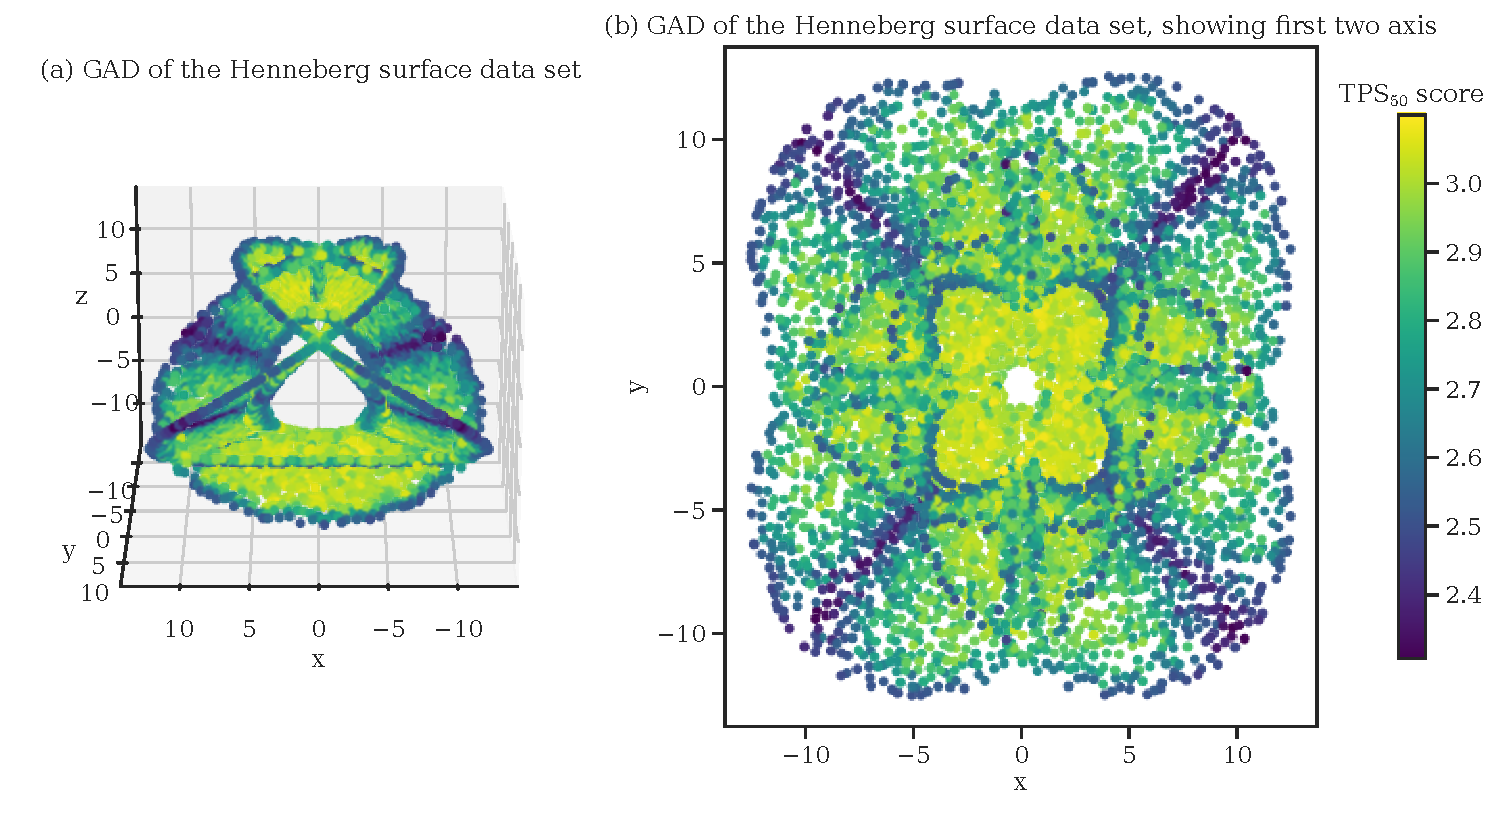
\includegraphics[width=\textwidth]{thesis/figures/gad-henneberg-3d-tps-50.pdf}
    \caption{2D and 3D projections of the Henneberg surface data set, labeled with the $\text{TPS}_{50}$ score for each point.}
    \label{fig:gad-henneberg-3d-tps-50}
\end{figure}

We now apply GAD to the word embeddings from the SGNS-enwiki model. In particular, we will compute GAD of the words which have a WordNet entry, similar to the word embeddings used in the SGNS-enwiki experiments with topological polysemy in \cref{sec:analysis-of-embeddings-topological-polysemy}. Since we do not know a good set of annulus radii parameters to use when computing GAD of the WordNet SGNS-enwiki word embeddings, we will instead default to a $k$-nearest neighbour approach, where we let the inner annulus radius equal to the distance to the $s$ nearest neighbour of each word, and similarly for the outer annulus radius, which we set equal to the distance to the $t$ nearest neighbour of each word. To compute GAD of the WordNet SGNS-enwiki word embeddings, we used the parameters $s=25$ and $t=500$. The number of words in each GAD group is shown in \cref{table:number-of-words-gad-polysemous-sgns-enwiki-wordnet}. From \cref{table:number-of-words-gad-polysemous-sgns-enwiki-wordnet}, we see that the number of polysemous WordNet words that fall into the singular group is particularly low; only 344 of 48880. In addition to this, we see that the number of words being categorized as "boundary" words is high. These two observations suggest that our inner and outer annulus radius, as well as the manifold dimension $k$, were not set correctly for we are working with. Keep in mind that the intrinsic dimensionality of the word embeddings are most likely higher than $k=2$, but due to the computational cost of setting $k > 2$ (due to Vietoris–Rips complex creation), we will not set $k$ greater than 2 in this thesis.
\begin{table}[H]
    \centering
    \begin{tabular}{@{}lcccl@{}}
    \toprule
    \multicolumn{1}{c}{}       & \multicolumn{3}{c}{GAD group}  & \multicolumn{1}{l}{} \\ \cmidrule(lr){2-4}
    \multicolumn{1}{c}{}       & Manifold & Boundary & Singular & \textit{Sum}                  \\ \midrule
    \trcolor Number of monosemous words            & 4 640     & 86 731    & 4 161     & 95 532                \\
    Number of polysemous words & 634      & 47 902    & 344      & 48 880                \\ \midrule
    \trcolor \textit{Sum}                        & 5 274     & 134 633   & 4 505     & 144 412 \\ \bottomrule
    \end{tabular}
    \caption{Number of mono- and polysemous words in each GAD group, when applied to the WordNet SGNS-enwiki word embeddings.}
    \label{table:number-of-words-gad-polysemous-sgns-enwiki-wordnet}
\end{table}

Furthermore, we visualize the result using a 2-dimensional UMAP embedding of the 10000 most common words of the the WordNet SGNS-enwiki word embeddings, labeled using the GAD groups, as seen in \cref{fig:gad-umap-2d-10k-most-common-wordnet-enwiki-words}. From \cref{fig:gad-umap-2d-10k-most-common-wordnet-enwiki-words}, we see that only a single word has been categorized as singular (the word "branch"), some words are categorized as manifold and the rest are categorized as boundary. The fact that most words are categorized as boundary further strengthens our hypothesis that the hyperparameters used to compute GAD are not correct. We also observe that \cref{fig:gad-umap-2d-10k-most-common-wordnet-enwiki-words} differs a whole lot from GAD applied to the Henneberg surface data set (\cref{fig:gad-henneberg-3d}), which could indicate bad hyperparameterization.
\begin{figure}[H]
    \centering
    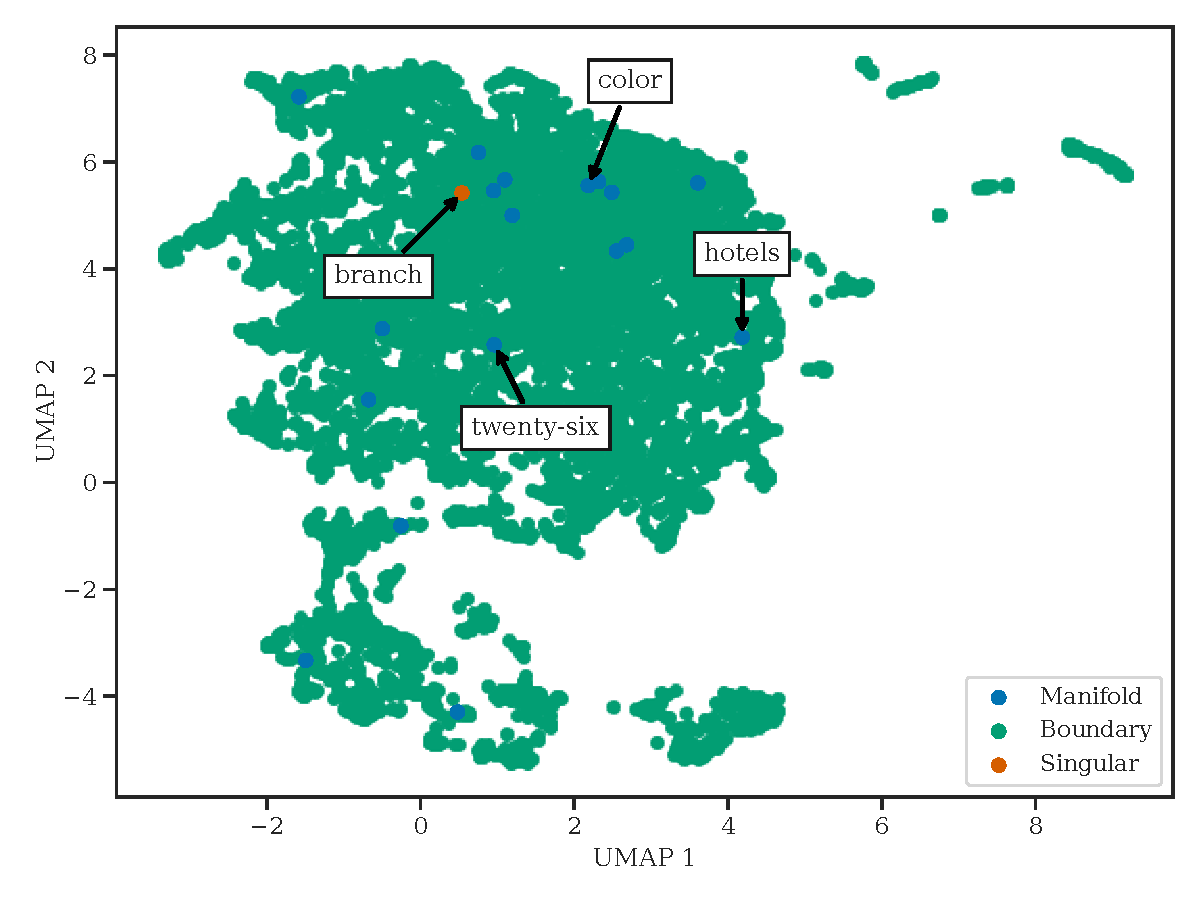
\includegraphics[width=0.8\textwidth]{thesis/figures/gad-umap-2d-10k-most-common-wordnet-enwiki-words.pdf}
    \caption{2-dimensional UMAP embedding of the 10000 most common words from the WordNet SGNS-enwiki word embeddings. The words are labeled using its GAD group.}
    \label{fig:gad-umap-2d-10k-most-common-wordnet-enwiki-words}
\end{figure}

We will investigate the effect of using different sets of hyperparameters when computing GAD of word embeddings in \cref{sec:analysis-of-embeddings-supervised-polysemy-prediction}, where we will create supervised models for predicting whether or not a word is polysemous. Next, we will investigate algorithms for estimating the intrinsic dimensionality of word embeddings, and how it correlates with the actual number of word meanings.

\subsection{Intrinsic dimension estimation}
\label{sec:analysis-of-embeddings-intrinsic-dimension-estimation}
In this subsection, we will look at intrinsic dimension (ID) estimation algorithms (\cref{sec:intrinsic-dimension-estimation}) and apply them to word embeddings. In particular, we will apply ID estimation algorithms to the WordNet SGNS-enwiki word embeddings, used in experiments in \cref{sec:analysis-of-embeddings-topological-polysemy} and \cref{sec:analysis-of-embeddings-geometric-anomaly-detection}. We show the relationship between the estimated ID and the number of WordNet word meanings. To demonstrate the relationship between estimated ID and number of WordNet word meanings, we will use the LPCA (\cref{sec:id-estimation-lpca}), TWO-NN (\cref{sec:id-estimation-twonn}) and TLE (\cref{sec:id-estimation-tle}) algorithms. For each algorithm, we compute the estimated local intrinsic dimension by using the 200 nearest neighbour of each word. We plot the estimated IDs versus the number of WordNet word meanings in \cref{fig:intrinsic-dimension-estimation-vs-wordnet-synsets}, and we observe a similar behaviour shown in \cref{fig:tps-n-correlation-sgns-enwiki} and \cref{fig:tps-n-correlation-sgns-semeval}, namely that we see a clear trend when plotted against the number of WordNet word meanings. We also see that, the different ID estimation algorithms yield different results; LPCA estimates ID up to 120, while TWO-NN and TLE estimates ID up to 50 and 60. This result suggest that, we can not simply rely on a single estimate of the ID, it could be useful to use multiple ID estimates, as they are measured differently (see \cref{sec:intrinsic-dimension-estimation} for more details).
\begin{figure}[H]
    \centering
    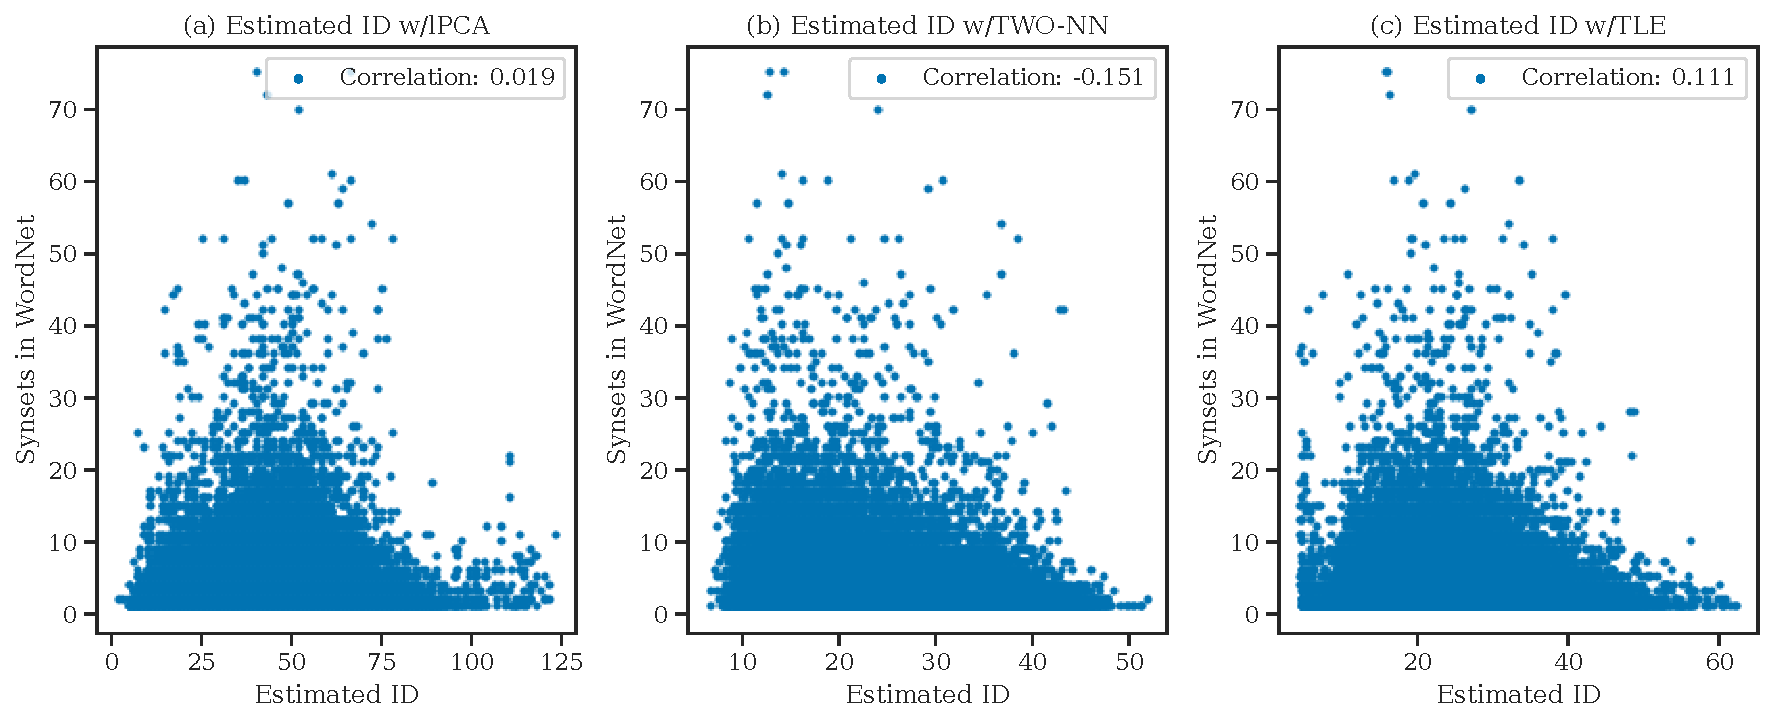
\includegraphics[width=\textwidth]{thesis/figures/intrinsic-dimension-estimation-vs-wordnet-synsets.pdf}
    \caption{Estimated IDs plotted against number of word meanings, using LPCA, TWO-NN and TLE ID estimation algorithms.}
    \label{fig:intrinsic-dimension-estimation-vs-wordnet-synsets}
\end{figure}

We have now shown the relationship between estimated ID and number of word meanings. In the next section, we will create supervised models for predicting whether or not a word is polysemous. We will use multiple sets of hyperparameters and all ID estimation algorithms specified in \cref{sec:intrinsic-dimension-estimation}, as well the topological polysemy (\cref{sec:analysis-of-embeddings-topological-polysemy}) and Geometric Anomaly Detection (\cref{sec:analysis-of-embeddings-geometric-anomaly-detection}) algorithms.

\subsection{Supervised polysemy prediction}
\label{sec:analysis-of-embeddings-supervised-polysemy-prediction}
In this subsection, we propose two supervised models to predict the number of word meanings. As we have seen in the previous subsections (\cref{sec:analysis-of-embeddings-topological-polysemy}, \cref{sec:analysis-of-embeddings-geometric-anomaly-detection} and \cref{sec:analysis-of-embeddings-intrinsic-dimension-estimation}), the number of word meanings seem to be more or less correlated with topological polysemy, Geometric Anomaly Detection (GAD) and intrinsic dimension (ID) estimation. For this reason, we propose two supervised model using lasso regression (\cref{sec:lasso-regression}) and logistic regression (\cref{sec:logistic-regression}), incorporating the results from topological polysemy, GAD and ID estimation. We chose to use lasso regression, because it has feature importance packed in the model. The feature importance part is important for us, because we would like to try multiple configurations of hyperparameters for each algorithm used to create the training data. The logistic regression model is trained using $\ell_1$-penalty, which allows the model to perform feature importance as well. The lasso regression model tries to predict the number of word meanings, while the logistic regression model performs binary prediction of whether or not a word is polysemous. We also attempted to create a multi-class (e.g. 1 meaning, 2 meanings, etc.) model using multinomial logistic regression, but it became apparent that the problem was too hard and we decided not to follow up with those experiments. Furthermore, we denote the lasso regression model as \textit{WME-enwiki} (short for \textbf{W}ord \textbf{M}eaning \textbf{E}stimation-enwiki) and the logistic regression model as \textit{BWME-enwiki} (short for \textbf{B}inary \textbf{W}ord \textbf{M}eaning \textbf{E}stimation-enwiki). Next, we will describe the creation of training data used for both supervised models, before going into detail of the training and evaluation process.

To create the training data used in the WME- and BWME-enwiki models, we used the word embeddings from the SGNS-enwiki model. In particular, we used the word embeddings that have a WordNet entry, resulting in 144 412 words. We denote these word embeddings as the WordNet SGNS-enwiki word embeddings. The number of word meanings (i.e. number of WordNet symsets) are used as labels $y$ for the WME-enwiki model, while the BWME-enwiki model have binary labels, $y=0$ if the word have exactly one word meaning, and $y=1$ if the word has two or more meanings.

To create the features of the training data, we first compute topological polysemy $\text{TPS}_n(w)$ of the WordNet SGNS-enwiki word embeddings. We compute $\text{TPS}_n(w)$ at for varying $n=10, 20, 30, \ldots, 250$ (step size of 10, leading to 25 values of $n$) and use them as features in the data. In addition to this, we compute the maximum, average and standard deviation of the birth values of the zero-degree persistence diagram computed by $\text{TPS}_n(w)$, leading to 3 additional features for each $\text{TPS}_n(w)$. In total, we get 25 (values of $n$) $\times$ 4 = 100 features from topological polysemy.

Following, we compute GAD of the WordNet SGNS-enwiki word embeddings. To compute GAD, we use the $k$-nearest neighbour version, similar to the experiments of \cref{sec:analysis-of-embeddings-geometric-anomaly-detection}; we let the inner annulus radius equal the distance to the $s$-nearest neighbour and the outer annulus radius equal the distance to the $t$-nearest neighbour. By using the $k$-nearest neighbour version of GAD, we are also in more control of how long it takes to compute GAD (setting the radius manually can lead to big and difficult computations of the Vietoris–Rips complex, since some areas are more dense than others). The different choices of $s$ and $t$ are shown in \cref{table:supervised-polysemy-prediction-gad-configurations}, and leads to 23 different configurations of the inner and outer annulus $k$-nearest neighbours. We let the manifold dimension $k$ equal 2 for all words, even though the local intrinsic dimension for each word is likely higher than 2. This was done to make the GAD computation feasible within the computational resources at hand; we will revisit the manifold dimension choice when discussing future work in \cref{chap:conclusion-and-future-work}. For each configuration used in GAD, we create one feature for each GAD group (manifold, boundary and singular) by using one-hot encodings; e.g. if a word is categorized as manifold, then its value is equal to 1 and the rest are set to zero. In other words, we are left with 23 (configurations) $\times$ 3 (GAD groups) = 69 features from GAD. We also attempted to vectorize the persistence diagrams created by GAD using persistence images (\cref{sec:persistence-image}), but it quickly led to far too many features as we used each pixel in the images as a separate feature, and we were unable to train the WME- and BWME-enwiki models efficiently. We will revisit the use of persistence images when discussing future work in \cref{chap:conclusion-and-future-work}.
\begin{table}[H]
    \centering
    \begin{tabular}{@{}cc@{}}
    \toprule
    \multicolumn{1}{l}{Inner annulus, $s$-nearest neighbour} & \multicolumn{1}{l}{Outer annulus, $t$-nearest neighbour} \\
    \midrule
    \trcolor 25 & 250 \\
    25 & 500 \\
    \trcolor 25 & 750 \\
    25 & 1000 \\
    \midrule
    \trcolor 50 & 250 \\
    50 & 500 \\
    \trcolor 50 & 750 \\
    50 & 1000 \\
    \midrule
    \trcolor 100 & 1000 \\
    100 & 1250 \\
    \trcolor 100 & 1500 \\
    100 & 1750 \\
    \trcolor 100 & 2000 \\
    \midrule
    150 & 1000 \\
    \trcolor 150 & 1250 \\
    150 & 1500 \\
    \trcolor 150 & 1750 \\
    150 & 2000 \\
    \midrule
    \trcolor 200 & 1000 \\
    200 & 1250 \\
    \trcolor 200 & 1500 \\
    200 & 1750 \\
    \trcolor 200 & 2000 \\
    \bottomrule
    \end{tabular}
    \caption{Configurations of $s$ (inner annulus nearest neighbour) and $t$ (outer annulus nearest neighbour) for computing GAD of the WordNet SGNS-enwiki word embeddings.}
    \label{table:supervised-polysemy-prediction-gad-configurations}
\end{table}

Furthermore, we estimate the local ID of all WordNet SGNS-enwiki word embeddings, using the ID estimator algorithms in \cref{sec:intrinsic-dimension-estimation}. More precisely, we used the LPCA (\cref{sec:id-estimation-lpca}), KNN (\cref{sec:id-estimation-knn}), TWO-NN (\cref{sec:id-estimation-twonn}), MLE (\cref{sec:id-estimation-mle}) and TLE (\cref{sec:id-estimation-tle}) algorithms. For each of the algorithms, we formed a $k$-nearest neighbourhood around each word and estimated the local ID of the neighbourhood. We used the following values for $k$: 25, 50, 100, 150 and 200. The estimated local ID of each word is used as a feature in the training data, leading to 5 (algorithms) $\times$ 5 (hyperparameter sets) = 25 features from ID estimation. We used the \path{scikit-dimension} Python package \cite{scikitdimension2020} to estimate the local IDs.

In total, the training data has 100 (from topological polysemy) + 69 (from GAD) + 25 (from ID estimation) = 194 features. Following, we split the training data into three new distinct data sets (\cref{sec:train-val-test-splits}): training-, test- and SemEval test data sets. The new training data set consist of 95\% random words of the original training data set, where the 100 SemEval-2010 Task 14 target words (\cref{sec:analysis-of-embeddings-topological-polysemy}) are excluded. The test data set consist consist of 5\% random words of the original training data set, where the 100 SemEval-2010 Task 14 target words are excluded. The test data set will be used to evaluate the performance of the WME- and BWME-enwiki models. The SemEval test data set consist of the 100 SemEval-2010 Task 14 target words, and will be used to evaluate the performance using the WME-enwiki model, as well. We would like to emphasize that the training and test data sets do not have overlapping words, as we do not want to be training on words from the test data sets. The training data set consists of 137 098 words, test data set consists of 7 216 words and the SemEval test data set consist of 98 words (as 2 of the words are out of the SGNS-enwiki vocabulary). For each data set, we transform the features by removing the mean and scaling to unit variance, as we do not want the WME- and BWME-enwiki models to be affected by different means and variances across the features. For the SemEval test data set, we use the SemEval gold standard to be the number of word meanings, while for the training and test data set we use the number of WordNet synsets as the number of word meanings.

Following, we trained the WME- and BWME-enwiki models using $k$-fold cross validation (\cref{sec:cross-validation}). We found $k=20$ to work well with out data, meaning that we use 6 855 words random validation for each fold in the cross-validation. For the WME-enwiki model, we cross-validated over 10000 values for $\lambda$, starting from $\lambda=0.0000001$ to $\lambda=0.01$. We found the most optimal value for the WME-enwiki model to be $\lambda=0.0000291$. For the BWME-enwiki model, we cross-validated over 10000 values for $\lambda$, starting from $\lambda=0.00001$ to $\lambda=0.01$. We found the most optimal value for the BWME-enwiki model to be $\lambda=0.000692$. To perform the cross-validation we used the \path{LassoCV} and \path{LogisticRegressionCV} classes from \path{scikit-learn} for the WME- and BWME-enwiki models, respectively. We used the sensitivity metric (\cref{sec:sensitivity}) to score the folds from the BWME-enwiki cross validation, as the sensitivity is intuitively the ability of the model to find all the polysemous words. For the WME-enwiki model, we used the default scoring of the \path{LassoCV} class. Results from training the WME-enwiki model is shown in \cref{fig:wme-enwiki-correlation-result}, where we see a weak correlation between the predicted number of word meanings and the number of WordNet synsets for both the training (a) and test data sets (b). The last plot (c) shows that the model is unable to predict the number of word meanings for the SemEval data set, which is not surprising, since we have trained using the number of WordNet synsets. We note, however, that we see clear trends in all plots.
\begin{figure}[H]
    \centering
    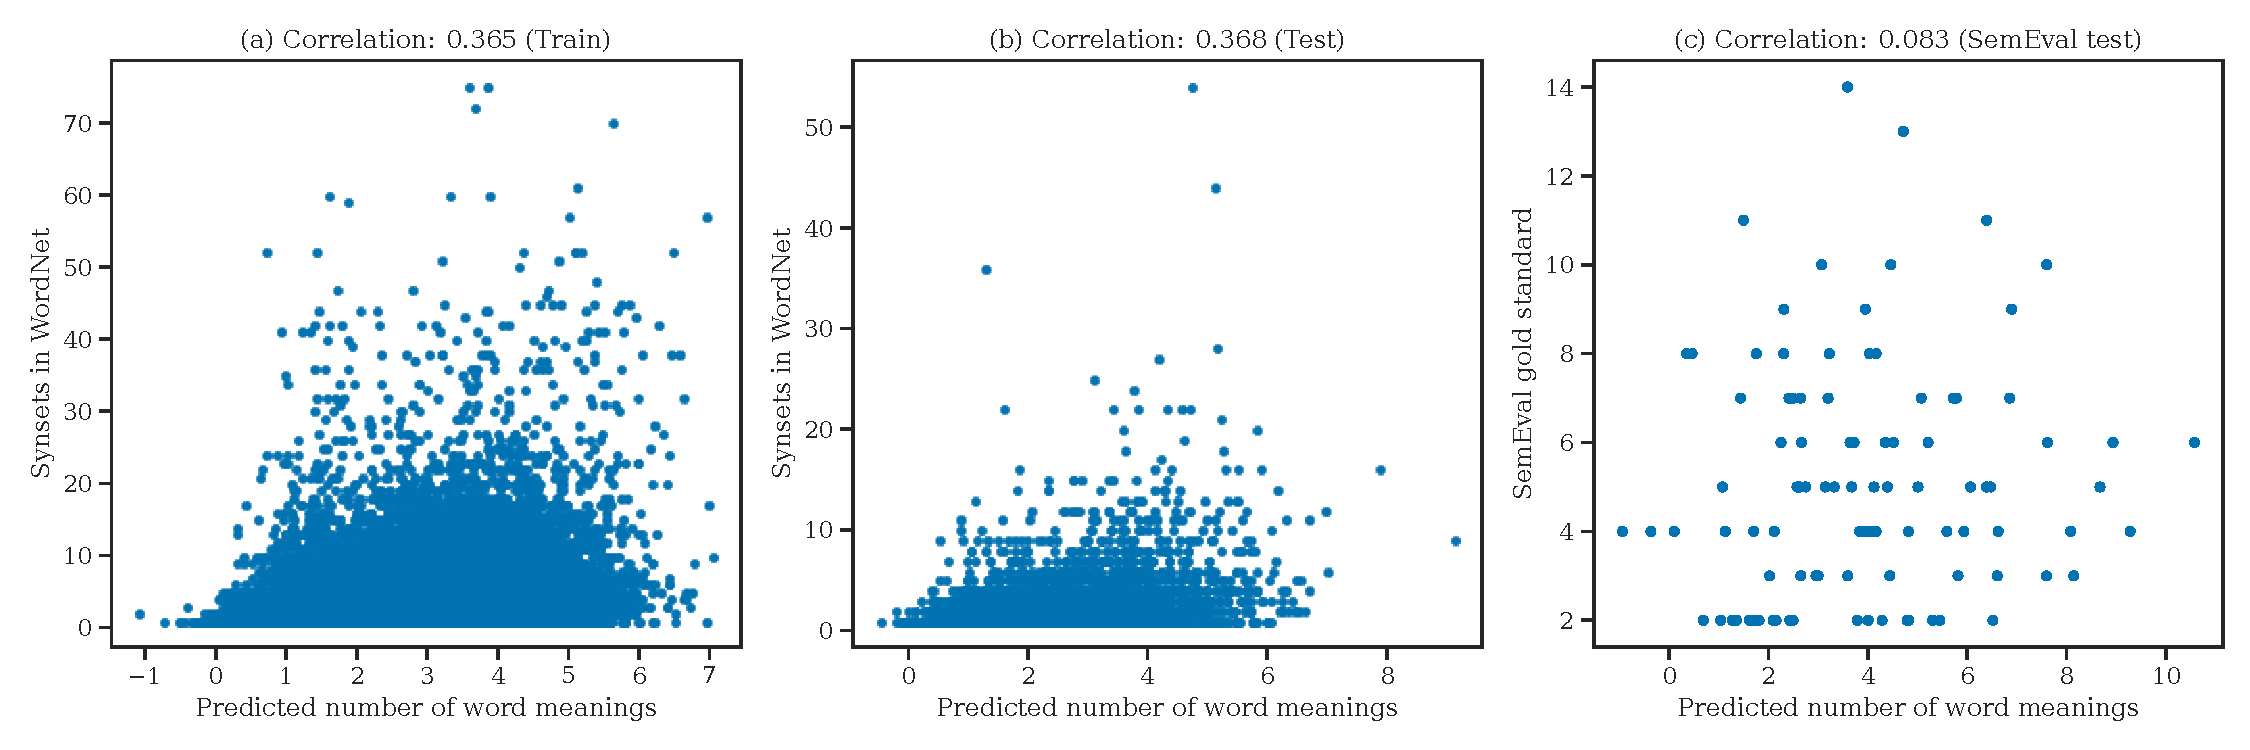
\includegraphics[width=\textwidth]{thesis/figures/wme-enwiki-correlation-result.pdf}
    \caption{Predicted number of word meanings plotted against number of WordNet synsets and SemEval gold standard, using the WME-enwiki model.}
    \label{fig:wme-enwiki-correlation-result}
\end{figure}

By looking at the values of the coefficients of the WME-enwiki model, we see how the model prioritizes certain features over others. We visualize the top 10 most important features in \cref{fig:wme-enwiki-feature-importances}. From \cref{fig:wme-enwiki-feature-importances} we see that the features from topological polysemy for high values of $n$ are the most relevant for the model. The MLE and TLE intrinsic dimension estimators are also relatively relevant for high values of the $k$-nearest neighbour. The features from GAD are not in the top 10 most important features.
\begin{figure}[H]
    \centering
    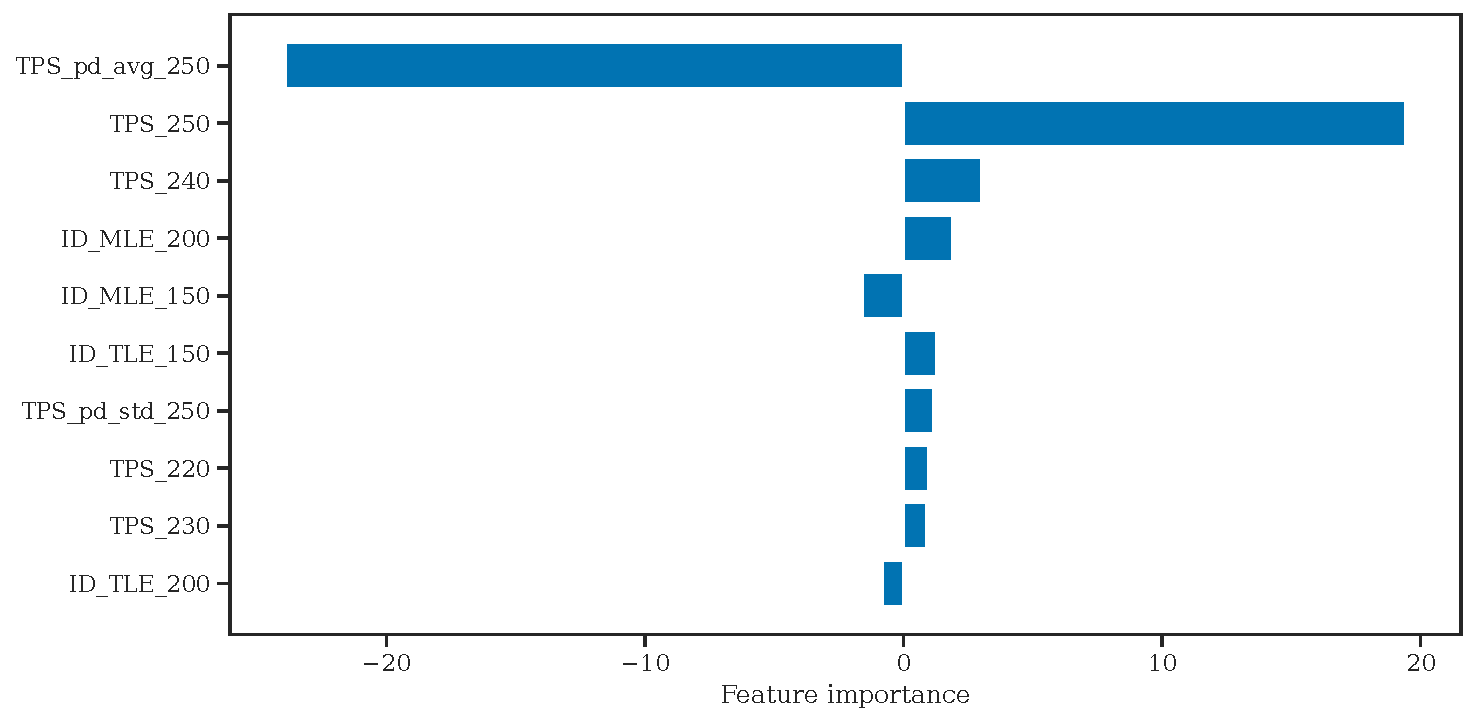
\includegraphics[width=\textwidth]{thesis/figures/wme-enwiki-top-10-feature-importances.pdf}
    \caption{Feature importances for the top 10 most important features of the WME-enwiki model.}
    \label{fig:wme-enwiki-feature-importances}
\end{figure}

To investigate the feature importances for the TPS, GAD and ID estimator features, we visualize its top 10 most important features in \cref{fig:wme-enwiki-feature-importances-tps-gad-estimated-ids}. From \cref{fig:wme-enwiki-feature-importances-tps-gad-estimated-ids}, we see that the $\text{TPS}_{250}$ features are especially relevant, show in (a). The GAD features from (b) show that whether or not a word is classified as a boundary or singular word is important, while whether or not a word is on the manifold is not as relevant. Lastly, we see that the MLE and TLE ID estimator methods yield important features for various values of $n$. It should be noted, that the feature importance shown in (a) and (c) are more important than the features shown in (b), as noted by the x-axis scales.
\begin{figure}[H]
    \centering
    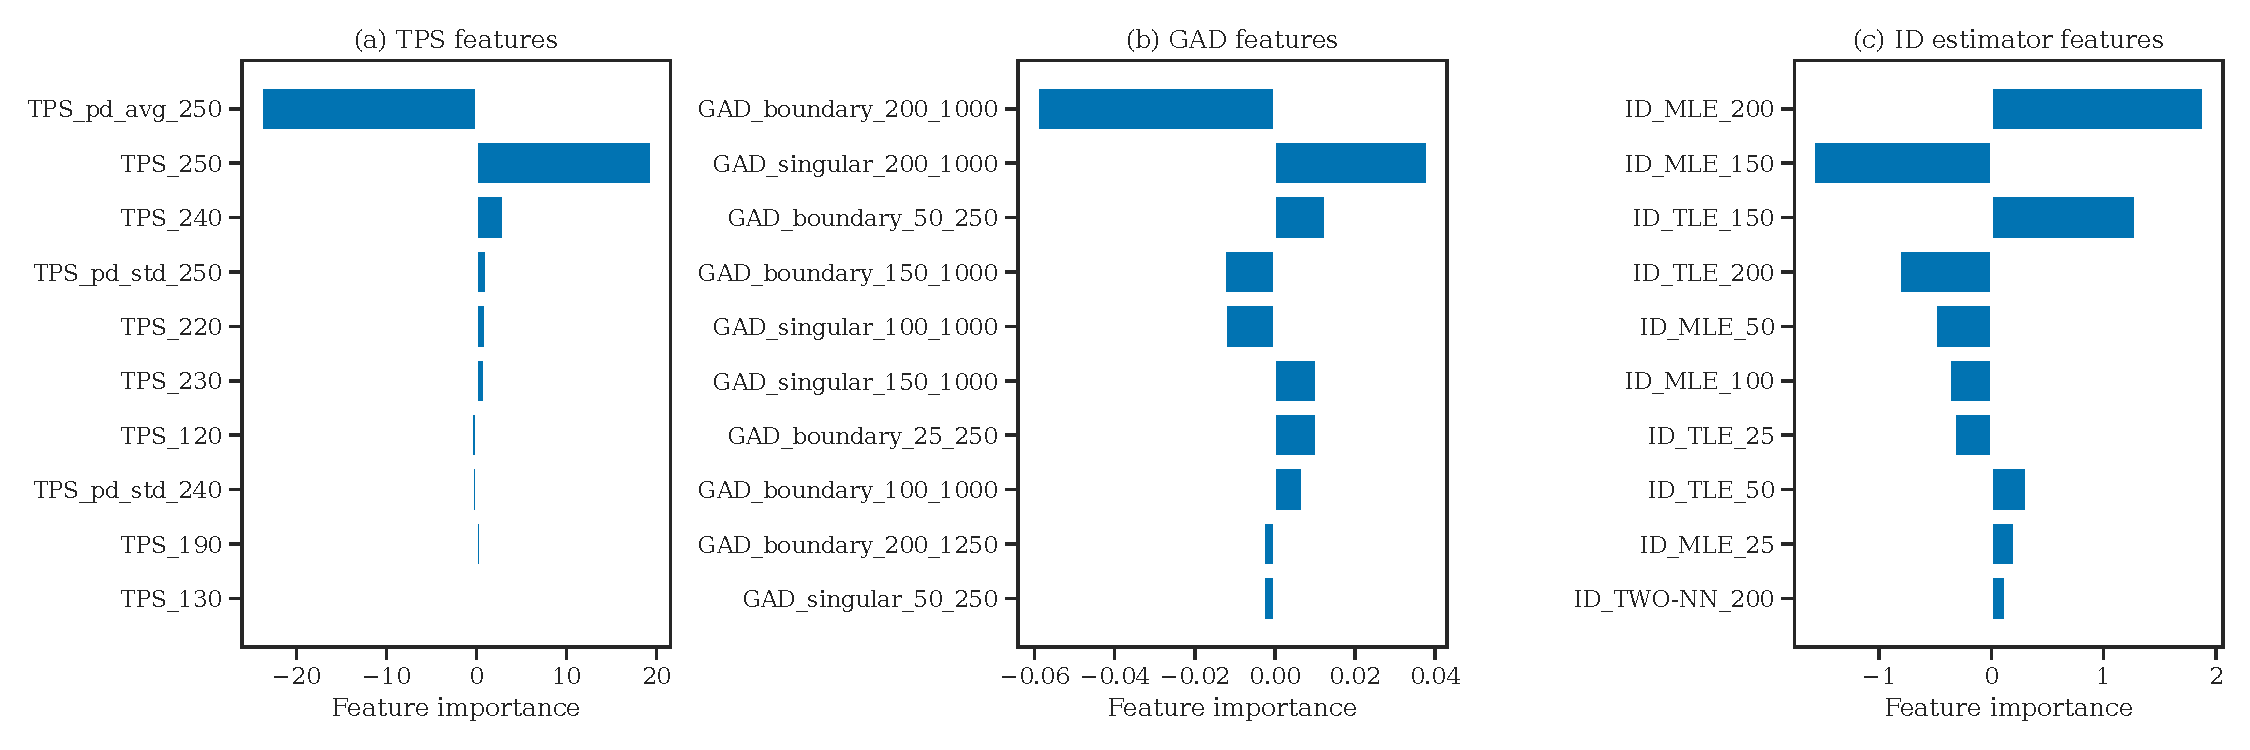
\includegraphics[width=\textwidth]{thesis/figures/wme-enwiki-top-10-feature-importances-tps-gad-estimated-ids.pdf}
    \caption{Feature importance of the top 10 TPS, GAD and ID estimator features, using the WME-enwiki model.}
    \label{fig:wme-enwiki-feature-importances-tps-gad-estimated-ids}
\end{figure}

Some of the features from the WME-enwiki model were also set to zero, meaning that they are not used in the model. In particular, 48 of 194 features were set to zero, and most of them were various configurations of GAD which did not yield any interesting result (e.g. all words classified as boundary words). We have now looked at the result from training of the WME-enwiki model, and in particular, looked at its performance when predicting the number of word meanings and which features were important to the model. Next, we will look at the results from the training of the BWME-enwiki model. Results from training the BWME-enwiki model is shown in \cref{fig:bwme-enwiki-confusion-matrices}, where we see the result of predicting number of word meanings on the training (a) and test (b) data sets using confusion matrices (\cref{sec:confusion-matrix}). From \cref{fig:bwme-enwiki-confusion-matrices}, we get a sensitivity of 0.393 on the train data sets (a), meaning that the model is able to identify 39.3\% of the polysemous words. The test sensitivity (b) shows that the model is able to identify 39.4\% of all the unseen polysemous words. These results indicate that the model is unable to efficiently predict whether or not a word is polysemous, as we ideally would like the sensitivity on both the training and test sets to be at least 0.5 (or 50\%).
\begin{figure}[H]
    \centering
    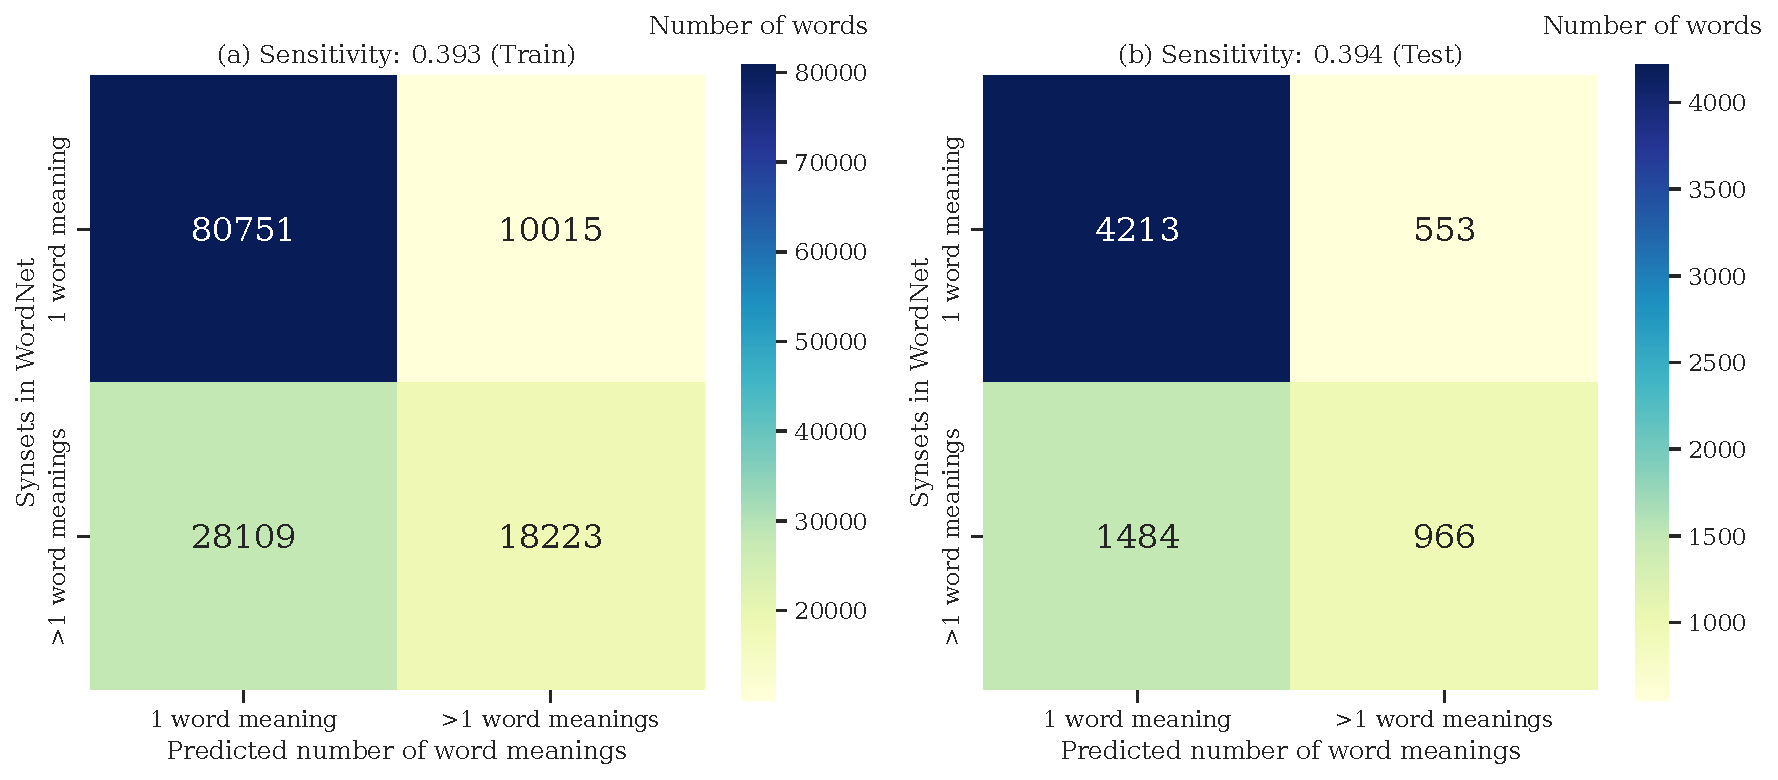
\includegraphics[width=\textwidth]{thesis/figures/bwme-enwiki-confusion-matrices.pdf}
    \caption{Confusion matrices for predicting the number of word meanings, using the BWME-enwiki model. The first confusion matrix (a) shows the result on the training data set, while the second confusion matrix (b) shows the result on the test data set.}
    \label{fig:bwme-enwiki-confusion-matrices}
\end{figure}

To deepen our understanding of which words the BWME-enwiki model has a harder time with, we look at the misclassified polysemous test words. Of the 1484 words the BWME-enwiki model predicted to be monosemous, we report the top 10 most common misclassified test words, namely the following words: "time", "age", "returned", "italian", "chicago", "gold", "tower", "jones", "unable" and "opposition". From these words, we do not see any particular pattern. Furthermore, we visualize the misclassified polysemous test words in \cref{fig:bwme-enwiki-umap-misclassified-polysemous-words}, where we see a 2-dimensional UMAP embedding of the words from the test data set, emphasizing the misclassified polysemous words. In \cref{fig:bwme-enwiki-umap-misclassified-polysemous-words}, we do not see any particular pattern either.
\begin{figure}[H]
    \centering
    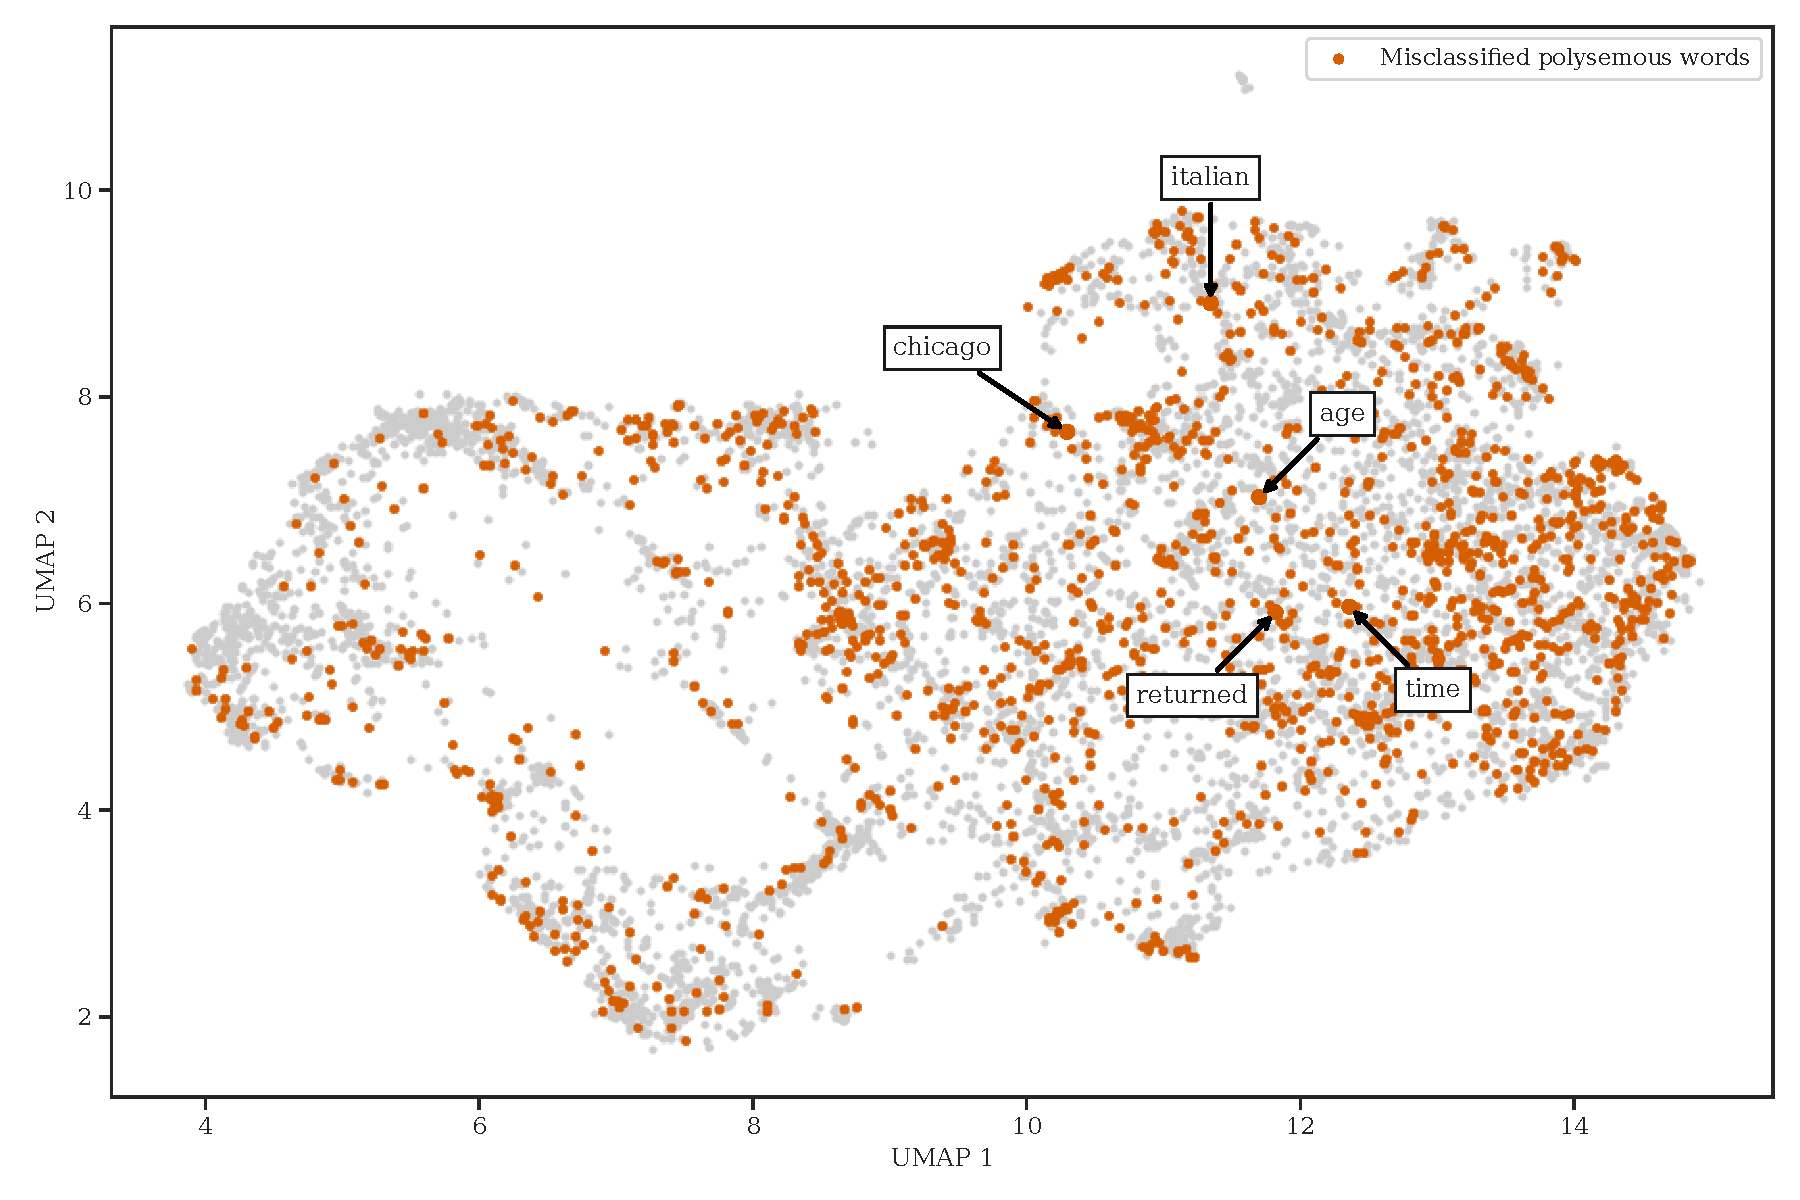
\includegraphics[width=\textwidth]{thesis/figures/bwme-enwiki-umap-misclassified-polysemous-words.pdf}
    \caption{2-dimensional UMAP embedding of the test data set evaluated on the BWME-enwiki model, emphasizing the misclassified polysemous words.}
    \label{fig:bwme-enwiki-umap-misclassified-polysemous-words}
\end{figure}

Next, we will investigate the feature importance in the BWME-enwiki model, by looking at the coefficient values. The feature importance of the BWME-enwiki model is shown in \cref{fig:bwme-enwiki-feature-importances}, where we can see the top 10 most important features. From \cref{fig:bwme-enwiki-feature-importances}, we see a similar pattern to the top 10 features importances from the WME-enwiki model, namely that the TPS features (for varying $n$) are most important, followed by the features from the ID estimator models.
\begin{figure}[H]
    \centering
    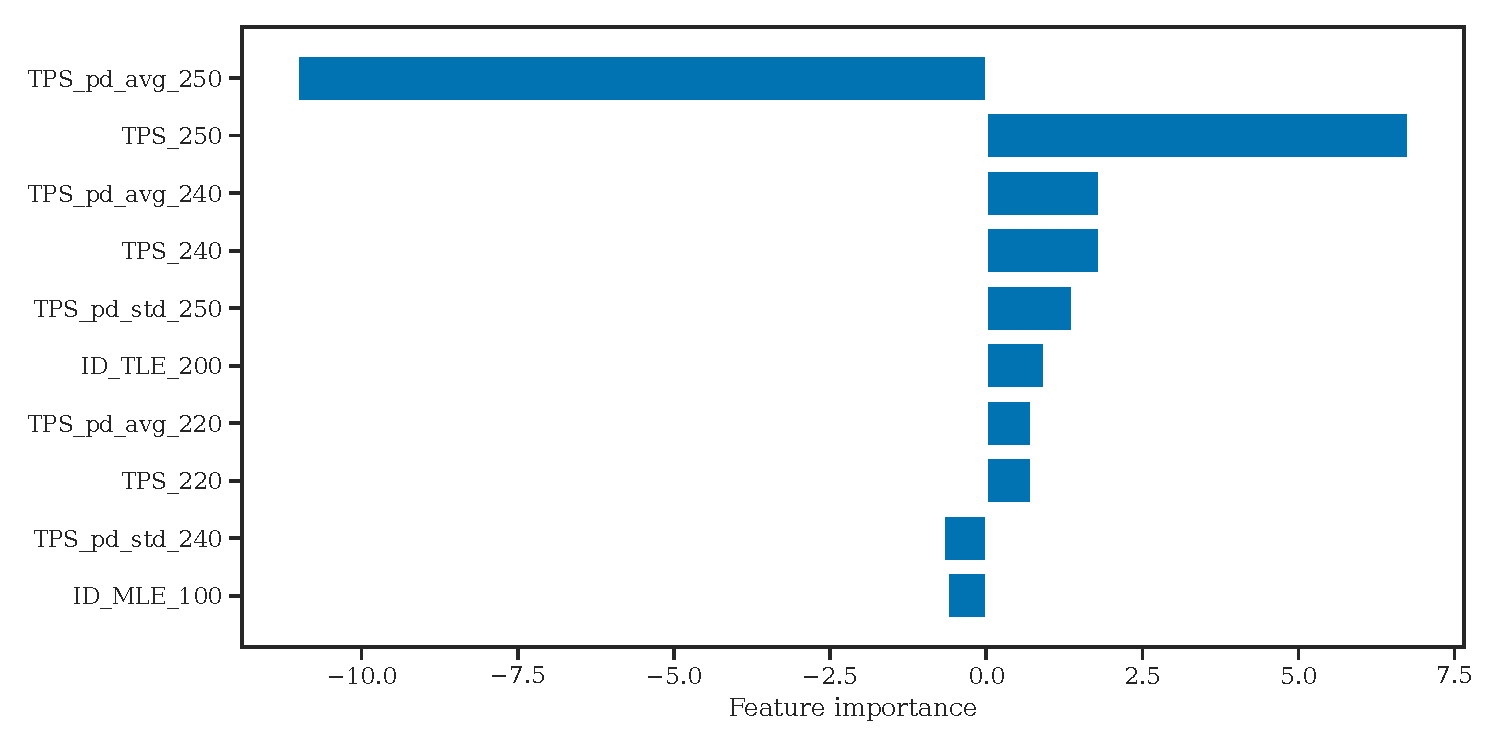
\includegraphics[width=\textwidth]{thesis/figures/bwme-enwiki-top-10-feature-importances.pdf}
    \caption{Feature importances for the top 10 most important features of the BWME-enwiki model.}
    \label{fig:bwme-enwiki-feature-importances}
\end{figure}

Furthermore, we look at the top 10 feature importances for the TPS, GAD and ID estimator features separately, as shown in \cref{fig:bwme-enwiki-feature-importances-tps-gad-estimated-ids}. From \cref{fig:bwme-enwiki-feature-importances-tps-gad-estimated-ids}, we see that the TPS features in plot (a) illustrate that high values of $n$ are generally more important than lower values. The GAD features (b) show a different situation to the top 10 features importances for GAD using the WME-enwiki model; whether or not a point is categorized as singular is important for predicting whether or not a word is polysemous, and the rest of the GAD categories are less important. One interesting finding is that the GAD singular features importances were negative (see plot (b)); we expected them to be positive, as it would make sense for them to be a positive contribution to whether or not a word is polysemous. Lastly, we see that the TLE and TLE ID estimator models yield important features for high neighbourhood values. Similar to the feature importances shown in \cref{fig:wme-enwiki-feature-importances-tps-gad-estimated-ids}, we note the fact that the feature importance shown in (a) and (c) are more important than the features shown in (b), as noted by the x-axis scales.
\begin{figure}[H]
    \centering
    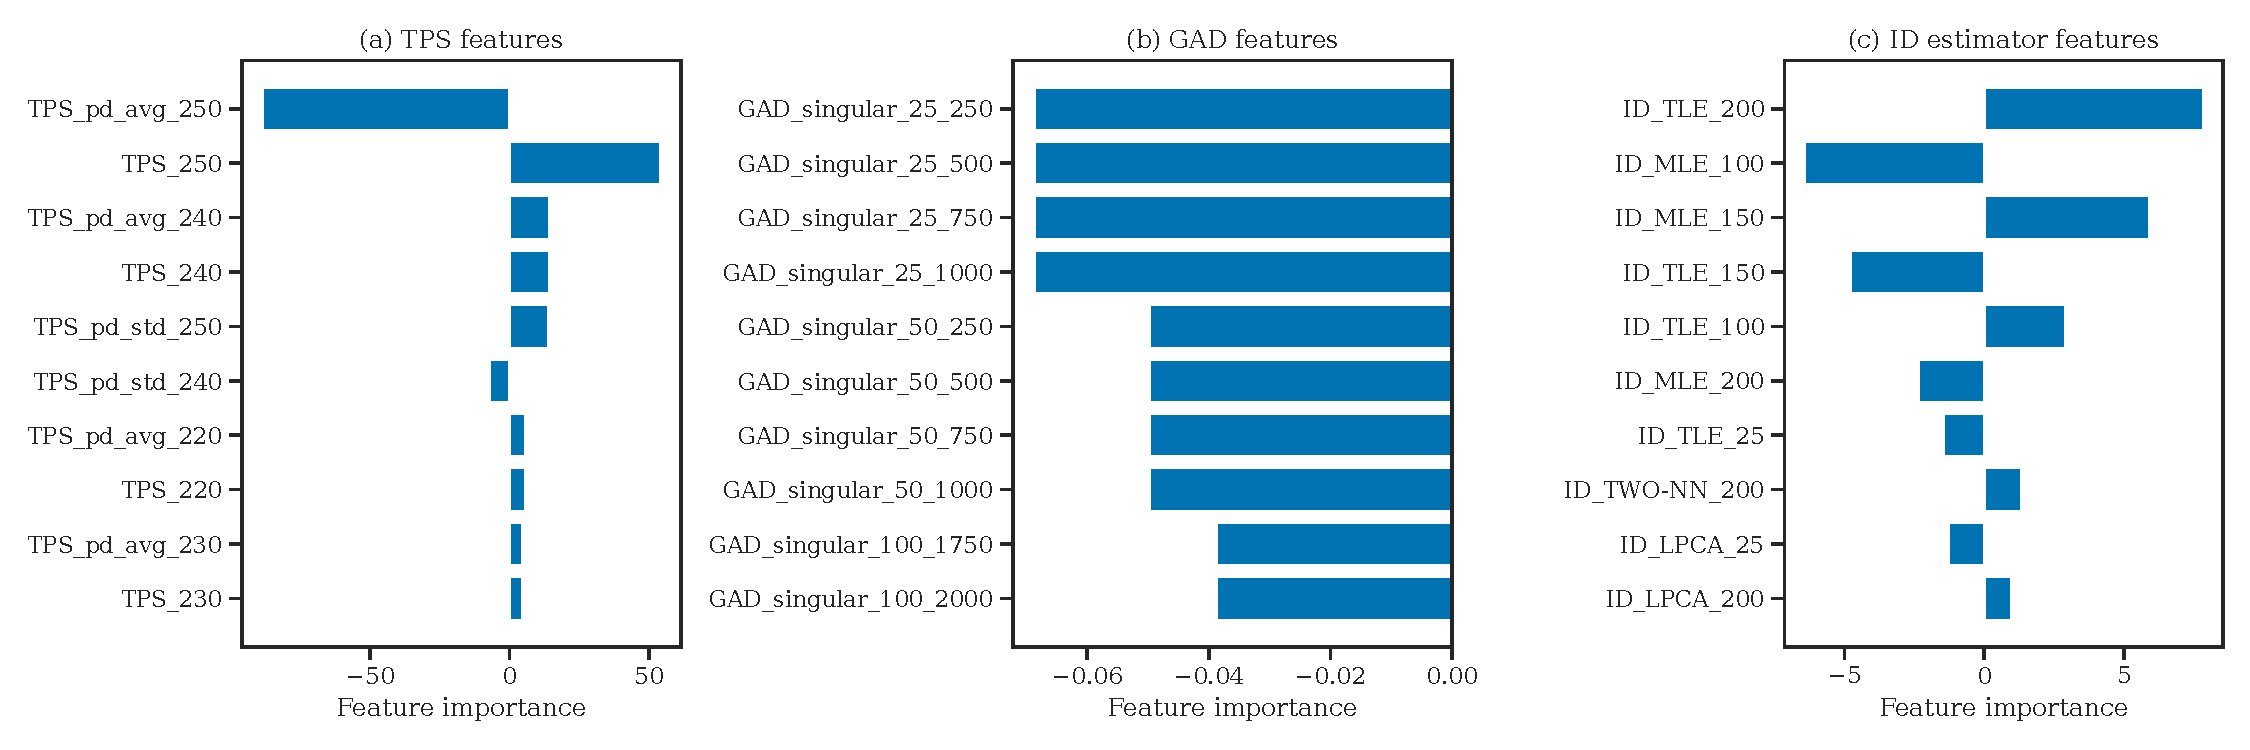
\includegraphics[width=\textwidth]{thesis/figures/bwme-enwiki-top-10-feature-importances-tps-gad-estimated-ids.pdf}
    \caption{Feature importance of the top 10 TPS, GAD and ID estimator features, using the BWME-enwiki model.}
    \label{fig:bwme-enwiki-feature-importances-tps-gad-estimated-ids}
\end{figure}

We have now explained how we trained and evaluated two supervised models for predicting the number of word meanings and whether or not a word is polysemous. Next, we will conclude the thesis and discuss ideas for future work.